%%%%%%%%%%%%%%%%%%%%%%%%%%%%%%%%%%%%%%%%%
% Thesis 
% LaTeX Template
%
%
% Original authors:
% Raphael Wolfisberg 
% 
%
%%%%%%%%%%%%%%%%%%%%%%%%%%%%%%%%%%%%%%%%%

%----------------------------------------------------------------------------------------
%	PREAMBLE: PACKAGES AND OTHER DOCUMENT CONFIGURATIONS
%----------------------------------------------------------------------------------------

\documentclass[11pt, numbers=noenddot, titlepage, a4paper, twoside, onecolumn, DIV=calc]{scrbook} % Paper size, default font size and one-sided paper


\usepackage[ngerman,english]{babel}		%language
\usepackage[T1]{fontenc}
\usepackage[utf8]{inputenc}
\usepackage{lmodern}
% \usepackage{fancyhdr}
\usepackage{setspace}
\usepackage{amsmath} 			%Greek letters
\usepackage{fixltx2e} 			%subscript
\usepackage{multirow}
\usepackage{graphicx}
\usepackage{epstopdf}
\usepackage{pdfpages}
\usepackage{longtable}
\usepackage[outer=23mm]{geometry} %outer margin
\usepackage{textcomp}
\usepackage{tabu}
\usepackage{array}
\usepackage{tabularx}
\usepackage{hyperref,url}
\usepackage[all]{hypcap}
\usepackage{nomencl}
\usepackage{tocloft}
\usepackage{scrpage2}
\usepackage[square, numbers, sort&compress, super]{natbib}
\usepackage{sidecap}
\usepackage{multicol}
\usepackage{float}
\usepackage[bottom, hang]{footmisc}

\usepackage{graphicx} 
\usepackage[hang, bf]{caption}
\setlength{\captionmargin}{20pt}
%\setlength{\abovecaptionskip}{0pt}
%\setlength{\belowcaptionskip}{0pt}
\captionsetup[table]{font=small,skip=0pt}
\captionsetup[figure]{font=scriptsize,skip=0pt}      
\usepackage[font=scriptsize]{caption}


\usepackage{ragged2e}
\usepackage{etoolbox}
\AtBeginEnvironment{multicols}{\RaggedRight}

%\setlength\intextsep{0pt} %space between figures and text..

%\usepackage{float}
%\floatstyle{boxed}
%\restylefloat{figure} if thin borders around all figures are wished

\deftripstyle{raphimen}[0pt][0pt]{\headmark}{}{\pagemark}{}{}{}


\setlength{\skip\footins}{1.5cm}
\setlength{\footnotesep}{0.5cm}
\setlength\footnotemargin{10pt}

\setlength{\cftsecnumwidth}{0pt}
\renewcommand{\cftsecaftersnumb}{\hspace{1.5em}}  % Noident for phantomsections in Contents (Publication Part)

\textheight = 660pt


\graphicspath{{./Pictures/}} % Specifies the directory where pictures are stored


\renewcommand*{\partformat}{\partname~\thepart \thispagestyle{empty}} %remove period after part and remove page number

\setlength\LTleft{0pt}
\setlength\LTright{0pt}


\makenomenclature
%\setlength{\nomitemsep}{1.3pt}
\setlength{\nomitemsep}{-\parsep} %Vertical spacing in Nomenclature

\renewcommand{\nomlabel}[1]{\hspace*{1.5em}#1} %Nomenclature Skip add \dotfill before bracket if dots required...

\let\abk\nomenclature
\setlength{\nomitemsep}{-\parsep}
\makeatletter
\def\thenomenclature{%
  \@ifundefined{chapter}%
  {
    \if@intoc\addcontentsline{toc}{section}{\nomname}\fi%
  }%
  {
    \if@intoc\addcontentsline{toc}{chapter}{\nomname}\fi%
  }%
  \nompreamble
  \list{}{%
    \labelwidth\nom@tempdim
    \leftmargin\labelwidth
    \advance\leftmargin\labelsep
    \itemsep\nomitemsep
    \let\makelabel\nomlabel
  }
}
\makeatother 

\newcommand{\RM}[1]{\MakeUppercase{\romannumeral #1}}


\begin{document}


% Define the page headers using the FancyHdr package and set up for one-sided printing
%\fancyhead{} % Clears all page headers and footers
%\rhead{\thepage} % Sets the right side header to show the page number
%\lhead{} % Clears the left side page header

 % Finally, use the "fancy" page style to implement the FancyHdr headers


\frontmatter % Use roman page numbering style (i, ii, iii, iv...) for the pre-content pages
\pagenumbering{Roman} %Uppercase roman numbering
\setstretch{1.3} % Line spacing of 1.3

\setlength{\footskip}{35mm}



%----------------------------------------------------------------------------------------
%	TITLE PAGE
%----------------------------------------------------------------------------------------


\begin{titlepage}
\begin{flushright}

\includegraphics[scale=0.8, trim= 1mm 1mm 5mm 20mm]{logo} \\[2.9 cm]
\end{flushright}
\begin{center}
{\Huge \bfseries Thesis Title} \\[2 cm]
{\Large Inauguraldissertation \\
der Philosophisch-naturwissenschaftlichen Fakultät \\
der Universität Bern \\[2.2 cm]
{\large vorgelegt von}\\[0.3 cm]
{\LARGE \textsc{Raphael Wolfisberg}} \\[0.3 cm] 
{\large von Neuenkirch, LU} \\ [1.2 cm]
{\Large \emph{Leiter der Arbeit}\\ [0.3 cm]
{\textsc Prof. Dr. Christoph Kempf} \\
and \\
{\textsc Dr. Carlos Ros} \\ [0.9 cm]
Departement für Chemie und Biochemie}}
\end{center}
\end{titlepage}


\clearpage
\setcounter{page}{1}

%----------------------------------------------------------------------------------------
%	DECLARATION
%----------------------------------------------------------------------------------------

\pagestyle{plain}
\phantomsection\addcontentsline{toc}{chapter}{Declaration}
\addtocontents{toc}{\vspace{1em}} % Add a gap in the Contents, for aesthetics
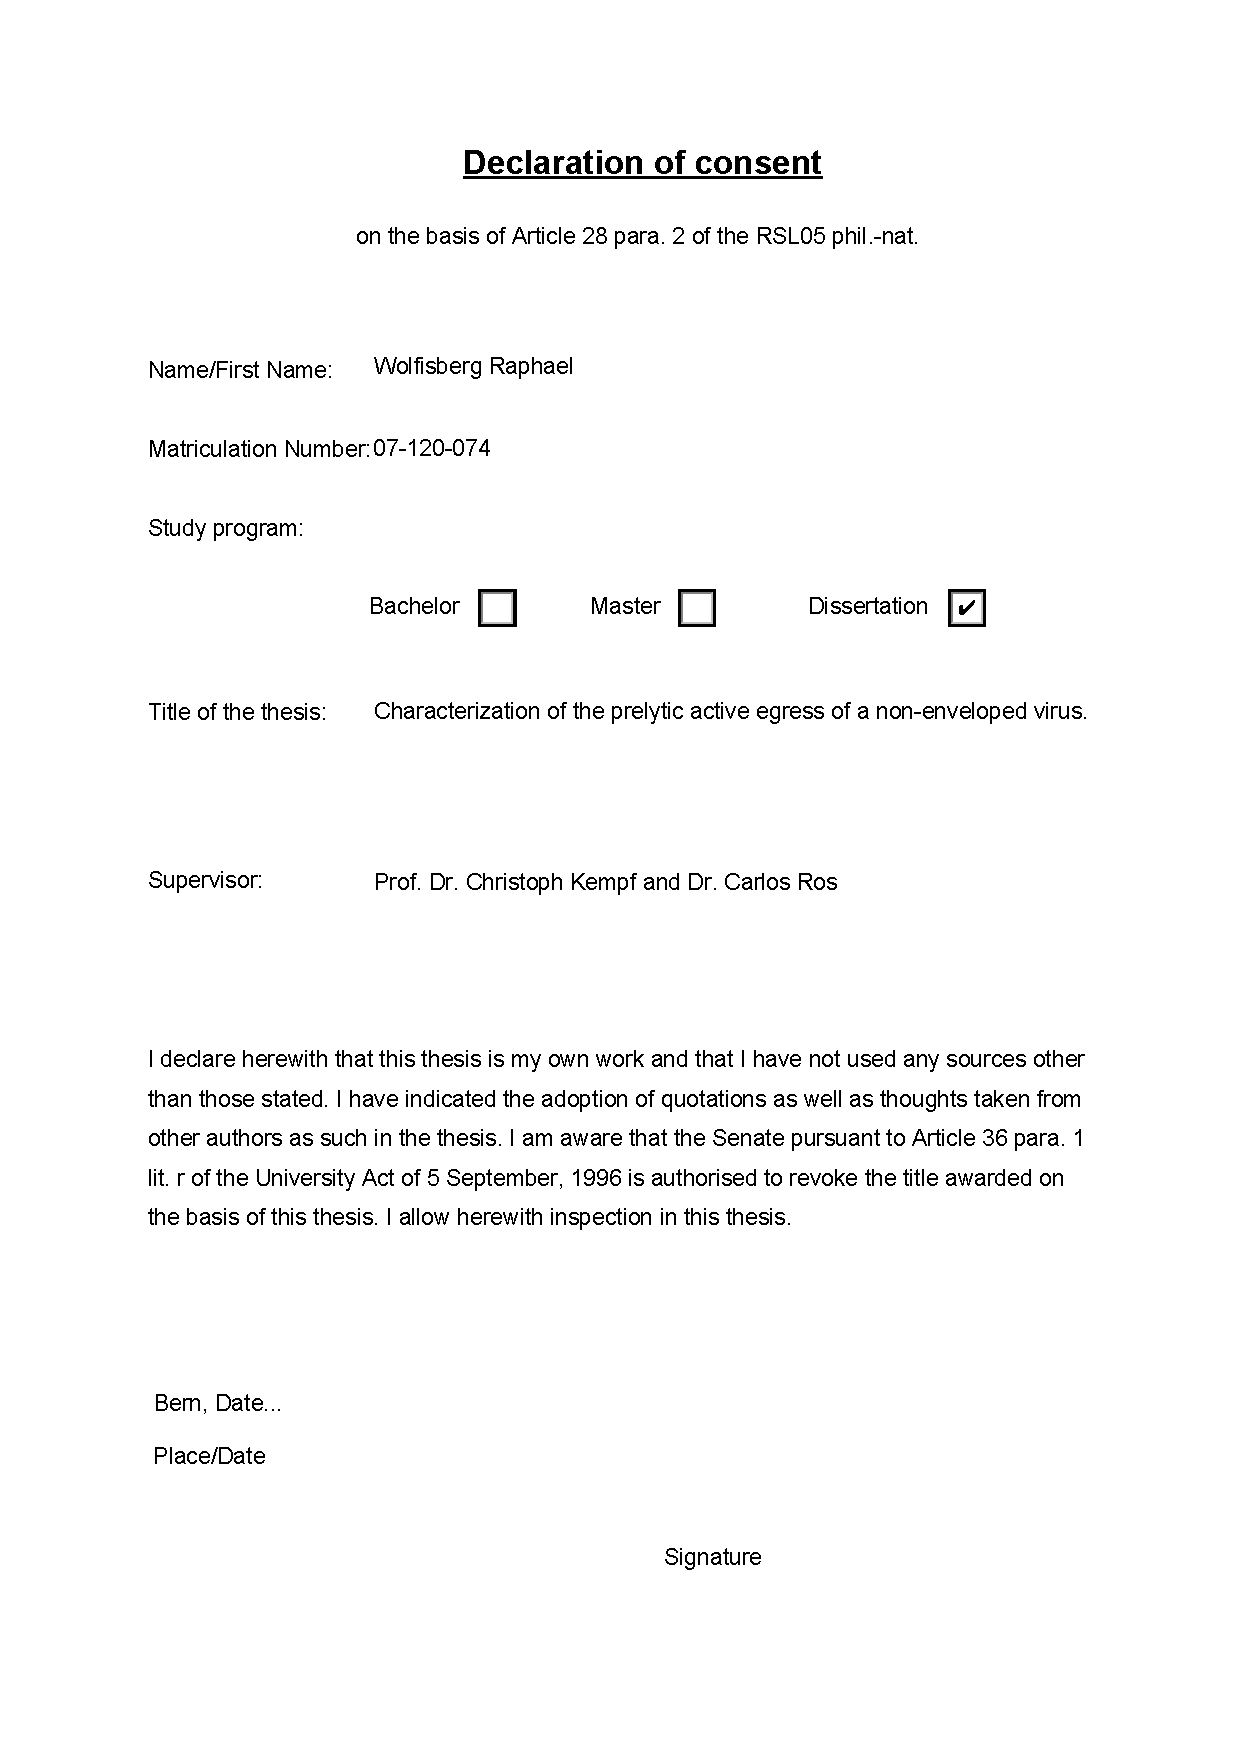
\includepdf[pagecommand=\thispagestyle{plain}]{../pdfdocuments/declaration}

\clearpage







%----------------------------------------------------------------------------------------
%	ABSTRACT PAGE
%----------------------------------------------------------------------------------------
\pagestyle{plain} 

\phantomsection\addcontentsline{toc}{chapter}{Abstract}
\addtocontents{toc}{\vspace{1em}} % Add a gap in the Contents, for aesthetics



The Thesis Abstract is written here (and usually kept to just this page). The page is kept centered vertically so can expand into the blank space above the title too\ldots

\clearpage % Start a new page



%----------------------------------------------------------------------------------------
%	ABBREVIATIONS
%----------------------------------------------------------------------------------------
\pagestyle{plain} % No headers or footers for the following pages


%\setstretch{1.5} % Set the line spacing to 1.5, this makes the following tables easier to read

\phantomsection\addcontentsline{toc}{chapter}{Nomenclature}
\addtocontents{toc}{\vspace{1em}} % Add a gap in the Contents, for aesthetics


\nomenclature{B19V}{Human parvovirus B19}%
\nomenclature{Bp}{Base pair}%


\begin{multicols}{2}[\chapter*{\nomname}] 
 \printnomenclature[1.0 in]
\end{multicols} 







%\l{\emph{Abbreviations}} % Set the left side page header to "Abbreviations"
%\listofsymbols{ll} % Include a list of Abbreviations (a table of two columns)
%{
%\textbf{LAH} & \textbf{L}ist \textbf{A}bbreviations \textbf{H}ere \\
%\textbf{Acronym} & \textbf{W}hat (it) \textbf{S}tands \textbf{F}or \\
%}
\clearpage
%----------------------------------------------------------------------------------------
%	LIST OF CONTENTS/FIGURES/TABLES PAGES
%----------------------------------------------------------------------------------------

\pagestyle{scrheadings} % The page style headers have been "empty" all this time, now use the "fancy" headers as defined before to bring them back



\tableofcontents % Write out the Table of Contents


\listoffigures % Write out the List of Figures


\listoftables % Write out the List of Tables



\clearpage

%----------------------------------------------------------------------------------------
%	THESIS CONTENT - CHAPTERS
%----------------------------------------------------------------------------------------

\mainmatter % Begin numeric (1,2,3...) page numbering


\pagestyle{raphimen}




\part{Introduction}
% Chapter 1

\chapter{Introduction} % Main chapter title

\label{Chapter1} % For referencing the chapter elsewhere, use \ref{Chapter1} 

\lhead{Chapter 1. \emph{Introduction}} % This is for the header on each page - perhaps a shortened title

%----------------------------------------------------------------------------------------
\section{Morphology}

Parvoviruses belong to the smallest of isometric viruses. They are devoid of a lipid envelope and their diameters range from 215 \r{A} (Penaeus stylirostris densovirus, PstDNV) to 255 \r{A} (CPV). The icosahedral nature of parvoviruses was shown unambiguously by X-ray crystallography. The capsid surface of some, particularly invertebrate, parvoviruses appears to be smooth (Galleria mellonella densovirus, GmDNV) whereas others (Adeno-associated virus-2, AAV-2) are spiky at the 3- or 5-fold symmetry axes \cite{pmid10497831, icvt}.      


\nomenclature{PstDNV}{Penaeus stylirostris densovirus}
\nomenclature{GmDNV}{Galleria mellonella densovirus}
\nomenclature{DNA}{Deoxyribonucleic acid}




\section{Physicochemical properties}
about 75 \% protein and 25 \% DNA, Mr about 5.5 - 6.2 x 10\textsuperscript{6}, infectious virion buoyant density is 1.39 - 1.43 gcm\textsuperscript{-3}, in CsCl,mature virions are stable in the presence of lipid solvents, on exposure to pH 3-9 and for most species incubation at 56 \textcelsius~ for 60 min, inactivation occurs by treatment with formalin, $\beta$-propiolacetone, hydroxylamine, ultraviolet light, and oxidizing agentssuch as sodium hypochlorite    

\section{Taxonomy}
The classification of the \textit{Parvoviridae} family is based on morpholological and functional characteristics. Parvoviruses are common animal and insect pathogens that belong to the smallest DNA-containing viruses. Hence the prefix "parvum" which means small in Latin. The name "parvovirus" was first introduced to the literature by Carlos Brailovsky in 1966 \cite{pmid5902774}.   
The \textit{Parvoviridae} family comprises all non-enveloped, isometric, small DNA viruses that contain linear single-stranded genomes. Indeed, parvoviruses are the only viruses in the known biosphere that have both single-stranded and linear DNA genomes. The encapsidated single genomic molecule is 4-6 kb in length and terminates in palindromic duplex hairpin telomers. As a consequence of such a simple genome, parvoviruses are highly dependent on their host for diverse functions in their reproduction \cite{pmid10497831, parvoviruses}. The terminal hairpins are fundamental for the unique replication strategy of the \textit{Parvoviridae} family and hence serve as an invariant hallmark for classification.
Members of the family \textit{Parvoviridae} infect a wide variety of hosts, ranging from insects to primates.
Depending on this feature, the \textit{Parvoviridae} are subdivided into \textit{Parvovirinae} infecting vertebrates and \textit{Densovirinae} infecting insects and other arthropods, respectively. The \textit{Parvovirinae} subfamily is further subdivided into eight genera: \textit{Amdoparvovirus}, \textit{Aveparvovirus}, \textit{Bocaparvovirus}, \textit{Copiparvovirus}, \textit{Dependoparvovirus}, \textit{Erythroparvovirus}, \textit{Protoparvovirus} and \textit{Tetraparvovirus}. The subdivision into the eight genera is based on differences in transcription maps, organization of the ITRs, the ability to replicate efficiently either autonomously or with helper virus and sequence homology amongst the \textit{Parvovirinae} subfamily \cite{pmid11222696, icvt}.

\subsection{The \textit{parvovirinae} subfamily}
   


\subsubsection{\textit{Amdoparvovirus}}
The genus \textit{Amdoparvovirus} shares most characteristics with the genera \textit{Bocaparvovirus} and \textit{Protoarvovirus}. Mature virions exclusively contain negative strand genomic DNA of approximately 4.8 kb in length harbouring dissimilar palindromic sequences at each end \cite{pmid6252342, pmid2843669}. Only two distant species have been reported. Firstly, \textit{Carnivore amdoparvovirus 1}, which comprises only Aleutian mink disease virus (AMDV) and secondly, \textit{Carnivore amdoparvovirus 2}, which encompasses solely gray fox amdovirus (GFAV) \cite{pmid22000359}. 
Permissive replication is tightly restricted to Crandell feline kidney cells. In contrast to the members of the genera \textit{Bocaparvovirus} and \textit{Protoparvovirus}, the virion surface displays three mounds elevated around the threefold icosahedral axis of symmetry. However, several structure features were ascertained to be similar to those found in B19V, CPV, FPV and MVM. Such appearance is comparable to those observed for the genus \textit{Dependoparvovirus} \cite{pmid10400786}. Remarkably, there is no evidence of a phospholipase 2A enzymatic core within the naturally truncated N-VP1 terminus of members belonging to the genus \textit{Amdoparvovirus} as it is common to the other genera of the subfamily \textit{Parvovirinae} \cite{icvt}.       

\nomenclature{AMDV}{Aleutian mink disease virus}
\nomenclature{GFAV}{Gray fox amdovirus}

\subsubsection{\textit{Aveparvovirus}}

\subsubsection{\textit{Copiparvovirus}}

\subsubsection{\textit{Bocaparvovirus}}
The name of the genus is derived from \underline{bo}vine and \underline{ca}nine, referring to the two hosts of the first identified members of this genus.  The genomes of members of the genus \textit{Bocaparvovirus} are quite distinct from all other viruses in the subfamily \textit{Parvovirinae}. As the members of the genera \textit{Protoparvovirus} and \textit{Amdoparvovirus} they contain non-identical imperfect palindromic sequences at both ends of their 5.5 kb genome. Mature virions contain mainly, but not exclusively, negative strand ssDNA \cite{pmid3783814,pmid12441065}.
All RNA transcripts are generated from a single promoter at map unit 4.5. BPV RNA transcripts are alternatively spliced and polyadenylated either at an internal site or at the 3’-end of the genome. Noteworthy, bovine parvovirus (BPV), the main representative, encodes a 22.5 kDa nuclear phosphoprotein, NP-1, whose function still remains unknown. This protein is distinct from any other parvovirus-encoded polypeptide \cite{pmid6319731}.  

\nomenclature{BPV}{Bovine parvovirus}
\nomenclature{kDa}{Kilodalton}
\nomenclature{Da}{Dalton}

\subsubsection{\textit{Dependoparvovirus}}
Positive and negative strand ssDNA is distributed indifferently among mature virions belonging to the genus \textit{Dependoparvovirus} \cite{pmid5014934, pmid5264145}. The 4.7 kb DNA molecule contains identical ITRs of 145 nt, the first 125 nt of which form a palindromic sequence \cite{pmid6246271}. Three mRNA promoters that are located at map units 5, 19 and 40 initiate transcription that can be terminated in two polyadenylation sites located at the right-hand end or alternatively, in the middle of the genome \cite{pmid6253077, pmid6281463}. Common for all currently accepted replication-defective members of the genus \textit{Dependoparvovirus} is their strict dependence upon helper adenoviruses or herpesviruses \cite{pmid4318977, pmid6270377, pmid5227666}. Therefore, their host range tropism strongly depends on the one of the helper virus. 
The only exceptions are the autonomously replicating duck and goose parvoviruses which are also comprised within the \textit{Dependoparvovirus} genus based on phylogenetic analysis \cite{icvt}. The most important members of this genus are the adeno-associated viruses (AAV). They attracted considerable interests since at least one of them, AAV-2, has been reported to integrate site-specifically into human chromosome 19 \cite{pmid2156265, pmid1653762, pmid1334463, pmid1657596}. This characteristic makes AAV a promising candidate for creating viral vectros for gene therapy. As a well characterized member of the \textit{Dependoparvoviruses} AAV-2 represents the model virus among this genus.  


\subsubsection{\textit{Erythroparvovirus}}
Equivalent numbers of positive and negative sense ssDNA are packaged into infectious virions of the genus \textit{Erythroparvovirus}. As in the case with the genus \textit{Dependoparvovirus}, the 5.5 kb ssDNA molecule contains identical ITRs of 383 nt in length at both the 3’ and the 5’ end. The first 365 nt of those secondary elements form palindromic sequences \cite{pmid2408228}. Transcription is regulated by a single mRNA promoter located at map unit 6 \cite{pmid3824910}. A distal polyadenylation site for use in termination of RNA synthesis is located at the far right side. Additionally, transcripts may be terminated at an unusual internal polyadanylation site in the middle of the genome \cite{pmid3599180}. Viruses belonging to this genus are highly erythrotropic, meaning that efficient replication only occurs in rapidly dividing erythroid progenitor cells (EPCs) such as erythroblasts and megakaryocytes present in the bone marrow.
B19V, a human pathogen that causes fifth disease, polyarthropathia, anemic crises in children with underlying hematological diseases (e.g. sickle cell anemia or thalassemia) and intrauterine infections (with hydrops fetalis in some cases) \cite{pmid12097253} represents the model virus among the genus \textit{Erythroparvovirus}. 

\nomenclature{Nt}{Nucleotide}
\nomenclature{ITR}{Inverted terminal repeat}
\nomenclature{Kb}{Kilo base}
\nomenclature{EPC}{Erythroid progenitor cell}


\subsubsection{\textit{Protoparvovirus}}
\textit{Protoparvoviruses} were the first members of the subfamily \textit{Parvovirinae} to be discovered in 1959 \cite{pmid13669314}. Some members of the genus contain positive strand DNA in variable proportions up to 50 \% \cite{pmid6694260}. In mature virions of other members, virtually only negative strand DNA occurs. What they have in common are their hairpin structures at both the 5’ and 3’ ends of the linear 5 kb ssDNA molecule that differ in both sequence and predicted structure \cite{pmid6298737}. Transcription of the genome is regulated by two mRNA promoters at map units 4 and 39 \cite{pmid6828378}. There is only one polyadenylation site at the 3’ end. 
Viral replication provokes characteristic cytopathic effects in cell culture. Many species display hemagglutination with erythrocytes of one or several species. The genus \textit{Protoparvovirus} is primarily represented by MVM \cite{icvt, parvoviruses}.       

\subsubsection{\textit{Tetraparvovirus}}





\begin{longtable}{@{\extracolsep{\fill}}l l l l l}

\setlength\LTleft{0pt}
\setlength\LTright{0pt}

\textbf{Genus} & \textbf{Species} & \textbf{Virus or virus variants} & \textbf{Abbreviation} & \textbf{Accession \#}\\
\hline
\textit{Amdoparvovirus} & \textbf{\textit{Carnivore amdoparvovirus 1}} & Aleutian mink disease virus & AMDV & JN040434 \\
 & \textit{Carnivore amdoparvovirus 2} & Gray fox amdovirus & GFAV & JN202450 \\
\textit{Aveparvovirus} & \textit{\textbf{Galliform aveparvovirus 1}} & Chicken parvovirus & ChPV & GU214704 \\
& & Turkey parvovirus & TuPV & GU214706 \\
\textit{Bocaparvovirus} & \textit{Carnivore bocaparvovirus 1} & Canine minute virus & CnMV & FJ214110 \\
& \textit{Carnivore bocaparvovirus 2} & Canine bocavirus 1 & CBoV & JN648103 \\
& \textit{Carnivore bocaparvovirus 3} & Feline bocavirus & FBoV & JQ692585 \\
& \textit{Pinniped bocaparvovirus 1} & California sea lion bocavirus 1 & CslBoV1 & JN420361\\
& & California sea lion bocavirus 2 & CslBoV2 & JN420366 \\
& \textit{Pinniped bocaparvovirus 2} & California sea lion bocavirus 3 & CslBoV3 & JN420365 \\
 & \textit{Primate bocaparvovirus 1} & Human bocavirus 1 & HBoV1 & JQ923422 \\
 & & Human bocavirus 3 & HBoV3 & EU918736 \\
 & & Gorilla bocavirus & GBoV & HM145750 \\
 & \textit{Primate bocaparvovirus 2} & Human bocavirus 2a & HBoV2a & FJ973558 \\
 & & Human bocavirus 2b & HBoV2b & FJ973560 \\
 & & Human bocavirus 2c & HBoV2c & FJ170278 \\
 & & Human bocavirus 4 & HBoV4 & FJ973561 \\
 & \textit{\textbf{Ungulate bocaparvovirus 1}} & Bovine parvovirus & BPV & DQ335247 \\
 & \textit{Ungulate bocaparvovirus 2} & Porcine bocavirus 1 & PBoV1 & HM053693 \\ 
 & & Porcine bocavirus 2 & PBoV2 & HM053694 \\
 & & Porcine bocavirus 6 & PBoV6 & HQ291309 \\
 & \textit{Ungulate bocaparvovirus 3} & Porcine bocavirus 5 & PBoV5 & HQ223038 \\
 & \textit{Ungulate bocaparvovirus 4} & Porcine bocavirus 7 & PBoV7 & HQ291308 \\ 
 & \textit{Ungulate bocaparvovirus 5} & Porcine bocavirus 3 & PBoV3 & JF429834 \\ 
 & & Porcine bocavirus 4-1 & PBoV4-1 & JF429835 \\
 & & Porcine bocavirus 4-2 & PBoV4-2 & JF429836 \\
 \textit{Copiparvovirus} & \textit{\textbf{Ungulate copiparvovirus 1}} & Bovine parvovirus 2 & BPV2 & AF406966 \\
 & \textit{Ungulate copiparvovirus 2} & Porcine parvovirus 4 & PPV4 & GQ387499 \\
 \textit{Dependoparvovirus} & \textit{\textbf{Adeno-associated dependoparvovirus A}} & Adeno-associated virus-1 & AAV1 & AF063497 \\ 
 & & Adeno-associated virus-2 & AAV2 & AF043303 \\
 & & Adeno-associated virus-3 & AAV3 & AF028705 \\
 & & Adeno-associated virus-4 & AAV4 & U89790 \\
 & & Adeno-associated virus-6 & AAV6 & AF028704 \\
 & & Adeno-associated virus-7 & AAV7 & AF513851 \\
 & & Adeno-associated virus-8 & AAV8 & AF513852 \\
 & & Adeno-associated virus-9 & AAV9 & AX753250 \\
 & & Adeno-associated virus-10 & AAV10 & AY631965 \\ 
 & & Adeno-associated virus-11 & AAV11 & AY631966 \\ 
 & & Adeno-associated virus-12 & AAV12 & DQ813647 \\
 & & Adeno-associated virus-13 & AAV13 & EU285562 \\
 & & Adeno-associated virus-S17 & AAVS17 & AY695376 \\
 & \textit{Adeno-associated dependovirus B} & Adeno-associated virus-5 & AAV5 & AF085716 \\
 & & Bovine adeno-associated virus & BAAV & AY388617 \\
 & & Caprine adeno-associated virus & CapAAV & DQ335246 \\
 & \textit{Anseriform dependoparvovirus 1} & Duck parvovirus & DPV & U22967 \\
 & & Goose parvovirus-PT & GPV2 & JF926695 \\
 & & Goose parvovirus & GPV & U25749 \\
 & \textit{Avian dependovirus 1} & Avian adeno-associated virus & AAAV & AY186198 \\
 & \textit{Chiropteran dependoparvovirus 1} & Bat adeno-associated virus & BtAAV & GU226971 \\
 & \textit{Pinniped dependoparvovirus 1} & California sea lion adeno-associated virus & CslAAV & JN420372 \\
 & \textit{Squamate dependoparvovirus 1} & Snake adeno-associated virus & SAAV & AY349010 \\
 \textit{Erythroparvovirus} & \textit{\textbf{Primate erythroparvovirus 1}} & Human parvovirus B19-Au & B19V-Au & M13178 \\
 & & Human parvovirus B19-J35 & B19V-J35 & AY386330 \\
 & & Human parvovirus B19-Wi & B19V-Wi & M24682 \\
 & & Human parvovirus B19-A6 & B19V-A6 & AY064475 \\
 & & Human parvovirus B19-Lali & B19V-Lali & AY044266 \\
 & & Human parvovirus B19-V9 & B19V-V9 & AJ249437 \\
 & & Human parvovirus B19-D91 & B19V-D91 & AY083234 \\
 & \textit{Primate erythroparvovirus 2} & Simian parvovirus & SPV & U26342 \\
 & \textit{Primate erythroparvovirus 3} & Rhesus macaque parvovirus & RhMPV & AF221122 \\
 & \textit{Primate erythroparvovirus 4} & Pig-tailed macaque parvovirus & PtMPV & AF221123 \\
 & \textit{Rodent erythroparvovirus 1} & Chipmunk parvovirus & ChpPV & GQ200736 \\
 & \textit{Ungulate erythroparvovirus 1} & Bovine parvovirus 3 & BPV3 & AF406967 \\
 \textit{Protoparvovirus} & \textit{Carnivore protoparvovirus 1} & Feline parvovirus & FPV & EU659111 \\ 
 & & Canine parvovirus & CPV & M19296 \\
 & & Mink enteritis virus & MEV & D00765 \\
 & & Racoon parvovirus & RaPV & JN867610 \\
 & \textit{Primate protoparvovirus 1} & Bufavirus 1a & BuPV1a & JX027296 \\
 & & Bufavirus 1b & BuPV1b & JX027295 \\
 & & Bufavirus 2 & BuPV2 & JX027297 \\
 & \textit{\textbf{Rodent protoparvovirus 1}} & H-1 parvovirus & H1 & X01457 \\
 & & Kilham rat virus & KRV & AF321230 \\
 & & LuIII virus & LuIII & M81888 \\
 & & Minute virus of mice (prototype) & MVMp & J02275 \\
 & & Minute virus of mice (immunosuppressive) & MVMi & M12032 \\
 & & Minute virus of mice (Missouri) & MVMm & DQ196317 \\
 & & Minute virus of mice (Cutter) & MVMc & U34256 \\
 & & Mouse parvovirus 1 & MPV1 & U12469 \\
 & & Mouse parvovirus 2 & MPV2 & DQ196319 \\
 & & Mouse parvovirus 3 & MPV3 & DQ199631 \\
 & & Mouse parvovirus 4 & MPV4 & FJ440683 \\
 & & Mouse parvovirus 5 & MPV5 & FJ441297 \\
 & & Hamster parvovirus & HaPV & U34255 \\ 
 & & Tumor virus X & TVX & In preparation \\
 & & Rat minute virus 1 & RMV1 & AF332882 \\
 & \textit{Rodent protoparvovirus 2} & Rat parvovirus 1 & RPV1 & AF036710 \\
 & \textit{Ungulate protoparvovirus 1} & Porcine parvovirus Kresse & PPV-Kr & U44978 \\
 & & Porcine parvovirus NADL-2 & PPV-NADL2 & L23427 \\
 \textit{Tetraparvovirus} & \textit{Chiropteran tetraparvovirus 1} & Eidolon Helvum (bat) parvovirus & Ba-PARV4 & JQ037753 \\
 & \textit{\textbf{Primate tetraparvovirus 1}} Human parvovirus 4 G1 & PARV4G1 & AY622943 \\
 & & Human parv4 G2 & PARV4G2 & DQ873391 \\      
 & & Human parv4 G3 & PARV4G3 & EU874248 \\
 & & Chipmanzee parv4 & Ch-PARV4 & HQ113143 \\
 & \textit{Ungulate tetraparvovirus 1} & Bovine hokovirus 1 & B-PARV4-1 & EU200669 \\
 & & Bovine hokovirus 2 & B-PARV4-2 & JF504697 \\
 & \textit{Ungulate tetraparvovirus 2} & Porcine hokovirus & P-PARV4 & EU200677 \\
 & \textit{Ungulate tetraparvovirus 3} & Porcine Cn virus & CnP-PARV4 & GU938300 \\
 & \textit{Ungulate tetraparvovirus 4} & Ovine hokovirus & O-PARV4 & JF504699 \\
     




\end{longtable}





\section{Tropism}
Most parvoviruses, such as MVM, \nomenclature{MVM}{Minute virus of mice} CPV \nomenclature{CPV}{Canine parvovirus} and FPV, \nomenclature{FPV}{Feline parvovirus} show specific host ranges and tissue tropisms. The majority of the parvoviruses are members of those tightly controlled viruses. However, some parvoviruses, as for example many of the AAVs, \nomenclature{AAV}{Adeno-associated virus} infect many hosts and a variety of tissues. Understanding controls of these properties for autonomous parvoviruses show great promise for the therapeutic delivery to be controlled or modified in gene therapy applications \cite{pmid12941411}.  

To date, two independent strains of the parvovirus MVM have been described to occur in mice. Both strains display disparate \textit{in vitro} tropism and \textit{in vivo} pathogenicity despite differing by only 14 amino acids in their capsid proteins. Fist, MVMp, \nomenclature{MVMp}{Prototype strain of MVM} the prototype strain, was originally isolated from a contaminated murine adenovirus stock and was shown to replicate efficiently in mouse fibroblasts \cite{pmid5945715}. Secondly, MVMi,\nomenclature{MVMi}{Immunosuppressive strain of MVM} the immunosuppressive strain, was recovered from an infected EL-4 T-cell lymphoma culture \cite{ pmid1244418}. Although MVMi infection may result in pathology of infected mice, it has been shown that the infection more likely interferes with numerous T-cell functions \textit{in vitro}. The infection rather causes problems for the ongoing study the mice are being used for as the immune system will be activated, the activity of T-lymphocytes or B-lymphocytes will be altered and tumor formation may be suppressed \cite{pmid6457871, pmid6264106, pmid11528091}.

	As above-mentioned, it has been shown that the allotropic MVM strains, MVMi and MVMp, differ in their target cell tropism. In order to map the viral sequences responsible for that difference, chimeric viral genomes were constructed \textit{in vitro} from infectious genomic clones of both strains. The differences in the cell tropism between MVMi and MVMp have been mapped to the capsid gene, in particular to the VP2 residues 317 and 321. Both residues are located at the base of the threefold spike of the virion and are involved in controlling the cell tropism of the two distinct MVM strains \cite{pmid3357208, pmid3392768, pmid3257270}.  Interestingly, residue 321 aligns with residue 323 of CPV, that itself is a critical determinant for CPV host range tropism. Further residues (VP2 residues 399, 553 and 558) were identified in MVMi to be able to confer fibrotropism to single site-directed mutants. Those residues cluster around the twofold dimple-like depression \cite{pmid9817841}. 
	
	In general, tissue tropism determining amino acids were found be located on, or near, the viral surface, mainly by raised structural elements around the threefold axes of symmetry. Differences in tropism and pathogenicity have also been mapped to the capsid proteins of Aleutian mink disease parvovirus \cite{pmid8396664}, porcine parvovirus (PPV) \nomenclature{PPV}{Porcine parvovirus} \cite{pmid8642680}, CPV \cite{pmid3176341, pmid1331498}, and FPV \cite{pmid7513918} in a capsid region analogous to that observed for MVM. Although the same structural element of viruses is involved in mediating host and tissue tropisms, each appears to be affecting a different mechanism. Host ranges of CPV and FPV are controlled by receptor binding, whereas the cell tropisms of MVM appear to be due to restrictions of interactions with intracellular factors \cite{pmid9817841, pmid12941411}.


%----------------------------------------------------------------------------------------

\section{Structure}

\subsection{Parvoviruses in general}

Parvovirus capsids are devoid of a lipid envelope and have an average diameter of 18 to 26 nm. The viral capsid is made up of 60 copies of between two and four structural proteins that overlap each other. For each virus there is one major capsid protein present in the capsid structure. Minor proteins form the same core structure, but differ in the sequence length on their amino termini. The capsid proteins display a T=1 icosahedral symmetry and are variously designated VP1-VP4. Thus, the capsid has a 5-3-2 point group symmetry containing 31 rotational symmetry elements that intersect at the center: six fivefolds, ten threefolds, and fifteen twofolds. 
Despite the differences in protein forms and the low homology between some of the viruses, several structural elements on the capsid surface are common to most parvoviruses. These include raised cylindrical channels at the fivefold axes surrounded by depressed, canyon-like regions. Further shared surface characteristics are protrusions at the threefold axes, termed as spikes or peaks, and dimple-like depressions at the icosahedral twofold axes.  
A common feature of parvoviruses is their high resistance to physicochemical treatments. This stability provides an effective protection to the fragile, condensed genome in the extracellular environment ensuring transmission between their hosts. The ssDNA \nomenclature{ssDNA}{Single stranded DNA } genome consists of approximately 5000 bases, packed as either a positive or, more usually, as a negative sense strand. At the 5’ and 3’ ends, the genome harbors palindromic sequences of about 120 to 250 nucleotides, that form secondary hairpin structures which are essential for the initiation of viral genome replication \cite{pmid16242744, pmid25555192, pmid8392729, pmid9817841, pmid11827486, pmid2006420, pmid12941411}. \\      

\nomenclature{dsDNA}{Double stranded DNA}








\subsection{MVM}

Both DNA-containing full and empty particles were crystallized in the monoclinic space group C2. Following data processing and refinement, the resulting electron density map was interpreted with respect to the amino acid sequence of MVMi. The known CPV structure was used as a phasing model since 52 \% of the 578 amino acids in VP2 of MVM are identical to CPV. The polypeptide chain of the major structural protein, VP2, could be traced from residue 39 to residue 587 at the C-terminus \cite{pmid15299974}.     
The common c-terminal part of the structural proteins has an eight-stranded antiparallel $\beta$-barrel topology, frequently found in viral capsid proteins \cite{pmid2673017}. Large loops between the $\beta$-strands of the $\beta$-barrel that form the principal surface features, particularly the threefold spikes, and determine host-range tropism were found to be quite dissimilar in MVM and CPV. 
The first 37 amino acids are not visible in the electron density map. Since the N-VP2 terminal part contains a predominantly poly-glycine conserved sequence, it might be highly flexible. There is density extending along the fivefold channels of the MVMi capsid that was modeled as the glycine-rich N-terminal region \cite{pmid15299494, pmid8969301}. \textit{In vitro}, trypsin digestion of full MVM virions results in a truncated VP3 polypeptide that still contains the glycine-rich sequence. In this way, most VP2 N-termini can be cleaved. These findings suggest that there is a dynamic situation at the fivefold channel. In one model, one in five amino termini are externalized along the fivefold axes and are accessible for cleavage. Newly created, cleaved N-VP3 termini could withdraw into the virion and be replaced at the surface by an uncleaved N-VP2 terminus. \cite{pmid8503170, pmid9817841}.
A substantial amount of internal electron density could be related to 10 DNA nucleotides that were previously found in the analysis of the structure of CPV \cite{pmid7735832, pmid1616694}. For MVM, 19 additional DNA nucleotides were identified in a difference electron-density map with respect to the data of empty particles. Thus, 29 ordered, or partially ordered, nucleotides per icosahedral asymmetric unit imply that approximately 34 \% of the total genome display icosahedral symmetry. This finding, and the conservation of base-binding sites between MVMi and CPV, identifies a DNA-recognition site on the parvoviral capsid interior \cite{pmid9817841}.    










\section{Nucleic Acid}

\subsection{Genome organization}


\subsection{Transcriptome}

\section{Viral proteins}

\subsection{Structural Proteins}

\subsection{Non-structural proteins}
 

%----------------------------------------------------------------------------------------

\section{}


\subsection{}



\subsection{}


% Chapter 2

\chapter{Methods} % Main chapter title

\label{Chapter2} % For referencing the chapter elsewhere, use \ref{Chapter2} 

\lhead{Chapter 2. \emph{Methods}} % This is for the header on each page - perhaps a shortened title

%----------------------------------------------------------------------------------------

\section{Cell Cultures}
A9 ouab\textsuperscript{r}l1 cells, a derivative from the original HGPRT\textsuperscript{-} L-cell line A9 represent a clone resistant to 10\textsuperscript{-3} M ouabain after nitrosoguanidine mutagenesis \cite{pmid14213660}.
NB324K cells are a clone of SV40-transformed \nomenclature{SV40}{Simian vacuolating virus 40 or Simian virus 40} human newborn kidney cells \cite{pmid13911591}. The SV40 large T antigen was detected by immunofluorescent \nomenclature{IF}{Immunofluorescence} staining with monoclonal antibodies \cite{pmid6169844}. \nomenclature{mAb}{Monoclonal antibody} However, NB324K cells do not produce infectious SV40 spontaneously.
Both cell lines, A9 mouse fibroblasts and NB324K cells, were routinely propagated under a minimal number of passages in DMEM \nomenclature{DMEM}{Dulbecco modified Eagle's medium}supplemented with 5 \% of heat inactivated fetal bovine serum at 37 \textcelsius~ in 5 \% CO\textsubscript{2} atmosphere. \nomenclature{FCS}{Fetal calf serum} 


\subsection{Freezing and thawing of cells}
Before use the A9 mouse fibroblasts or NB324K cells were thawed at 37 \textcelsius~ and cultured in 5 mL of pre-warmed DMEM supplemented with 5 \% FCS. The medium was replaced every 3 to 4 days. 
In order to freeze the cells for long storage in liquid nitrogen they were passed the day before, to ensure exponential growth. Subsequently, 7.5 \% DMSO was added and the cells were frozen slowly at -70 \textcelsius~ over night before transfer to liquid nitrogen.

%----------------------------------------------------------------------------------------

\section{Virus Stocks}
\label{Virus Stocks}
Stocks of MVM without detectable levels of VP3 were propagated on A9 mouse fibroblast monolayers. As soon as the cytopathic effect became evident, the supernatant \nomenclature{SN}{Supernatant}was collected and pre-cleared from cell debris by low-speed centrifugation. Thereby, intracellular, VP3 rich capsids were discarded. In order to remove low-molecular contaminants, virus containing SN was pelleted through 20 \% sucrose cushion in PBS by ultra-centrifugation. Virus titers were determined by qPCR \nomenclature{qPCR}{Quantitative PCR} \nomenclature{PCR}{Polymerase chain reaction} as DNA-packaged particles per microliter.   

\subsection{Separation of empty and full capsids}

Sucrose purified capsids were prepared as previously described in section \ref{Virus Stocks}, page \pageref{Virus Stocks}. The virus pellet was resuspended in 10 mL PBS. Caesium chloride was added to a density of 1.38 g/mL adjusted by refractometry ($\eta$=1.371) at 4 \textcelsius. The gradient was centrifuged to equilibrium for 24 h at 41000 rpm and 4 \textcelsius~ in a Beckmann SW-41 Ti rotor. Gradients were fractionated and tested for intact capsids by dot blot analysis using B7 mAb. CsCl was depleted from the corresponding fractions by size-exclusion chromatography through PD-10 desalting columns and concentrated by ultra-centrifugation when required.          
   
   








\section{Freezing bacteria stocks in glycerol}
Bacteria were frozen in dry ice. A volume of 700 $\mu$L of the bacteria culture that was grown over night in LB-medium was mixed with 300 $\mu$L of 50 \% glycerol in a cryotube. In order to mix well the glycerol the cryotube was vortexed intensively. Following snap-freeze in dry ice the bacteria were stored at -70 \textcelsius.



\section{Anion-exchange chromatography}
A Mono Q HR 5/5 (Pharmacia) column (5 x 50 mm) was used to analyse viral samples. The Mono Q column was connected to the ÄKTAmicro chromatography system (GE Healthcare) that was operated by the UNICORN control software. The Mono Q column was equilibrated with six column volumes (CV) starting buffer (20 mM Tris-HCl, 1 mM EDTA, pH 7.2). Samples (1 mL) containing at least 10\textsuperscript{10} virus particles in 10 mM Tris-HCl, 1 mM EDTA, pH 8 were applied to the Mono Q column trough a 2 mL loop. After eluting the protein, which did not bind to the column in the starting buffer, a linear salt gradient (0-2 M NaCl) in 20 mM Trsi-HCl, 1 mM EDTA, pH 7.2, was applied. Fractions of 0.185 mL were collected in 96-well plates. Viral genomes in each fraction were quantified by qPCR. All buffers were filtered and degassed before application to the Mono Q column. 





\section{Quantitative PCR}
Amplification of MVM DNA and real-time detection of PCR products were performed by using BioRad CFX96 technology with SYBR green supermix. PCR was carried out by using the hot-start iTaq\textsuperscript{\texttrademark} DNA polymerase (Bio-Rad Laboratories) following the manufacturer’s guide-lines. Viral DNA was isolated using DNeasy blood and tissue kit. Elution of the purified vDNA was carried out using 100 $\mu$L elution buffer. As templates 2 $\mu$L of the isolated viral DNA were used for the PCR reaction and were added to the following master mix:\\

\begin{table}[h]
\begin{center}
\begin{tabular}{l r r}
\textbf{Component} & \textbf{Amount} & \textbf{Final concentration}\\
\hline
dH\textsubscript{2}O, PCR grade & 6 $\mu$L & -\\
Forward primer, 10 pM & 1 $\mu$L & 0.5 pM\\
Reverse primer, 10 pM & 1 $\mu$L & 0.5 pM\\
2x IQ\textsuperscript{\texttrademark} SYBR\textsuperscript{\textregistered} Green Supermix & 10 $\mu$L & 1x\\
\hline
\textbf{Total volume} & \textbf{18 $\boldsymbol{\mu}$L} & \\
\end{tabular}
\end{center}
\label{Master mix}
\caption[Master mix for quantitative PCR]{Master mix for quantitative PCR. In order to minimize pipetting errors a master mix was prepared. Following preparation the master mix was distributed across the 96 well plates. The master mix contains all the ingredients which are required for the DNA amplification except the initial DNA template that differs among the samples.}
\end{table} 

To ensure accurate quantification, the 96-well plates containing master mix and template DNA were shortly spun and transferred into the BioRad CFX96 unit. The following PCR program was used for quantification of viral DNA:

\begin{table}[h]
\begin{center}
\begin{tabular}{r l r r}
\textbf{Cycles} & \textbf{Step} & \textbf{Temperature} & \textbf{Time}\\
\hline
1x & Initial denaturation & 95 \textcelsius & 300 s\\
40x & Denaturation & 95 \textcelsius & 15 s \\
 & Annealing & 61 \textcelsius & 15 s \\
 & Extension & 72 \textcelsius & 15 s \\
1x & Final denaturation & 95 \textcelsius & 60 s \\
1x & Melting curve & 65 \textcelsius~up to 95 \textcelsius & 0.1 \textcelsius/s \\
\end{tabular} 
\end{center} 
\label{PCR conditions}
\caption[PCR conditions]
   {PCR conditions for the amplification and real-time detection of MVM DNA.}
\end{table}

To provide standards for sample quantification, serially diluted plasmids containing the entire MVM genomic DNA were used.
For cell number variations that may exist between the samples, the number of applied cells per PCR reaction needed to be quantified for normalization as well. For this purpose quantification of cellular $\beta$-actin gene was performed. After normalization, direct comparison of the results is possible. $\beta$-actin quantification was carried out with the same PCR conditions outlined in table \ref{PCR conditions}, \pageref{PCR conditions}.



\subsection{Immunoprecipitation}
Either \textit{in vitro} treated viruses or viruses from cell extracts were transferred to LoBind tubes that were pre-blocked with PBS containing 1 \% bovine serum albumin (PBSA 1 \%). The volume was adjusted to 200 $\mu$L with PBSA 1 \%. The antibody was added in excess and incubated with the viral capsids for 1 h at 4 \textcelsius~ on a rotary shaker. Subsequently, 20 $\mu$L protein G-agarose beads were added. Following overnight incubation at 4 \textcelsius~ and centrifugation at 2500 rpm for 5 min the supernatant was discarded. The beads were washed 4 times with PBSA 1 \%. To remove the BSA an additional wash step was carried out with PBS. Finally, the beads were frozen at -20 \textcelsius~ until further use or immediately processed. 

\nomenclature{IP}{Immunoprecipitation}

\subsection{}
 

%----------------------------------------------------------------------------------------

\section{}


\subsection{}



\subsection{}

 
% Chapter 3

\chapter{Morphology} % Main chapter title

\label{Chapter3} % For referencing the chapter elsewhere, use \ref{Chapter2} 


%----------------------------------------------------------------------------------------

\label{sec:Morphology}

Parvoviruses belong to the smallest of isometric viruses. A linear single-stranded DNA genome of about 5 kb is packaged into the virus capsid \cite{pmid4975639, pmid5264145, pmid5429749}. They are non-enveloped and their diameters range from 215 \r{A} (Penaeus stylirostris densovirus, PstDNV) to 255 \r{A} (CPV) \cite{pmid10497831, icvt}. 

The icosahedral nature of parvoviruses was shown unambiguously by a combination of electron microscopy (EM) and, latterly, X-ray crystallography \cite{pmid2006420}. Interpretation of the structural data gave rise to three distinct types of surface topology among parvoviruses (see Figure~\ref{Morphology}, p.~\pageref{Morphology}) \cite{pmid15795290}. The icosahedral twofold axes and the protrusions surrounding the icosahedral threefold axes display profound surface topology differences between each group. Types I and III comprise members of the \textit{Parvovirinae} subfamily described in Section~\ref{sec: The Parvovirinae subfamily}, see p.~\pageref{sec: The Parvovirinae subfamily}. They share in common the following surface features: a protrusion at the 3-fold axis, depressed regions between the 3-fold elevated regions at the 2-fold axis, and another depressed region encerceling the 5-fold axis. These two groups mainly differ in the shape of the 3-fold elevated region. 

Members of the genus \textit{Protoparvovirus}, as for example CPV, FPV, MVM, and PPV, represent the first topology group that is characterized by a single, relatively flat, pinwheel-shaped protrusion at the icosahedral threefold axes and a wider twofold dimple. The third topology group encompasses the AMDV, B19V, AAV2, AAV4, and AAV5 capsids, which show three distinct mounds at a distance of $\sim$20-26 \r{A} from the icosahedral threefold axes. In addition, the depression at the twofold axis appears to be slightly deeper, particularly for B19V \cite{pmid20375175, pmid12136130, tropism}. In contrast to the vertebrate parvoviruses, no large surface protrusions or depressions are present in \textit{Densovirus} capsids that appeared to be relatively spherical and featureless, adopting a second topology group \cite{pmid15769470, pmid9817847}.        


\begin{figure}[h] 
\centering
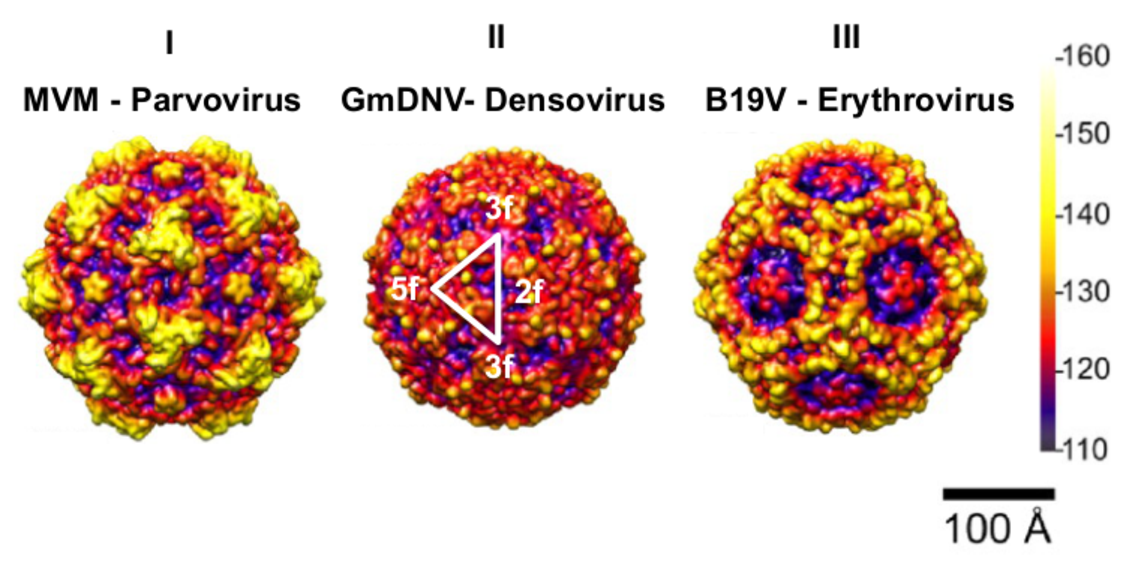
\includegraphics[width=0.9\textwidth]{Morphology}
\caption[Parvovirus surface topology groups]{Surface topology groups among members of the \textit{Parvoviridae} family. Stereo, depth cued (blue-red-yellow-white), and space-filling capsid surface illustration of representative members of the two subfamilies of the parvoviruses. Type viruses representing the three surface topology groups (I-III) and the genus to which they belong are indicated. A viral asymmetric unit bound (white triangle) is shown by a 2-fold (2f), two 3-folds (3f) and a 5-fold (5f) axis on the GmDNV image. A horizontal scale bar (100 \r{A}) for diameter measurement and a vertical color bar depicting color cueing as a function of particle radius in \r{A} are shown on the right hand side. These images were computed from atomic coordinates using the UCSF-Chimera program \cite{pmid15264254}, and all are rendered at the same resolution (7.9 \r{A}) and magnification. The figure was adapted from \cite{pmid20375175}.}
\label{Morphology}
\end{figure}

%The capsid surface of some, particularly invertebrate, parvoviruses appears to be smooth (Galleria mellonella densovirus, GmDNV) whereas others (Adeno-associated virus-2, AAV-2) are spiky at the 3- or 5-fold symmetry axes \cite{pmid10497831, icvt}.      


\nomenclature{PstDNV}{Penaeus stylirostris densovirus}
\nomenclature{GmDNV}{Galleria mellonella densovirus}
\nomenclature{DNA}{Deoxyribonucleic acid}

% Chapter 4

\chapter{The rugged virion} % Main chapter title

\label{Chapter4} % For referencing the chapter elsewhere, use \ref{Chapter2} 


%----------------------------------------------------------------------------------------


\section{Physicochemical Properties}
\label{Physicoprop}
The extracellular infectious virus entity is defined as virion. An infectious parvovirus virion only consists of two components, namely of about 75~\% protein and 25~\% DNA. Their molecular weight (MW) is approximately 5.5-6.2~$\times$~10\textsuperscript{6} dalton. The virion buoyant density is 1.39 to 1.43 gcm\textsuperscript{-3}, measured in CsCl gradients \cite{CsCl, pmid4317344}. Since parvoviruses are devoid of a lipid envelope, mature virions are stable in the presence of lipid solvents. In particular, animal parvoviruses show considerable heat resistance. Most species resist alcohol or ether treatment, exposure to pH 3-10, or incubation at 60 \textcelsius~ for 60 min \cite{pmid12935806, pmid12385412, pmid17880601, pmid19039515, pmid14660623, pmid10941577, pmid10662625}, hence they are clearly more stable compared to most other, especially enveloped, viruses. Only harsh conditions, such as treatment with formalin, $\beta$-propiolacetone, hydroxylamine, ultraviolet light, and oxidizing agents as for example sodium hypochlorite, ensure effective virus inactivation \cite{pmid4213983, pmid3416941, pmid7848502, pmid1520981}. Accordingly, the capsid effectively protects the fragile, condensed genome from detrimental biological, chemical, and physical agents, thus ensuring efficient transmission of the virion through the extracellular environment.     

\section{Atomic Model}
\label{Structure}
Currently, there is no crystal structure available for MVMp DNA containing particles. Only baculovirus-expressed MVMp-like particles and empty capsids (ECs) have been determined at a resolution of 3.25 \r{A} and 3.75 \r{A}, respectively \cite{pmid16103145}. For MVMi both DNA-containing full and empty particles were crystallized and determined at 3.5 \r{A} resolution. The known CPV structure \cite{pmid3379641} was used as a phasing model with 52~\% of the 587 amino acids in VP2 of MVMi being identical to CPV. Following molecular replacement and refinement, the resulting electron density map was interpreted with respect to the amino acid sequence of MVMi. The polypeptide chain of the major structural protein, VP2, could be traced from residue 39 to residue 587 at the C-terminus (see Figure~\ref{Structure1}, p.~\pageref{Structure1}) \cite{pmid15299974}. The N-terminal extensions of VP1 and VP2 are not visible in the electron density map. The capsid displays a T=1 icosahedral symmetry, thus having a 5-3-2 point group symmetry containing 31 rotational symmetry axes that intersect at the center: six fivefolds, ten threefolds, and fifteen twofolds. The C-terminal part in common of the structural proteins has an eight-stranded ($\beta$B to $\beta$I) antiparallel $\beta$-barrel topology, referred to as jellyroll motif (reviewed in \cite{pmid2673017, Fundamental_Virology}). This structural motif is frequently found in other virus capsid proteins. Additionally, like many other viruses, parvoviruses have a ninth $\beta$A-strand which is hydrogen-bonded to the $\beta$B-strand. The high structural conservation of the jellyroll motif among parvoviruses is remarkable considering the low sequence homology between members of this family. Large loops between the $\beta$-strands of the $\beta$-barrel that form the principal surface features, particularly the threefold spikes, confer the surface biological properties of the capsid, such as determination of host tropism \cite{pmid1316457, pmid3942033} and sites of antigenicity \cite{pmid8985402, pmid1942246}. Such loops were found to be quite dissimilar in different parvoviruses (see Figure~\ref{Structure1}, p.~\pageref{Structure1}) \cite{pmid8503170}. 

The lack of the first 38 amino acids of VP2 indicates a highly disordered structure for N-VP2 \cite{pmid15299974}. Indeed, a glycine-rich conserved sequence at the N-terminal part of VP2 contributes to its flexibility. In virions, but not in ECs, additional density seen within the fivefold channels was modeled and found to represent the predominantly poly-glycine conserved sequence \cite{pmid15299494, pmid8969301}. These findings suggest that the N-terminus of VP2 is highly dynamic as DNA packaging triggers externalization of one in five N-termini along the pores of the fivefold axis \cite{pmid9817841}.
 
A substantial amount of electron density in the capsid interior was built as 10 DNA nts which were located at equivalent positions to those previously found in the analysis of the structure of CPV \cite{pmid7735832, pmid1616694}. For MVM, 19 additional nts were identified in a difference electron-density map with respect to the data of empty particles. Altogether, these 29 ordered, or partially ordered, nts per icosahedral asymmetric unit imply that approximately 34~\% of the total viral genome display icosahedral symmetry. These findings, and the conservation between the base-binding sites of MVMi and CPV, has led to the identification of a DNA-recognition site on the parvoviral capsid interior \cite{pmid9817841}.    

\begin{figure}
\centering
  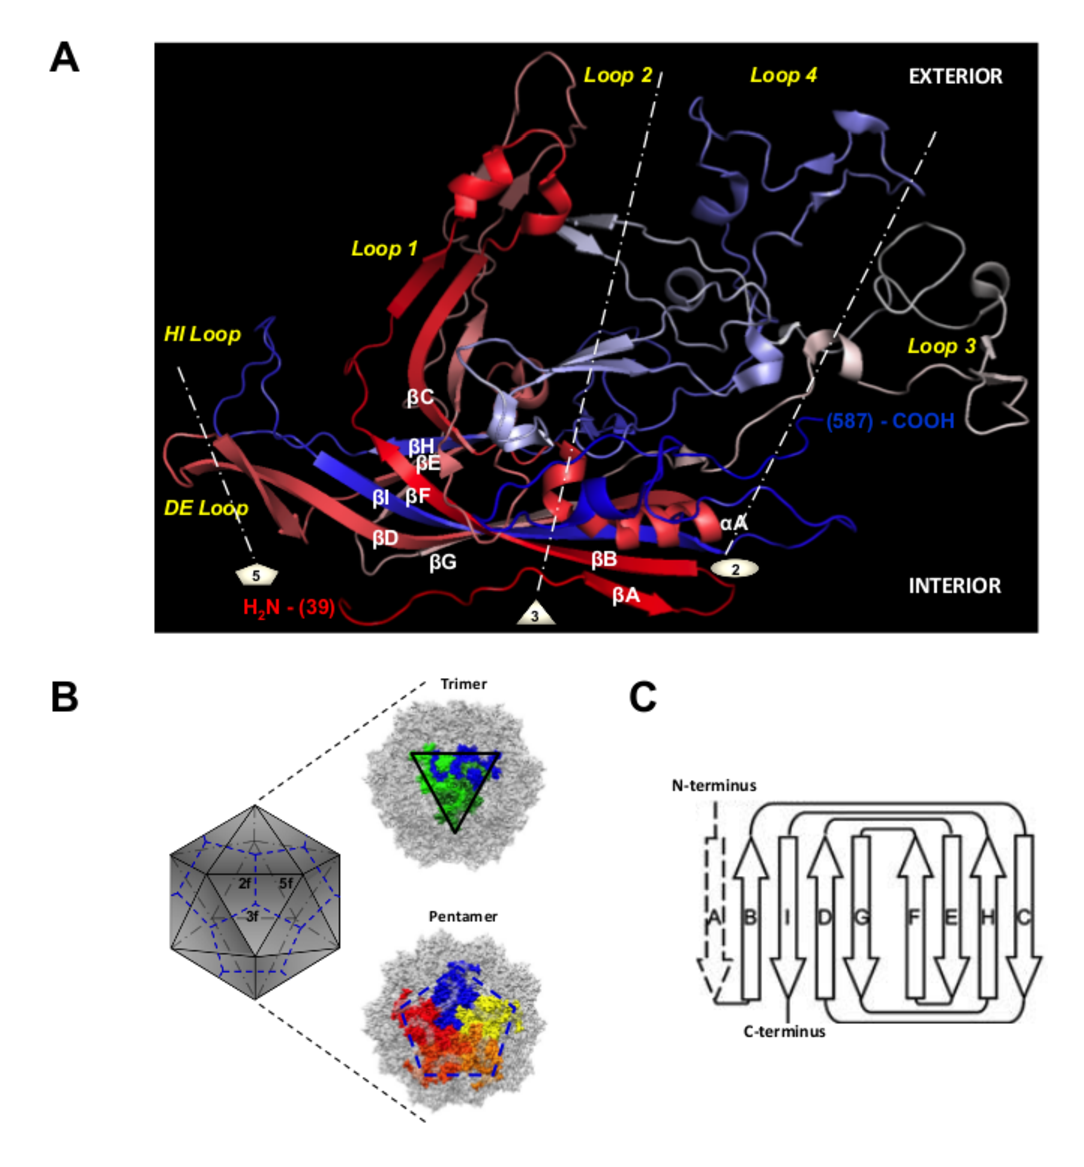
\includegraphics[scale=0.55]{Structure}
  \caption[Structure of MVM]
   {Atomic model of MVM. \textbf{(A)} Ribbon diagram of MVMp VP2 illustrating $\beta$-strands, helical and loop regions. The amino acid sequence is gradually colored in a red–white–blue spectrum, beginning at residue 39 and ending at the C-terminal residue 587. The highly conserved $\alpha$A-helix $\beta$-barrel motif, consisting of two antiparallel $\beta$-sheets ($\beta$ABIDG–$\beta$FEHC), are labeled. The icosahedral twofold (oval), threefold (triangle), and fivefold (pentagon) axes are indicated. Atomic coordinates for MVMp were obtained from RSCB protein database (PDB accession number 1Z14). The illustration was generated using the PyMol program \cite{PyMol}. \textbf{(B)} 60 copies of the capsid proteins form a T=1 icosahedral structure. Each triangle of the icosadeltahedron designates a virus capsid protein subunit. Rotational symmetry axes are referred to as 5f, 3f and 2f, representing 5-folds, 3-folds, and 2-folds, respectively. A VP trimer (assembly intermediate) and a VP pentamer are represented on the right hand side, superimposed on the capsid surface. The representation was generated using the UCSF-Chimera program \cite{pmid15264254} by computing the same atomic coordinates as mentioned in (A). \textbf{(C)} The connectivity of the antiparallel $\beta$ strands (arrows) of the jellyroll $\beta$-barrel is schematically indicated. Strand A is dashed because it is conserved among parvoviruses and a number of other viruses but it is not present in all viruses. This illustration was adapted from \cite{Structure}} 
\label{Structure1}
\end{figure}

%\textit{In vitro}, trypsin digestion of full MVM virions results in a truncated VP3 polypeptide that still contains the glycine-rich sequence. In this way, most VP2 N-termini can be cleaved. These findings suggest that there is a dynamic situation at the fivefold channel. In one model, one in five amino termini are externalized along the fivefold axes and are accessible for cleavage. Newly created, cleaved N-VP3 termini could withdraw into the virion and be replaced at the surface by an uncleaved N-VP2 terminus. \cite{pmid8503170, pmid9817841}.

\section{Structural Proteins}
\label{VPs}

The MVM capsid is made up of 60 copies of a single polypeptide sequence. The virion contains structural proteins of three size classes (VP1-VP3) that constitute a nested set. These share the same C-terminal core structure, but differ in the sequence length on their N-termini. The capsid is assembled from about 10 copies per particle of VP1 (83 kDa), whereas VP2 (64 kDa) represents the major species \cite{pmid988192}. In DNA containing virions, the N-terminal region of VP2 is cleaved during cell entry by intracellular proteolytic digestion to generate VP3 (60 kDa), which displays a truncation of approximately 25 amino acids at its N-terminus (see Section~\ref{Rearrangements}, p.~\pageref{Rearrangements}) \cite{pmid864702, pmid1448928, pmid982825, pmid9770425}. The N-terminal cleavage of VP2 does not occur in ECs, suggesting that DNA packaging into the particle allows the N-VP2 terminus to be externalized \cite{pmid3296697, pmid6481856, pmid864702}. The processing of VP2 in full virions can be mimicked \textit{in vitro} by digestion with tryptic proteases, as for instance chymotrypsin or trypsin. However, the proteolytic site \textit{in vivo} is different to the chymotrypsin- or trypsin-sensitive site \cite{pmid6481856, pmid864702, pmid1448928}. Although containing the identical amino acid sequence that is cleaved in VP2, VP1 does not appear to be cleaved at this position in either type of particle, \textit{in vivo} or \textit{in vitro}. VP2 is both necessary and sufficient for the assembly and encapsidation of viral ssDNA (see Sections~\ref{Assembly} and~\ref{Packaging}, p.~\pageref{Assembly}~-~\pageref{Packaging}) \cite{pmid10662625}. However, VP1 is required to produce an infectious particle since capsids that lack VP1 were blocked subsequent to cell binding and prior to the initiation of DNA replication, thus they are unable to fulfill a complete viral life cycle \cite{pmid8416366}. Indeed, the 142 amino acid N-terminal extension of VP1 which is referred to as VP1 unique region (VP1u) harbors several important motifs to initiate viral infection. Two of which are a PLA\textsubscript{2} motif as well as a nuclear localization signal (NLS), elaborated in Section~\ref{Motif}, p.~\pageref{Motif}. Since VP1u initially is sequestered within the viral shell, the incoming virion must undergo important structural changes \textit{in vivo} in order to expose its functional domains on the capsid surface. By treatment of purified virions under controlled temperature or with urea, VP1u exposure could be demonstrated \textit{in vitro} \cite{pmid9927584, pmid15194745}. 
    
\section{Functional Domains}
\label{Motif}

From the atomic model of parvoviruses it can be estimated that structural proteins of 25-30 kDa theoretically suffice to constitute a capsid to protect the viral genome. However, this minimum size is generally enlarged among parvoviruses. VP1 and VP2 exceed the minimum size more than twice as much. The additional parts of the structural proteins harbor essential functional motifs that mediate a number of processes in the infectious viral life cycle. These include host cell surface receptor recognition (see Section~\ref{Binding}, p.~\pageref{Binding}), entry and escape from endosomes (see Sections~\ref{Endocytosis} to~\ref{Escape}, pp.~\pageref{Endocytosis} -~\pageref{Escape}), nuclear localization (see Section~\ref{Localization}, p.~\pageref{Localization}), DNA packaging, nuclear export, tropism and pathogenicity determinants (see Chapter~\ref{Chapter5}, p.~\pageref{Chapter5}), immune surveillance and final maturation of particles to produce infectious virus progeny \cite{PLA2}.    

\subsection{The Phospholipase A\textsubscript{2} (PLA\textsubscript{2}) Motif}
\label{PLA2}

In the VP1u region of all parvoviruses, except AMDV and the members of the genus \textit{Brevidensovirus}, as well as \textit{Tetraparvovirus}, a PLA\textsubscript{2} motif has been identified \cite{pmid11702787}. The calcium binding loop (YXGXG) and the catalytic histidine-aspartic acid dyad (HDXXY) of parvoviral phospholipases are related to Ca\textsuperscript{2+}-dependent extracellular or secretory sPLA\textsubscript{2}s which are found for example in bee and snake venoms. Unlike all previously characterized sPLA\textsubscript{2}s, the viral sPLA\textsubscript{2} motifs show very weak sequence similarity and lack the characteristic multiple disulfide bonds, thus analogy is mainly restricted to the catalytic units. PLA\textsubscript{2}s specifically catalyze the hydrolysis of phospholipid substrates at the 2-acyl ester (\textit{sn}-2) position to release free fatty acids and lysophospholipids. The viral sPLA\textsubscript{2}s hydrolyze all major classes of glycerophospholipids, except phosphatidylinositol, without displaying a preference for unsaturated \textit{versus} saturated \textit{sn}-2 fatty acyl chains \cite{pmid14726513}. The catalytic activity of the PLA\textsubscript{2} is dependent on Ca\textsuperscript{2+} in mM concentrations and reaches a maximum at a pH range 6-7, presumably associated with the deprotonation of the His residue in the catalytic dyad at such pH \cite{pmid9115999, pmid7574497}.

The biological importance of the viral PLA\textsubscript{2} motif was demonstrated by mutational analyses with AAV2, MVM, and PPV \cite{pmid16284249, pmid11702787, pmid20974479}. Viruses lacking a functional PLA\textsubscript{2} motif were not infectious as they failed to escape from endosomes \cite{pmid16284249, pmid14644609,  pmid11799199, pmid11961250}.               

\begin{figure}
\centering
  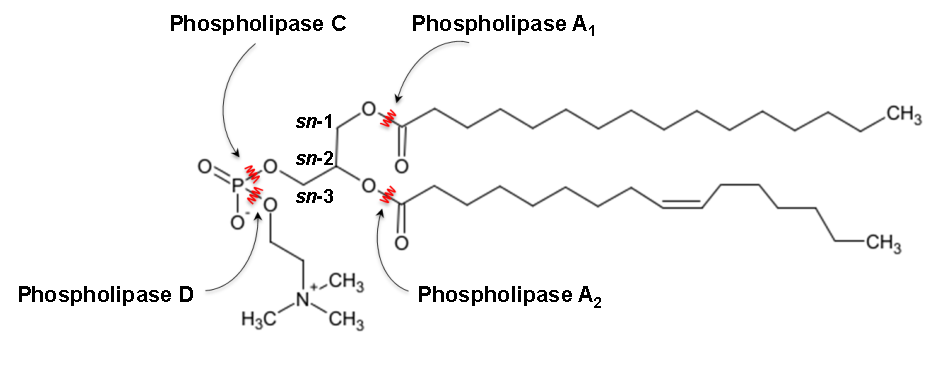
\includegraphics[scale=0.7]{PLA}
  \caption[The cleavage sites of different types of PLAs]
   {The cleavage sites of the different PLAs are illustrated using phosphatidylcholine (PC), a common phospholipid, as an example. Phospholipase A\textsubscript{1}, A\textsubscript{2}, C, and D specifically cleave different ester bonds in the phospholipid. Their respective sites of attack are represented by red staggered lines.} 
\label{PLA}
\end{figure}

\subsection{The Nuclear Localization Signal (NLS)}
\label{NLS1}
In addition to the PLA\textsubscript{2} motif \cite{pmid11702787}, the VP1u region of MVM contains four basic clusters (BCs) of amino acids, referred to as BC1 to BC4. These are highly conserved among parvoviruses and moreover, even in some other DNA viruses. BC1 and BC2 represent conventional NLS which are characterized by a short stretch of basic amino acids \cite{pmid6096007, pmid6088992}. BC3 and BC4, which are separated by a short spacing sequence in between, may rather be arranged as a bipartite NLS domain \cite{pmid1991323}. The clustered basic amino acids interact with transport receptors of the importin/karyopherin family which mediate nuclear import \cite{pmid9126736, pmid9759490, pmid12067655}. Nuclear transport activity has been demonstrated for BC1 in the context of a singly expressed VP1 protein \cite{pmid12072505} and as NLS-peptide coupled to an heterologous carrier protein \cite{pmid9428689}. Furthermore, it is proven to be essential for CPV infectivity \cite{pmid11799183} and for MVM to initiate infection \cite{pmid12072505}. In contrast, BC3 and BC4 did not show such capacity to import VP1 either expressed alone \cite{pmid9428689} or in the context of the complete MVM genome \cite{pmid12072505}. Alternatively, these BCs may be involved in the tethering of the ssDNA genome to the capsid inner surface. Such function has been demonstrated for two basic, significantly homologous DNA-binding domains of the protein J of the $\phi$X174 bacteriophage \cite{pmid11991963}.

\begin{figure}
\centering
  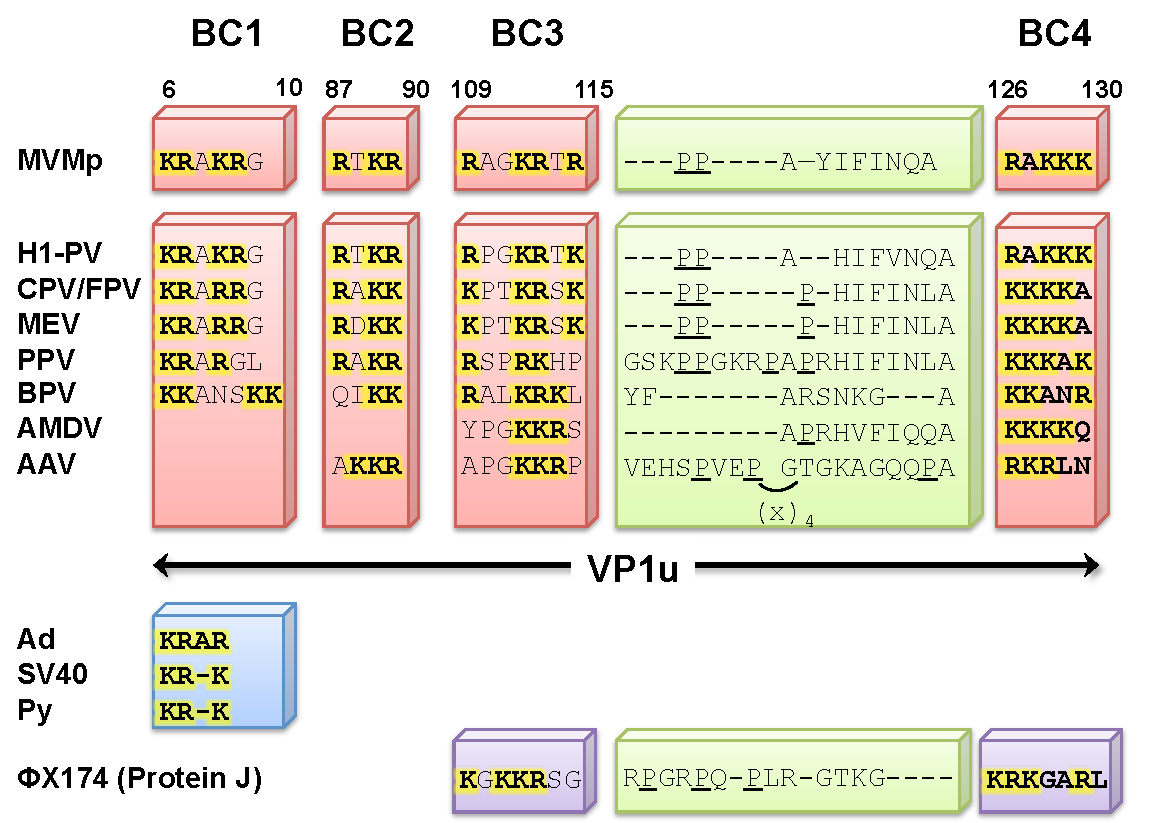
\includegraphics[scale=0.6]{NLS}
  \caption[Nuclear localisation signal (NLS)]
   {VP1 nuclear targeting sequences. The alignment of BCs (BC1 to BC4), which are conserved in the VP1u region among parvoviruses, is boxed in red. Amino acid residues are abbreviated using the single letter code. Sequence homology between BC1 and other karyophilic double-stranded DNA (dsDNA) viruses is shaded in blue on the left-hand side. Conservation of BC3 and BC4 with the protein J of the ssDNA bacteriophage $\phi$X174 is boxed in magenta on the right-hand side. Basic residues of the BC boxes are represented in bold face and possible homologous residues in the spacing region (boxed in green) between BC3 and BC4 are shadowed. Characteristic proline residues which are scattered along the space region are underlined. This illustration was adapted from \cite{pmid12072505, almendral}.}
\label{NLS}
\end{figure}


\subsection{The Nuclear Localization Motif (NLM)}
\label{NLM1}
Since both VP1 and VP2 singly expressed proteins efficiently target the nucleus of transfected cells \cite{pmid8416366, pmid12072505} each protein must carry its own nuclear transport sequence. The common C-terminal sequence of VP1 and VP2 lacks a conventional consensus NLS. However, VP2 contains one single region which is enriched in basic amino acids (528-KGKLTMRAKLR-538) near its C-terminus. Based on the crystal structure \cite{pmid9817841, pmid2006420}, analysis revealed that this sequence is structurally ordered as a $\beta$-sheet which forms the carboxy half of the $\beta$I strand (residues 520 to 538) of the eight-stranded antiparallel $\beta$-barrel (see Figure~\ref{NLM}, p.~\pageref{NLM}). Moreover, the $\beta$I-strand shows marked amphiphatic characteristics, exposing all the basic amino acids to the solvent in the interior surface of the capsid while the hydrophobic residues face toward the protein core. Mutational analysis revealed that the basic nature of the exposed face of $\beta$I, as well as the hydrophobic residues on the opposite face, conferred a nuclear localization capacity to the VP2 protein. Accordingly, this sequence in $\beta$I which only functions under a precise conformation, but not in a linear form, is referred to as the VP2 nuclear localization motif (NLM) \cite{pmid10729155}.        

\begin{figure}
\centering
  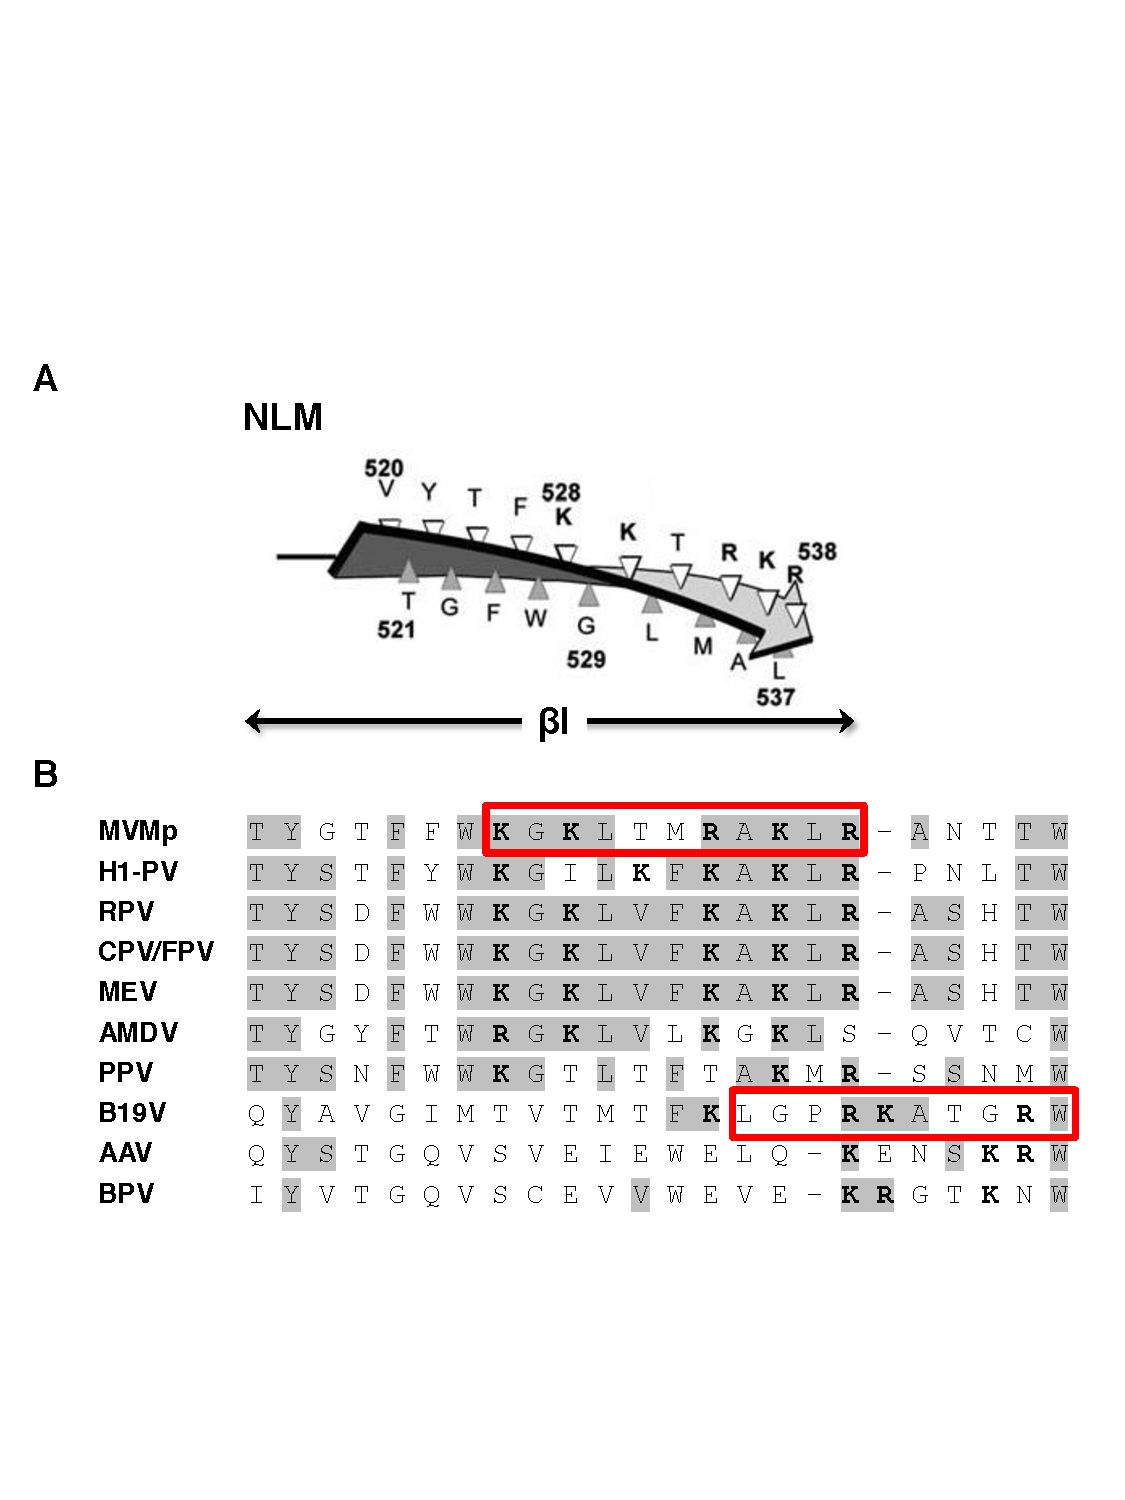
\includegraphics[scale=0.7]{NLM}
  \caption[Nuclear localisation motif (NLM)]
   {Nuclear localization motif (NLM). \textbf{(A)} Schematic representation of the VP2 NLM of MVM as disposed on the $\beta$-strand I of the antiparallel, eight-stranded $\beta$-barrel topology in the common C-terminal part of VP1 and VP2. Basic amino acids which are exposed to the solvent are represented in bold. \textbf{(B)} Alignment of the NLM that is conserved among parvoviruses. Homologous positions are shadowed and basic residues are in bold. Sequences with proven nuclear localization capacity are boxed in red. This illustration was adapted from \cite{pmid10729155, almendral}.} 
\label{NLM}
\end{figure}


\nomenclature{NLS}{Nuclear localization signal}
\nomenclature{NLM}{Nuclear localization motif}
\nomenclature{dsDNA}{Double-stranded DNA}
\nomenclature{ssDNA}{Single-stranded DNA}
\nomenclature{sPLA\textsubscript{2}}{Secretory PLA\textsubscript{2}}
\nomenclature{NPC}{Nuclear pore complex}
\nomenclature{BC}{Basic cluster}
\nomenclature{H1-PV}{Parvovirus H1}
\nomenclature{MW}{Molecular weight}
 
% Chapter 5

\chapter{Genome Architecture} % Main chapter title

\label{Chapter5} % For referencing the chapter elsewhere, use \ref{Chapter2} 

% \lhead{Chapter 2. \emph{Methods}} % This is for the header on each page - perhaps a shortened title

%----------------------------------------------------------------------------------------



\label{sec: Architecture}
The MVM genome is a small, non-permutated, linear, single-stranded DNA molecule \cite{pmid789912, pmid225040, Genome1, Genome2} that is \np{5085} nt in length for MVMi and \np{5149} nt for MVMp \cite{pmid3502703}. The relatively long coding sequence of approximately 4.8 kb contains two major, monosense ORFs that span most of the viral genome, with some regions having overlapping coding regions \cite{pmid6298737}. The ORFs encode a non-structural (NS) gene and a structural (VP) gene, by convention termed as occupying the "left" or the "right" half of the coding sequence, respectively. The NS gene encodes four proteins that are required for the replication of the viral genome and are referred to as NS1, NS2\textsuperscript{P}, NS2\textsuperscript{Y}, and NS2\textsuperscript{L}. The VP gene encodes an overlapping set of capsid proteins, VP1 the minor capsid protein and VP2 the major capsid protein \cite{pmid6828378, pmid2939261, pmid2942705}. A representation of the genomic organization of MVM is illustrated in Figure~\ref{Architecture}~A, p.~\pageref{Architecture}.   

\section{The MVM Left- and Right-End Telomeres}        

The coding sequence is bracketed by short, imperfect palindromes which form back on themselves to secondary structured duplex telomeres. Both telomeres differ considerably from each other in size, primary sequence and secondary structure \cite{pmid6298737}. Hence, they are physically and functionally disparate and vary in their terminal resolution strategies at the two sites (see Section~\ref{Resolution}, p.~\pageref{Resolution}), although the molecular principles that underlie both strategies are very similar \cite{encapsidation}. 

Firstly, the MVM left-end telomere is 121 nt in length and forms into a Y-shaped configuration. Its structure is depicted in Figure~\ref{Architecture}~B (left panel), p.~\pageref{Architecture}. The stem region which contains 43 base pairs (bp) only is interrupted by a mismatched bubble sequence where a triplet GAA on the inboard arm is opposed to the dinucleotide sequence GA on the outboard arm. Additionally, an asymmetric thymidine residue is located within the stem on the outboard arm in the immediate proximity to the "ears" that are generated by small internal palindromes. These "ear"-like structures give rise to the Y-shaped configuration of the left-end terminus \cite{pmid225040, pmid6298737, pmid3973977, replication}. A single DNA sequence, designated the "flip" sequence, is conserved in the progeny viral left-end telomere, as is observed \textit{in vivo} \cite{pmid3973977}.  

Secondly, the MVM right-end telomere is 248 nt in length and is most simply depicted as an almost perfect duplex stem structure of 121 bp. The palindrome only is interrupted by a triplet of unpaired nts that forms a small asymmetric bubble near the distal end of one strand, along with three unpaired bases which form the cross-link at the palindrome axis \cite{pmid6298737, pmid3973977}. As in homotelomeric parvoviruses, two distinct forms of the MVM right-end terminus, referred to as "flip" and "flop", are generated in equimolar amounts \textit{in vivo} (see Figure~\ref{Architecture}~D (i) and (ii), p.~\pageref{Architecture}) \cite{telomere2, encapsidation}. These two forms are the inverted complements of one another and both give rise to viral origins, dubbed \textit{oriR} \cite{pmid1388310, pmid9765384, pmid10627544}. A small internal palindrome, surrounding the three-nt bubble, thermodynamically enables an alternative, asymmetric cruciform configuration of the right-end telomere (see Figure~\ref{Architecture}~D (iii), p.~\pageref{Architecture}) \cite{pmid6602687}. 


\subsection{Terminal Resolution \textit{versus} Asymmetric Junction Resolution}
\label{Resolution}

As is the case for most of the heterotelomeric parvoviruses, MVM shows packaging bias with minus strands preferentially encapsidated to plus strands by a 10-100-fold margin (see Section~\ref{Packaging}, p.~\pageref{Packaging}) \cite{pmid6828378, pmid3296697}. This results from differences in the efficiency of their two DNA replication origins at both ends of their genomes, rather than any strand-specific packaging sequence. In particular, the efficient nick site of the \textit{oriR} dictates the negative polarity of the packaged strand which is encapsidated in MVM virions \cite{pmid15681430}. 

Given the fact that alike their homotelomeric cousins, the right-end hairpin of MVM exists as an equimolar mix of flip and flop sequence orientations, it is processed by a similar terminal resolution strategy. Nicking of the hairpin near the junction between palindromic and non-palindromic sequences and subsequent extension of the right-end terminus allows an efficient inversion of the palindrome (see step iii and iv in Figure~\ref{RHR}, p.~\pageref{RHR}). On the contrary, the MVM left-end hairpin predominates in the flip orientation, indicating its generation by an asymmetric junction resolution mechanism \cite{pmid12743281}. Briefly, the asymmetric bubble sequence in the stem of the MVM left-end telomere (see Figure~\ref{Architecture}~B, p.~\pageref{Architecture}) prevents assembly of an active nicking complex. Thus, the left-end telomere cannot function as a replication origin in its hairpin conformation \cite{pmid8995615}. During rolling hairpin replication (RHR) (see Section~\ref{Replication}, p.~\pageref{Replication}), the hairpin is unfolded, extended, and copied to form the fully basepaired, imperfect palindromic junction sequence which bridges adjacent genomes in an intermediate dimer replicative form (dRF) (see Figure~\ref{Architecture}~B (right panel), p.~\pageref{Architecture}). It was demonstrated that such junctions can initiate DNA replication in a NS1-dependent manner \cite{pmid8076610, pmid1530771}. Formation of the dimer junction effectively segregates two potential origins of DNA replication, one derived from each arm of the hairpin, on either side of the junction's symmetry axis. However, only one of these is active. The activity is regulated by the sequence of the asymmetric bubble which serves as a precise spacer between the NS1 binding site and the parvovirus initiation factor (PIF). Binding of which stabilizes the interaction of NS1 with the active (TC) origin (\textit{OriL\textsubscript{TC}}) but not with the inactive (GAA) origin (\textit{OriL\textsubscript{GAA}}) \cite{pmid11435581}. The minimal left-end origin of replication, dubbed \textit{oriL}, is illustrated in figure~\ref{Architecture}~C, p.~\pageref{Architecture}. It extends from two 5'-ACGT-3' motifs which represent binding sites for PIF \cite{pmid8995666, pmid9223459, pmid10523663}, to a 5'-(ACCA)\textsubscript{2}-3' binding site for the viral initiator nickase, NS1 \cite{pmid7853501}, to the active nick site \cite{pmid8076610}. Recent studies revealed that MVM tolerates both sequence and orientation changes in its left-end hairpin. From this follows that maintaining the flip orientation of the left-end telomere is a consequence of, but not the reason for, asymmetric dimer junction resolution. However, the same study indicated that asymmetric left-end processing is crucial for MVM replication \cite{pmid22933276}.  

In summary, the heterotelomeric hairpins, together with a few adjacent nts, provide all of the \textit{cis}-acting information required for both efficient genome replication and encapsidation. In particular, these terminal nts, representing less than 10~\% of the entire genome, create the replication origins by providing nicking sites that are used as a primer for DNA synthesis and to effectively separate unit-length genomes for DNA packaging. Additionally, they function as flexible hinge regions used to establish and re-orient the replication fork, allowing it to roll back and forth along the linear viral DNA \cite{telomere2, telomere3, handbook, RHR}.        

\section{Genetic variability}

When compared with cellular DNA, the genome of MVM has a relatively high GC-content (42~\%), partially reflecting its high density of regulatory elements. The complexity of the viral genome is increased by transcriptional promoter sequences and various splicing signals that lie embedded within the same primary sequence, beyond the encoded proteins which are organized in multiple overlapping ORFs. Nevertheless, following inoculation of clonal populations of MVMi stocks in mice, genetically disparate antibody-escape variants emerged \textit{in vivo}. This indicates that viral replication appears to support the generation of heterogeneity \cite{pmid12552010}. Another example concerns the emergent branch of CPV during its evolution from FPV in 1978 that allowed the virus to expand its host range to canines. The substitution rate of CPV resembles that seen in rapidly evolving RNA viruses, as for example HIV-1 and human influenza A virus \cite{pmid15626758}. Remarkably, such diversity occurred despite the fact that the viral genome is multiplied by a subset of the host's DNA replication machinery, hence the mutation rates would be expected to be low. Probably, the unidirectional strand-displacement mechanism may exhibit lower fidelity compared to the bidirectional replication of eukaryotic genes. Additionally, the concatemeric duplex intermediates may allow for inter- and intramolecular recombination during replication of the viral DNA. Moreover, there are several lines of evidence that MVM exploits the DNA damage response machinery early in infection in order to enhance its replication and to ameliorate virus-induced cell cycle arrest in the S-phase \cite{pmid20949077}. Therefore, it seems possible that under such conditions the replication forks appear error-prone. Finally, environmentally induced changes in the viral DNA sequence, such as depurination or deamination, cannot be corrected because virions contain ssDNA and hence do not provide a template for excision or mismatch repair systems. Nonetheless, the genetic complexity, in consequence of the constrained genome size, severely and selectively restricts the types of tolerated modifications \cite{telomere}.   

\begin{figure}
\centering
  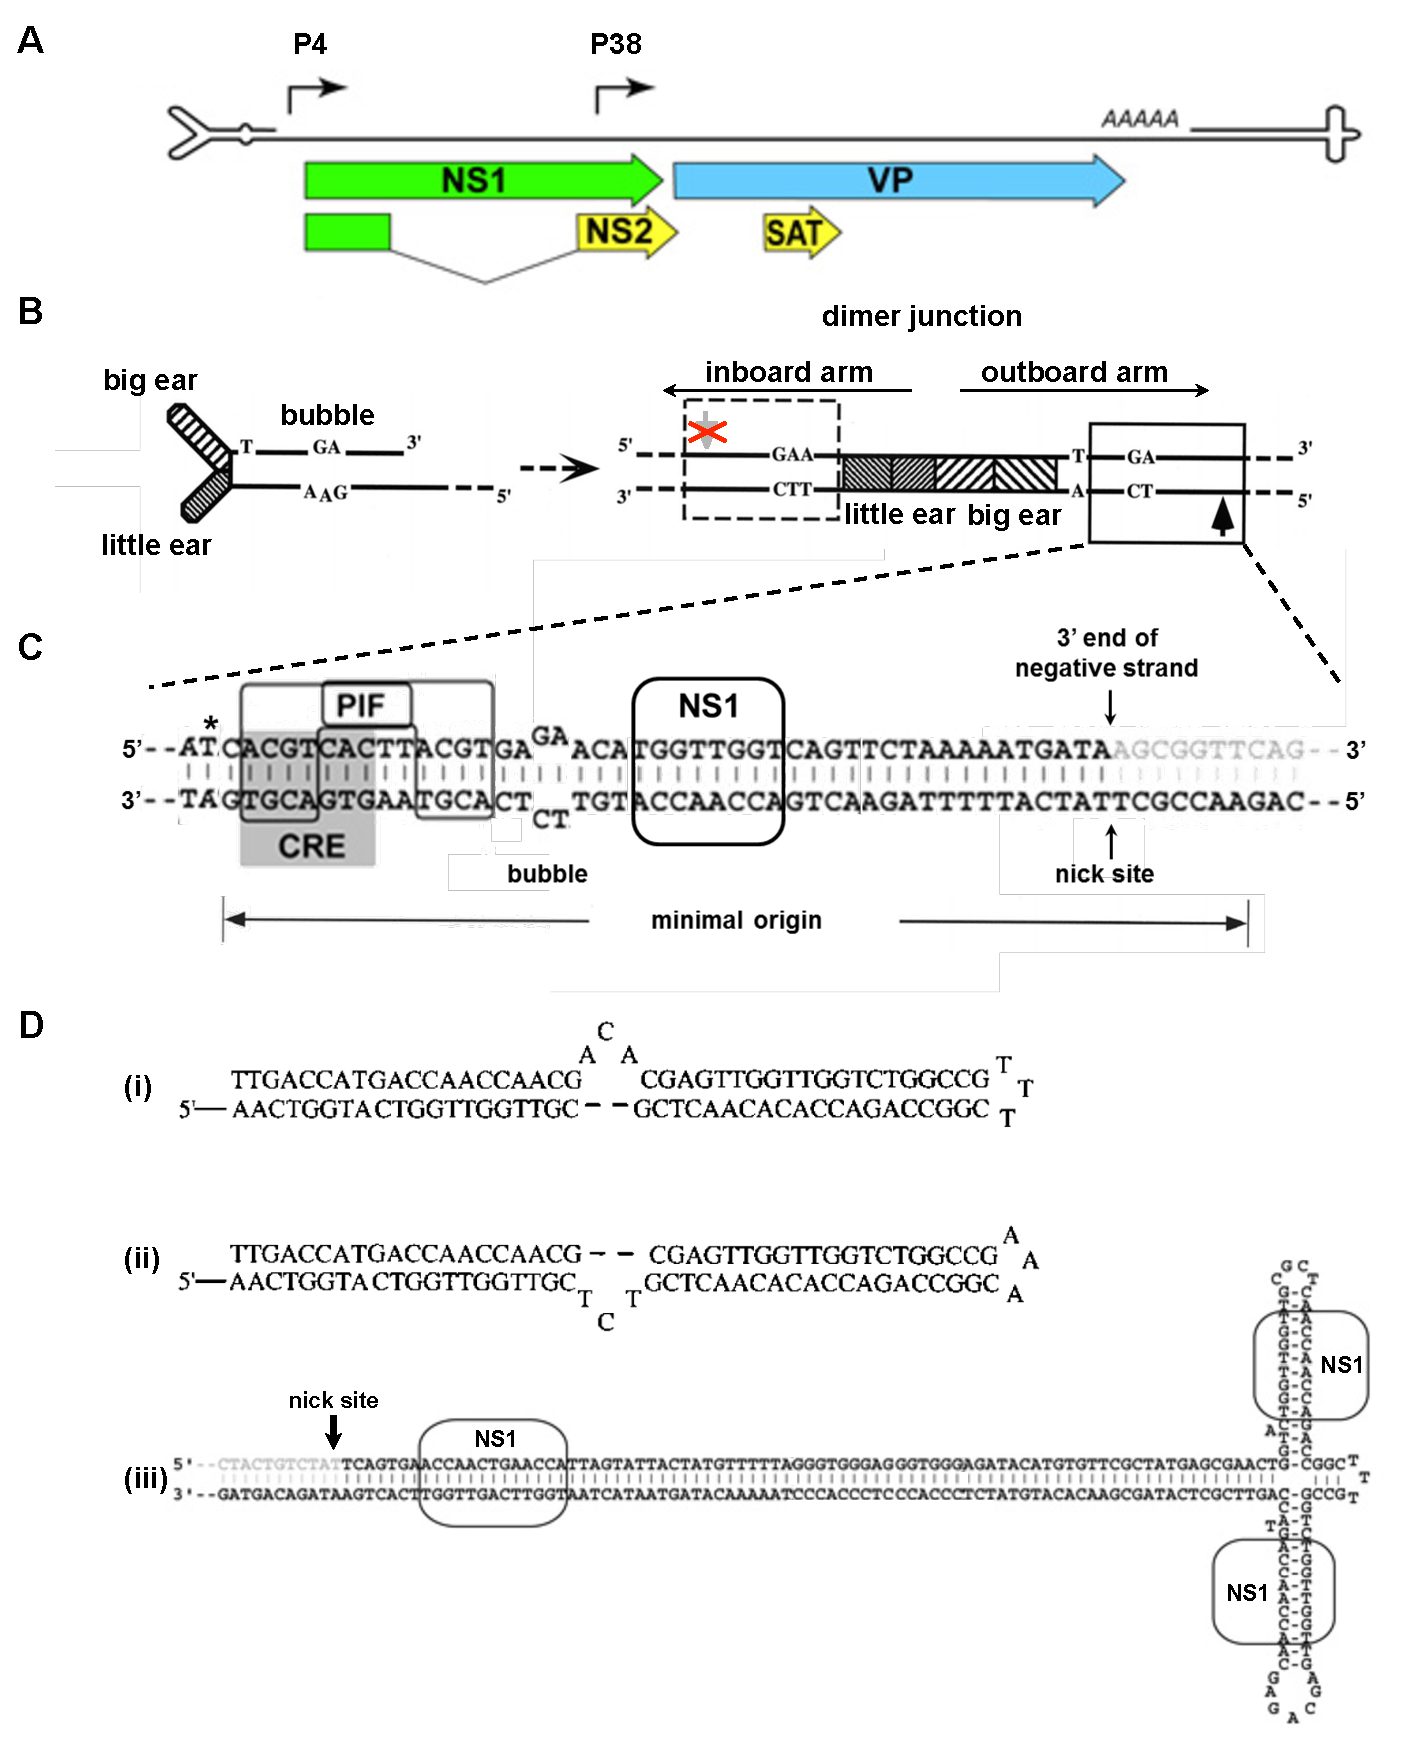
\includegraphics[scale=0.55]{Architecture}
  \caption[Genome architecture of minute virus of mice (MVM).]
   {Genome architecture of MVM. \textbf{(A)} The terminal hairpins, drawn to represent their predicted structures, are scaled approximately 20x relative to the rest of the genome. Major ORFs are represented by arrowed boxes and alternative RNA splicing for NS2 is indicated. Proteins are shaded green for the major replication initiator protein (NS1), blue for the structural (VP) proteins of the capsid, and yellow for sequences unique to the ancillary NS proteins. The two transcriptional promoters, P4 and P38, are indicated by rightward arrows and the polyadenylation site by the AAAAA-sequence block \cite{small}. \textbf{(B)} The left-end hairpin of MVM and the dimer junction are shown in diagrammatic form. Asymmetries, such as the "ear"-like structures, extra-helical T, and bubble sequence are indicated. The fully duplex, dimer junction, generated by RHR (see Section~\ref{Replication}, p.~\pageref{Replication}), is shown on the right hand side. The short, palindromic sequences derived from the hairpin ears are represented by cross-hatched boxes. The active \textit{OriL\textsubscript{TC}} is boxed, with an arrow indicating the nick site. The equivalent sequence generated on the GAA side of the bubble is framed by a dashed box with an arrow at the potential nick site that is crossed out to indicate that \textit{OriL\textsubscript{GAA}} is not active \cite{pmid12885883, pmid16928767}. \textbf{(C)} Sequence details of the active left-end origin (approx. 50 bp) are shown, with an arrow indicating the active nick site. The minimal sequence required for origin activity is indicated by the double-headed arrow. Sequences of the bubble and the PIF, cAMP-responsive element (CRE), and NS1 binding sites are indicated. An asterisk represents the position of the extra-helical T, now base paired, and the gray box below it indicates the CRE consensus sequence \cite{pmid12885883}. \textbf{(D)} Alternate conformations of the right-end hairpin sequences of MVM. The right-end terminus can form a hairpin structure in either the flip (i) of flop (ii) sequence orientation or a cruciform structure (iii). In the cruciform configuration, the binding sites for the replicator protein, NS1, are boxed and their site of nucleolytic cleavage is represented by a vertical arrow \cite{pmid8614999}.
} 
\label{Architecture}
\end{figure}


\nomenclature{VP}{Viral protein}
\nomenclature{NS}{Non-structural (protein)}
\nomenclature{PIF}{Parvovirus initiation factor}
\nomenclature{CRE}{cAMP-responsive element}
\nomenclature{SAT}{Small alternatively translated protein} 
% Chapter 6

\chapter{Host Range and Specificity} % Main chapter title

\label{Chapter6} % For referencing the chapter elsewhere, use \ref{Chapter5} 

% \lhead{Chapter 2. \emph{Methods}} % This is for the header on each page - perhaps a shortened title

%----------------------------------------------------------------------------------------

\section{Tissue Tropism Determinants}

Concerning their host range, most parvoviruses, such as MVM, \nomenclature{MVM}{Minute virus of mice} CPV, \nomenclature{CPV}{Canine parvovirus} and FPV, \nomenclature{FPV}{Feline parvovirus} are tightly restricted to specific receptors of their particular hosts. However, some parvoviruses, as for example many of the AAVs, \nomenclature{AAV}{Adeno-associated virus} infect human cells by primary attachment to a variety of receptors (see Section~\ref{Binding}, p.~\pageref{Binding}). 

As outlined in Chapter~\ref{sec:Discovery and brief history} (see p.~\pageref{sec:Discovery and brief history}), two distinct strains of the parvovirus MVM have been described to occur in mice. On the one hand, MVMp, \nomenclature{MVMp}{Prototype strain of MVM} the prototype strain, replicates efficiently in mouse fibroblasts \cite{pmid5945715}. On the other hand, MVMi,\nomenclature{MVMi}{Immunosuppressive strain of MVM} the immunosuppressive strain, replicates in T lymphocytes \cite{pmid1244418, pmid6264106}.
Both strains display disparate \textit{in vitro} tropism and \textit{in vivo} pathogenicity despite differing by only 14 amino acids in their capsid proteins \cite{pmid1871965}, thus providing a useful model for in-depth characterization of the role of virus-receptor interaction (see Section~\ref{Binding}, p.~\pageref{Binding}) in parvovirus infection. Beyond that, MVMp and MVMi are serologically indistinguishable, bind to sialic acid, and are internalized in both fibroblasts and lymphocytes \cite{pmid6602221}. Consequently, it could be demonstrated that both viruses propagate in hybrids of the two cell types \cite{pmid6602222}.    

In order to map the allotropic determinants of MVM, chimeric viral genomes were constructed \textit{in vitro} from infectious genomic clones of both strains. By mutagenesis and selective plaque assays, the major determinants for the acquisition of fibrotropism for MVMi have been mapped onto the capsid \cite{pmid3257270, pmid9519837, pmid1871965}, in particular to the VP2 residues 317 and 321 \cite{pmid7637028, pmid1316457}. Both residues are located at the base of the threefold spike of the virion \cite{pmid3357208, pmid3392768, pmid3257270}. Interestingly, these two VP2 residues structurally localize nearby some of the important amino acids determining CPV, FPV, and PPV host range \cite{pmid14581558, pmid12941920, pmid1532105}. Further residues (VP2 residues 339, 399, 460, 553, and 558) were identified in MVMi to be able to confer fibrotropism to forward second-site mutants when either residues 317 or 321 are mutated. Those residues cluster around the twofold dimple-like depression \cite{pmid9817841}. In contrast, the switch to lymphotropism for MVMp is more complex and requires both an equivalent region of the major MVMi capsid protein gene VP2 and a segment of the non-structural protein genes \cite{pmid9519837}.    


\section{Pathogenicity Determinants}

MVMi appears to be more pathogenic in mice than MVMp. Oronasal inoculation of MVMi in most neonatal mice resulted in lethal phenotype or severe growth-retardation in survivors \cite{pmid3712557}, as observed for other parvoviruses (see Section~\ref{sec: The Parvovirinae subfamily}, p.~\pageref{sec: The Parvovirinae subfamily}). MVMp infection appears to be asymptomatic in newborn mice \cite{pmid1373202}. In contrast, MVMi infection in neonatal mice of some inbred strains caused renal papillary hemorrhage and viral replication in endothelia \cite{pmid1653878}, hematopoietic precursors \cite{pmid7707557}, and neuroblasts \cite{pmid8892936}. Following \textit{in utero} inoculation of MVMi or MVMp into developing embryo, a broad set of cell types were infected that partially overlapped. Nevertheless, the tissue tropism of MVMp for fibroblasts and of MVMi for endothelium, as well as the higher virulence of MVMi was preserved \cite{pmid15308740}. 
By reason of the complexity of MVMi pathogenesis in the neonatal mouse, a more adequate model was required to investigate the virulence of MVMi \textit{in vivo}. 

Severe combined immunodeficiency (SCID) mice \cite{pmid6823332} represent such a model since they lack an antigen-specific immune response, thus allowing the study in adult mice and circumventing the complex situation of heterogenous viral multiplication in embryonic developing tissue. MVMi infection of adult SCID mice gave rise to the suppression of long-term repopulating hemopoietic stem cells in the bone marrow \cite{pmid12857918}, leading to an acute lethal leukopenia and accelerated erythropoiesis \cite{pmid9971754}.
In addition, it has been reported that MVMp evolved in intravenously inoculated SCID mice. Different variants, isolated from single plaques, carried only one of three single amino acid changes at position 325, 362, or 368 in the major VP2 capsid protein. These variants sustained their fibrotropism \textit{in vitro}, but unlike MVMp, they propagated in mouse tissues following oronasal inoculation, eventually causing death \cite{pmid16415031, pmid16103180}.
Two of the three invasive fibrotropic MVMp strains, I362S and I368R, were shown to induce lethal leukopenia in oronasal inoculated SCID mice. Emerging viral populations in leukopenic mice displayed altered sequences in the MVMi genotype at position 321 and 551 of VP2 for infections with the I362S variant or changes at position 551 and 575 in the K368R virus infections. In general, a high level of genomic heterogeneity in the DNA sequence encoding the VP2 protein was observed and was found to be clustered at the twofold depression of the viral capsid \cite{pmid18045943}.            	
	
	
\section{Comparison of Tissue Tropism and Pathogenicity Determinants among Parvoviurses}	
	
	Significantly, the amino acids dictating \textit{in vitro} tropism (317 and 321), \textit{in vivo} pathogenicity (325, 362, and 368), fibrotropism on MVMi (339, 399, 460, 553, and 558), and those involved in the development of leukopenia (321, 551, and 575) were found to be located on, or near the capsid surface. Structurally, these residues cluster mainly by raised elements around the twofold axes of symmetry, in close vicinity of the sialic acid binding pocket (see Section~\ref{Binding}, p.~\pageref{Binding}) \cite{pmid16415031, pmid18045943}.   
	
Differences in the tissue tropisms and the pathogenic phenotypes  have also been mapped to the capsid proteins of Aleutian mink disease parvovirus \cite{pmid8396664}, porcine parvovirus (PPV) \nomenclature{PPV}{Porcine parvovirus} \cite{pmid8642680}, CPV \cite{pmid3176341, pmid1331498}, and FPV \cite{pmid7513918} in a capsid region analogous to that observed for MVM (reviewed in \cite{tropism}). These pronounced \textit{in vitro} tropism and \textit{in vivo} pathogenicity disparities between the highly homologous viruses can occur at any of the various stages of the infectious viral life cycle, including cell receptor binding, internalization, capsid uncoating, DNA replication or transcription. Studies of the strain-specific tissue tropism conducted on members of other virus families have mainly shown that each strain recognizes a different specific cell surface receptor \cite{pmid6290894, pmid13908368, pmid6293181, pmid6278730, pmid7436739, pmid7365250, pmid271999}. This receptor is only present on the target cell for that strain, but absent on the surface of other potential host cells. Although the same structural elements of parvoviruses are involved in mediating host and tissue tropisms, each appears to be affecting a different mechanism. Host ranges of CPV and FPV are controlled by receptor binding, as observed for many other viruses, whereas the cell tropisms of MVM appear to be due to restrictions of interactions with intracellular factors \cite{pmid9817841, pmid12941411, pmid6602221}. For MVM it was suggested that the point of restriction appeared after nuclear targeting and conversion of genomic ssDNA to RF intermediates but prior to viral genome replication. Most likely, the restraint occurs due to a block in capsid uncoating \cite{pmid9311862, pmid1322591}.

As discussed in this section the functional regions among the subfamily \textit{Parvovirinae} co-localize to similar capsid surface regions albeit three general parvovirus topology groups with characteristic local morphological surface differences emerged (see Chapter~\ref{sec:Morphology}, p.~\pageref{sec:Morphology}). A profound understanding of functional domains that are involved in fundamental steps of the viral life cycle, particularly receptor attachment, \textit{in vitro} tropism, \textit{in vivo} pathogenicity, and antigenicity are essential for infection and disease control. Hence, showing great promise to allow genetic engineering of parvovirus capsids for the therapeutic delivery to be controlled or modified in gene therapy applications and to develop foreign antigens \cite{pmid12941411, tropism}.
\label{Chaper6end}     



%Although MVMi infection may result in pathology of infected mice, it has been shown that the infection more likely interferes with numerous T-cell functions \textit{in vitro}. The infection rather causes problems for the ongoing study the mice are being used for as the immune system will be activated, the activity of T-lymphocytes or B-lymphocytes will be altered and tumor formation may be suppressed \cite{pmid6457871, pmid6264106, pmid11528091}.

\nomenclature{SCID}{Severe combined immunodeficiency}
\nomenclature{RF}{Replicative form} 
% Chapter 7

\chapter{The Parvovirus Life Cycle} % Main chapter title

\label{Chapter7} % For referencing the chapter elsewhere, use \ref{Chapter2} 

% \lhead{Chapter 2. \emph{Methods}} % This is for the header on each page - perhaps a shortened title

%----------------------------------------------------------------------------------------
As previously mentioned, parvoviruses are heavily dependent on their cellular systems to ensure productive infection. A plethora of molecular interactions between the virus and the host cell allow the recruitment of cellular machinery to provide an environment for optimal progeny morphogenesis. These numerous interactions include binding to the cell surface determining primary attachment and internalization, cytoplasmic interactions controlling intracellular trafficking and eventual maturation, and nuclear interactions regulating uncoating, replication, transcription, assembly, and packaging of progeny particles. Some of the viral mechanisms and interactions underlying the parvovirus life cycle are introduced in this chapter in further detail keeping MVM as the main focus.     


\begin{figure}[H]
\centering
  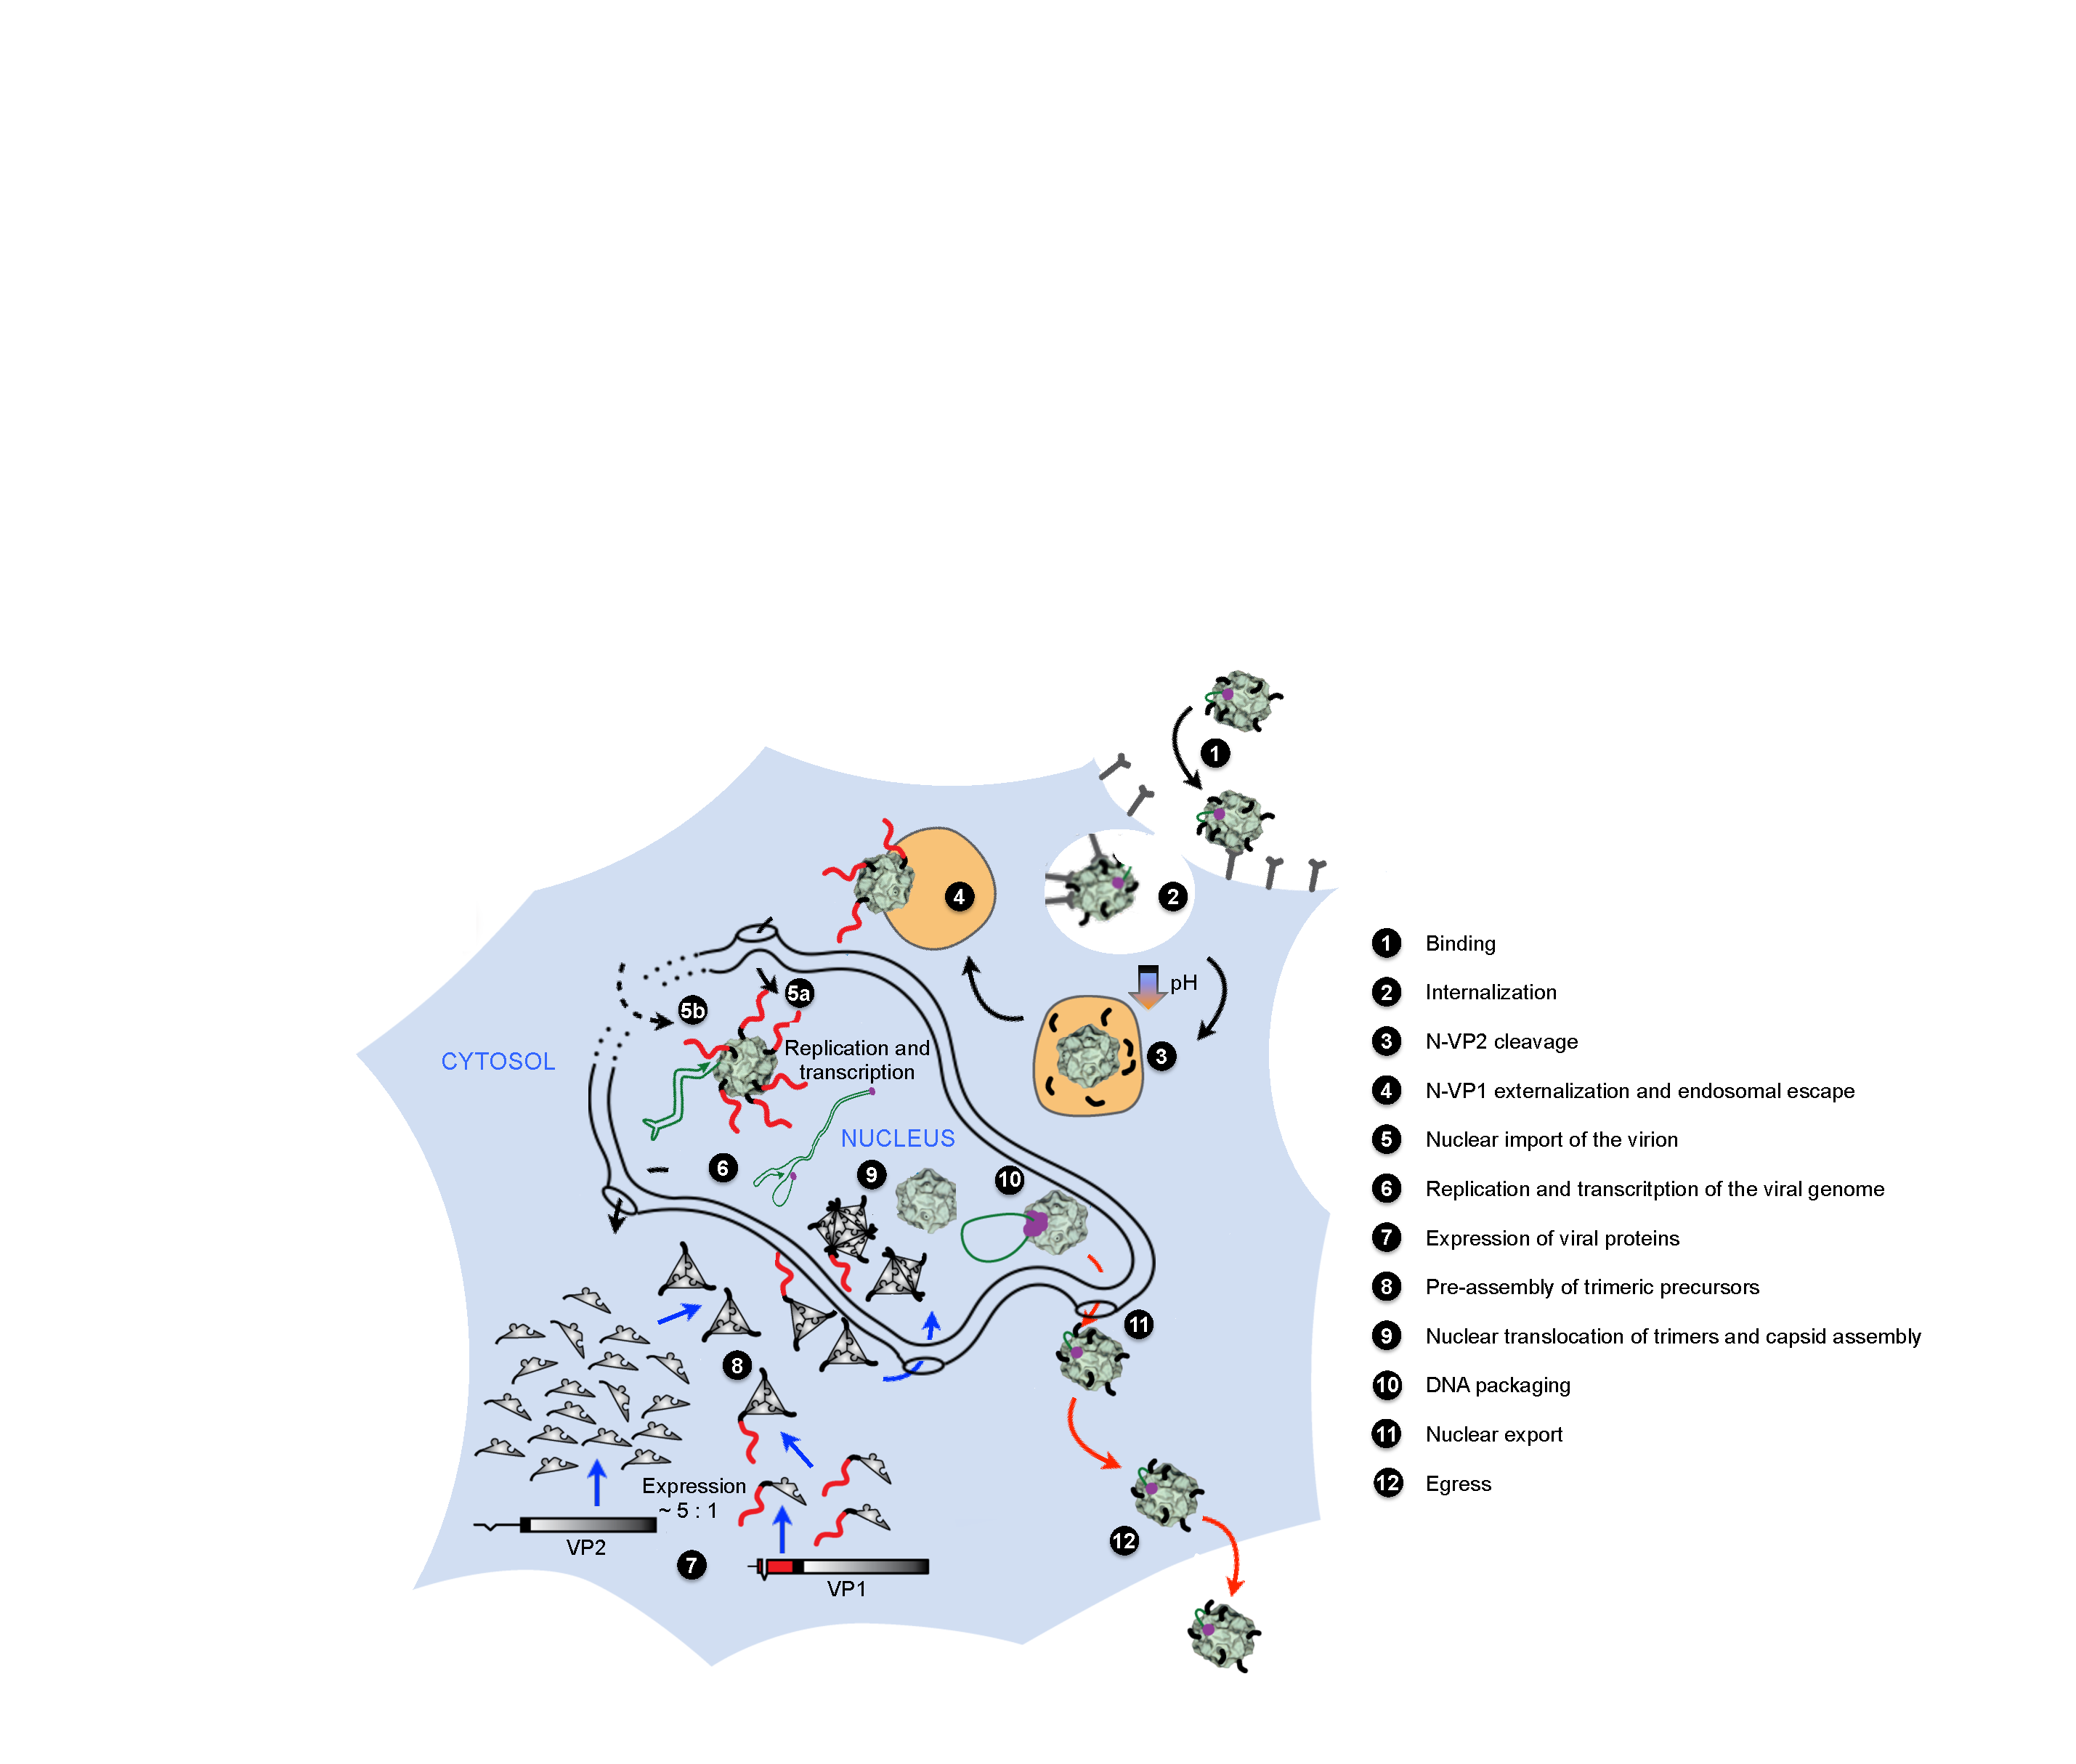
\includegraphics[scale=0.35]{Cycle}
  \caption[Life cycle of MVM]
   {Simplistic view of the life cycle of MVM. Cell entry (black arrows), protein expression and progeny assembly (blue arrows), and DNA packaging, nuclear export and egress (red arrows) are illustrated. The unknown sialylated cell surface receptors are indicated as extended Y shapes and acidic late endocytic vesicles are colored in orange. Colored lines associated with virus particles represent the flexible N-VP2 termini (black), the VP1u region (red), and the viral genomic DNA (green). The number of externalized N-VP1 termini is not known and might vary between one and ten. Currently, nuclear targeting (step 5) of the virion is controversial and remains unclear. Due to its small size, MVM could physically traverse the nuclear pore complex (NPC) fully intact (step 5a). Alternatively, MVM was suggested to enter the nucleus in an NPC-independent manner by partial disruption of the nuclear envelope (step 5b). Horizontal bars represent primary VP gene transcripts and jigsaw triangles indicate the folded core containing the jellyroll motif common to all VP polypeptides. The multifunctional NS1 protein, which assists DNA replication and packaging, is represented as purple sphere. This schematic representation is not drawn to scale and was adapted from reference \cite{small}.  
} 
\label{Cycle}
\end{figure}


\section{Receptor Binding}
\label{Binding}
Recognition of cell surface receptors by a virus enables the first step of infection and hence, represents a key parameter of tropism and pathogenesis (see Chapter~\ref{Chapter5}, p.~\pageref{Chapter5}). Different biomolecules, such as proteins, carbohydrates, and glycolipids can serve as primary attachment factors. To date, a variety of different receptor molecules with specific binding properties or functional activities have been identified for some members of the subfamily~\textit{Parvovirinae} (see Table~\ref{Tab: Receptors}, p.~\pageref{Tab: Receptors}. For a review see reference \cite{Receptor}). Examples include the AMDV-binding protein for AMDV \cite{pmid10196278}, the globoside erythrocyte P antigen, along with $\alpha$\textsubscript{5}$\beta$\textsubscript{1}-integrin and Ku80 for B19V \cite{pmid8211117, pmid15661151, pmid12907437, pmid16076874, weigel}, transferrin receptors (TfRs) for CPV, FPV and mink enteritis virus \cite{pmid16040076, pmid11264378} and heparan sulfate proteoglycan (HSPG), $\alpha$\textsubscript{\RM{5}}$\beta$\textsubscript{5}-integrin, and growth factor receptors for AAVs \cite{pmid14502277, pmid15596854, pmid9883842, pmid9445046, pmid9883843, pmid8599196}. However, a recent study from our lab conducted on B19V failed to verify the interaction between B19V and $\alpha$\textsubscript{5}$\beta$\textsubscript{1}-integrin. Instead, purified, recombinant VP1u was demonstrated to bind and internalize independently of the B19V capsid. VP1u binding and internalization was tightly restricted to only a few cell lines of the erythroid cell lineage only. These results, together with the ability of recombinantly expressed VP1u to efficiently prevent B19V endocytosis, indicate that an unknown receptor with an expression pattern confined to few erythroid cell types mediates B19V internalization \cite{pmid24067971}.  

For most of the parvoviruses only the glycan component of their specific receptor is known. Glycans are carbohydrate polymers and represent the major components of the cell surface. Thus they provide a vast collection of important cellular attachment factors for viruses in general. They may be conjugated with cell surface proteins or membrane lipid head groups to form glycoproteins and glycolipids, respectively, or constitute glycosaminoglycan chains attached to proteoglycans \cite{pmid16019714}. The extensive heterogeneity of the carbohydrate polymers which are expressed across different species, and even across different tissues within the same species, creates an immense variability in viral tissue tropism. This diversity is even further enlarged by various glycosidic linkage positions between each individual monosaccharide and by the high degree of chemical modifications of hydroxyl groups \cite{pmid11841250, pmid17632542}. Most commonly, SA or sulfated oligosaccharide motifs of glycosaminoglycans (e.g. heparan sulfate) form the distal and hence most surface exposed units of glycoepitopes \cite{pmid17072005}.


Biochemical studies utilizing neuraminidase and proteinase K treatment have shown that SA is a common primary attachment factor for several parvoviruses infecting different species, as for example MVM \cite{pmid3296697, pmid16415031}, parvovirus H1 (H1-PV) \cite{pmid22258256}, BPV \cite{pmid15750863, pmid9747725, pmid15269359}, PPV \cite{pmid20484503}, AAV1 \cite{pmid16943302, pmid16940521}, AAV4, AAV 5 \cite{pmid15761263, pmid11435568, pmid11262413, pmid16409121}, CPV and FPV \cite{pmid1329321, pmid7975239}. However, SA-CPV and SA-FPV interactions are not sufficient for infectivity but require additional binding to their respective TfRs on canine and feline cells \cite{pmid1329321, pmid12525605, pmid11264378, pmid12885908}. More than 60 analogues of SA occur in nature which result from modifications to the nine-carbon backbone \cite{pmid17072005} and are estimated to be present at 5~$\times$~10\textsuperscript{5} copies per cell on A9 mouse fibroblasts \cite{pmid20517, pmid6602221}. The SA binding pocket of MVM was identified by analysis of SA soaked into preformed crystals of virus-like particles (VLPs)\footnotemark of MVMp. Structurally, the SA electron density is associated with the dimple-like depression located at the icosahedral two-fold axis in the MVM cpasid (see Figure~\ref{Morphology}, p.~\pageref{Morphology}). The binding pocket exposes highly positive charges which interact with SA moieties on the cell surface \cite{pmid16415031}. Interestingly, the localization of the SA binding domain in MVM is proximal to the CPV and FPV determinants of SA binding to erythrocytes \cite{pmid7645206, pmid8392729, pmid1329321, pmid10884355}. Significantly, the amino acids determining \textit{in vitro} tropism (317 and 321) and \textit{in vivo} pathogenicity (325, 362, and 368) for MVM invariably localize in close vicinity of the SA binding pocket (see Chapter~\ref{Chapter5}, p.~\pageref{Chapter5}) \cite{pmid16103145}.                  

The identification of virus receptors and the characterization of virus-receptor interactions are of great relevance for understanding virus evolution, host tropism, and pathogenesis. A profound knowledge of the first steps of viral infections on the host cell surface is essential for the development of antiviral therapies and for the construction of gene therapy vectors with determined targeting.    


\footnotetext{VLPs are non-infectious particles which do not contain any viral genetic material. The expression of parvoviral structural proteins results in a spontaneous self-assembly of VLPs. Since VLPs mimic the organization and conformation of viral surface epitopes, they can elicit strong B cell and T cell immune responses. Therefore, they provide a useful tool for the development of vaccines.}

\begin{small}
\begin{center}

\begin{longtable}{P{0.7in} P{1.65in} P{1.45in} P{0.6in} P{0.8in}}
\caption[Parvoviruses and their receptors]{\normalsize Parvoviruses and their receptors}\\
\\
\label{Tab: Receptors}
\normalsize\textbf{Virus} & \normalsize\textbf{Receptor} & \normalsize\textbf{Coreceptor} & \normalsize\textbf{Host} & \normalsize\textbf{Reference}\\
\hline
\endfirsthead % all the lines above this will be repeated on every page

\multicolumn{3}{l}{\normalsize\textbf{Table~\ref{Tab: Receptors}} continued}\\
\\
\normalsize\textbf{Virus} & \normalsize\textbf{Receptor} & \normalsize\textbf{Coreceptor} & \normalsize\textbf{Host} & \normalsize\textbf{Reference}\\
\hline
\endhead

\hline
\multicolumn{5}{l}{This Table was adapted from reference \cite{Halder}}
\endlastfoot

AAV1 & $\alpha$2-3 and $\alpha$2-6 N-linked SA & - & Human & \cite{pmid16940521} \\
AAV2 & HSPG & Integrin $\alpha$\textsubscript{5}$\beta$\textsubscript{1}, $\alpha$\textsubscript{\RM{5}}$\beta$\textsubscript{5}, FGFR1, HGFR, LamR & Human & \cite{pmid16973587, pmid15596854, pmid9883842, pmid9883843, pmid9445046, pmid16940508} \\
AAV3 & HSPG & HGFR, LamR, FGFR1 & Human & \cite{pmid16973587, pmid20545554, pmid16195782} \\
AAV4 & $\alpha$2-3 O-linked SA & - & NHP & \cite{pmid11435568} \\
AAV5 & $\alpha$2-3 and $\alpha$2-6 N-linked SA & PDGFR & Human & \cite{pmid14502277, pmid16409121, pmid11262413, pmid11435568} \\   
AAV6 & $\alpha$2-3 and $\alpha$2-6 N-linked SA, HSPG & EGFR & Human & \cite{pmid20473307, pmid16940521, pmid16943302} \\  
AAV8 & - & LamR & NHP & \cite{pmid16973587} \\
AAV9 & Galactose & LamR & Human & \cite{pmid16973587, pmid21576824, pmid21330365} \\
Bovine AAV & Gangliosides, chitotriose & - & Bovine & \cite{pmid20231878, pmid16699032} \\
AMDV & AMDV-binding protein & - & Mink & \cite{pmid10196278} \\
BPV1 & SA & Glycophorin A & Bovine & \cite{pmid15750863, pmid9747725} \\
B19V & Erythrocyte P antigen & Integrin $\alpha$\textsubscript{5}$\beta$\textsubscript{1}, ku80 & Human & \cite{pmid8211117, pmid15661151, pmid12907437, pmid16076874, weigel} \\
MVM & SA & - & Rodent & \cite{pmid3296697, pmid15229399, pmid16822863} \\
CPV/FPV & SA & TfR & Cat, dog & \cite{pmid11264378, pmid12525605} \\
PPV & SA & - & Swine & \cite{pmid20484503} \\

     
\end{longtable}
\end{center} 
\end{small}


\section{Receptor-mediated Endocytosis}
\label{Endocytosis}
All known parvoviruses enter the host cell by receptor-mediated endocytosis, using a wide variety of partially unknown glycosylated receptor molecules, exposed on the cell surface \cite{pmid18406140} (see Table~\ref{Tab: Receptors}, p.~\pageref{Tab: Receptors}). The endocytic route is advantageous for karyophilic viruses. On the one hand, endosomes provide a rapid and efficient transport towards the nuclear periphery. On the other hand, the exposure to low pH enables the capsid to undergo conformational changes which are required for further stages of infection (see Section~\ref{Rearrangements}, p.~\pageref{Rearrangements}), such as endosomal escape, uncoating, and nuclear localization. Recent research has demonstrated that, in addition to the classical clathrin-mediated endocytosis \cite{pmid20484503, pmid10559355, pmid10644365}, several alternative endocytic routes can be used by parvoviruses. For example, AAV2 utilizes clathrin-independent carriers (CLICs) \cite{pmid22177561}, AAV5 uses caveolae-dependent endocytosis \cite{pmid19141440}, and PPV utilizes macropinocytosis \cite{pmid20484503} as additional endocytic pathways. Most recently, Garcin and Panté showed that MVM enters its host cell by at least three potential endocytic routes. Inhibition of various endocytic pathways with specific drugs in combination with EM, immunofluorescence microscopy (IF), and fluorescence-activated cell sorting, identified clathrin-, caveolin-, and CLIC-mediated endocytosis for MVM. However, the latter endocytic uptake mechanism was restricted to transformed cells only, but did not occur in murine A9 fibroblasts. This observation was confirmed in further experiments which demonstrated that dynasore, an inhibitor of dynamins, completely blocked MVMp uptake in A9 mouse fibroblasts, whereas its inhibitory effect was incomplete in transformed cells. These results indicate that both clathrin- and caveolin-mediated MVMp endocytosis is dependent on dynamin in murine A9 fibroblasts, but transformed cells allow for the dynamin-independent CLIC-mediated uptake of MVMp \cite{pmid25863880}. Although parvoviruses share some general features in receptor binding and in their routes of cellular entry, each appears to display their own unique mechanistic details.     

\section{Endosomal Trafficking and Capsid Rearrangements}
\label{Rearrangements}
Endosomal trafficking of parvovirus virions is thought to be a slow and rate-limiting process in viral infection \cite{pmid10841516, pmid10623762, pmid11287557, pmid16379002}. The delayed progression to infection allows parvoviruses the opportunity to undergo important structural transitions and prolonged processing within endosomes. For instance, AAVs escape from early endosomes but only reach the nucleus after 40 min to 2 hours post-infection (hpi) \cite{pmid10684294, pmid12388712}. MVM is exceptionally well characterized with respect to endosomal trafficking in spite of the rapid dynamics and complexity of viral movement within and between endosomal compartments. It has been reported to traffic even slower through the endocytic pathway and only reaches the cell nucleus after 8 hpi when DNA replication was detected \cite{pmid12438589}.       

Several lines of evidence confirm that endosomal processing of incoming parvovirus particles is essential. First, virions with or without exposed N-VP2 termini failed to confer a nuclear localization phenotype to AAV2 when directly injected into the cytoplasm to bypass the endocytic pathway \cite{pmid16956943, pmid15829993}. Similarly, low pH pre-treated CPV capsids were unable to accumulate in the nucleus following injection into the cytoplasm \cite{pmid9420290}. Also, for MVM all structural rearrangements were equally impaired by lysosomotropic drugs, thereby preventing infection \cite{pmid16379002, pmid12438589}. These drugs, such as bafilomycin A\textsubscript{1} or the weak base chloroquine diphosphate, raise the endosomal pH by inhibiting the vacuolar-type H\textsuperscript{+}-adenosine triphosphatase (ATPase) \cite{pmid2973058, pmid6094416, BafA1} or by accumulation inside acidic compartments \cite{pmid4606365, pmid28524, pmid6169733}, respectively. Finally, endosomal acidification has been demonstrated to be essential for the infection of AAV \cite{pmid10684294, pmid15681453, pmid11160681, pmid11287557}, CPV \cite{pmid10644365, pmid9420290, pmid1733094}, and MVM \cite{pmid16379002, pmid12438589}.  


Already 30 min after endocytosis, three considerable structural rearrangements of the MVM capsid occurred simultaneously. Specifically, the capsid transitions include the cleavage of the exposed N-VP2 termini, the externalization of originally sequestered N-VP1 termini, and the release of the full-length viral DNA genome without the loss of capsid integrity \cite{pmid16379002}. The conformational changes of parvovirus capsids, which are induced by endosomal trafficking \textit{in vivo}, can be partially mimicked \textit{in vitro}. Treatment of CPV particles under acidic conditions mimicking endosomal pH induced VP1u exposure \cite{pmid14644609}. However, in the case of MVM full capsids (FC), prior cleavage of N-VP2 termini to VP3 is a prerequisite for VP1u externalization under such conditions \cite{pmid9927584, pmid16352540}. Contrarily, the N-VP2 termini remained buried in the interior of ECs and thus they were not accessible to proteolytic digestion \cite{pmid16379002}. Surprisingly, EC exposed the N-VP1 termini with similar kinetics to FC, indicating that at least for EC, neither the genomic DNA nor the cleavage of N-VP2 is involved in the extrusion of N-VP1 \cite{pmid9927584, pmid16379002}. Harsh conditions, such as exposure to heat or urea, trigger VP1u externalization in AAV \cite{pmid15827144}, CPV \cite{pmid11799183, pmid9770425}, and MVM particles \cite{pmid9927584, pmid19955311}. Characterization of the biochemical and structural capsid dynamics was enabled by artificial \textit{in vitro} treatments although they cannot directly reproduce physiological conditions \cite{pmid9927584, pmid19955311, pmid15827144, pmid11799183}. The differences observed in the \textit{in vitro} and \textit{in vivo} studies imply that a combination of several factors, such as receptor binding, low endosomal pH, or interactions with unknown host factors play a role in these structural transitions of parvoviruses.       

The study of the infectious pathway of parvoviruses is impeded by the fact that the bulk of incoming particles are retained within lysosomal compartments and only a minority escapes the endocytic route (see Section~\ref{Escape}, p.~\pageref{Escape}). Moreover, the lack of dynamic information in fixed cell samples has complicated the examination of virus trafficking through the highly dynamic and overlapping vesicular endocytic pathway. However, emerging advances in time-lapse microscopy make live-cell imaging an important complementary method to study the complex nature of endosomal trafficking in the future.

\nomenclature{ATPase}{Adenosine triphosphatase}
\nomenclature{ATP}{Adenosine triphosphate}

\section{Endosomal Escape}
\label{Escape}
The high particle to infection (P/I) ratio\footnotemark of most parvoviruses (100:1 to >1000:1) \cite{pmid4673484, pmid20649475, pmid7288919} indicates that most of the incoming viruses fail to enter the nucleus. Indeed, a substantial portion of the incoming MVM virions was demonstrated to follow a non-infectious pathway ending up in lysosomal compartments where they co-localized with co-endocytosed dextrans which had a MW of 10 kDa and were used as lysosomal marker. Hence, the endosomal escape represents the major barrier for the subsequent steps of MVM infection. However, the inability to escape from the endocytic route was not due to a failure in endosomal processing of MVM since all virions retained in lysosomal compartments underwent the required structural transitions. MVM VLPs or ECs that accumulated in lysosomes remained intact up to 50 hpi but the exposed, capsid-tethered viral DNA of FCs was degraded 21 hpi, most probably, by the lysosomal endonuclease DNase~\RM{2} activity \cite{pmid16379002}. \footnotetext{The P/I ratio is the number of virus particles per plaque-forming unit (PFU).}

Unlike enveloped viruses, non-enveloped viruses are unable to deliver their genomes into the host cell by fusion with the cellular plasma or endosomal membrane \cite{pmid18596815}. They must employ alternative strategies to breach their host cell's delimiting membrane. Although MVM has not yet been directly demonstrated to permeabilize endosomal membranes, there is evidence that parvoviruses have the capability to disrupt membranes. Labeled dextrans with a MW of 3 kDa were progressively liberated into the cytosol 8-20 h after co-endocytosis with CPV virions. However, despite the apparent change in the permeability of endosomal membranes, there is no complete disintegration of endosomal vesicles since larger dextrans with a MW of 10 kDa, as well as $\alpha$-sarcin, were mainly retained in vesicles at the same time post-infection \cite{pmid14644609, pmid10644365}.

Several arguments speak in favor of the N-VP1 terminal PLA\textsubscript{2} activity (see Section~\ref{PLA2}, p.~\pageref{PLA2}) mediating endosomal escape of parvoviruses. Firstly, N-VP1 becomes exposed in early endocytic vesicles \cite{pmid16379002, pmid14644609, pmid9927584, pmid16284249, pmid11961250, pmid20974479, pmid11702787}. Secondly, VP1 has been demonstrated to be essential for productive infection of parvoviruses in a step prior to the initiation of DNA replication \cite{pmid8416366, pmid10684294, pmid1733094, pmid11160681, pmid11287557, pmid10644365, pmid12438589, pmid9420290}. Lastly, pre-incubation of N-VP1-exposing CPV virions with PLA\textsubscript{2} inhibitors, such as quinacrine and manoalide, significantly reduced or completely abolished infectivity, respectively \cite{pmid14644609}. For MVM \cite{pmid16284249} and AAV2 \cite{pmid20974479}, complementation assays between wild-type and mutant particles have been used to demonstrate that the lipolytic PLA\textsubscript{2} function is mediating phospholipid bilayer penetration. Accordingly, mutants with amino acid substitutions within their catalytic dyad (see Section~\ref{PLA2}, p.~\pageref{PLA2}) were constructed. Their enzymatic activity was severely impaired and viral infectivity was completely abrogated. Polyethyleneimine-induced endosomal rupture or co-infection with wild-type or mutant virions could partially rescue the mutant phenotype. Similarly, co-infection with endosomolytically active adenoviral variants resulted in a partial complementation of the mutant phenotype. Contrarily, endosomolytically inactive adenoviral variants, as well as wild-type ECs carrying sequestered VP1u sequences, were unable to restore infectivity of the PLA\textsubscript{2}-negative mutants. Thus, the capsid-tethered PLA\textsubscript{2} motif seems to be either directly or indirectly required for successful penetration of the endosomal membranes.  

Information about the site of endosomal escape for MVM is still lacking. Previous \textit{in vitro} experiments showed that the optimal pH for the parvoviral PLA\textsubscript{2} enzymatic activity ranges between pH 6 to 7, but drastically decreases at a pH below 5 \cite{pmid14726513}. Correspondingly, the acidic, lysosomal environment would not provide optimal conditions for PLA\textsubscript{2}-mediated escape from the degradative pathway. Therefore, it is tempting to speculate that only a few viruses manage to escape the endocytic route from a pre-lysosomal compartment in the absence of vesicle disintegration. This hypothesis is supported by the fact that MVM externalizes N-VP1 already within the first minutes of infection, thus exposing the functional PLA\textsubscript{2} enzymatic activity on its surface. Additionally, brefeldin A, a fungal antibiotic that blocks the transition between early and late endosomes \cite{pmid1682055}, has been demonstrated to abrogate MVM infection \cite{pmid12438589}. In summary, these results collectively suggest that the minority of virions that enter the cytosol escape from an intermediate pre-lysosomal vesicle, namely late endosomes \cite{pmid16379002}.

%Endosomal escape might be heavily restricted because the endocytic route is highly dynamic, showing significant differences in pH, and virions must undergo all required structural transitions within a tight time frame. Accordingly, successful escape only occurs if both requirements are fully accomplished.      

    
\section{Cytosolic Trafficking and Interactions with the Proteasome}
Free diffusion of macromolecular complexes, such as viruses, is strictly limited in the lattice-like mesh of actin microfilaments, intermediate filaments, and microtubules present in the cytoplasm \cite{pmid10553280, pmid9214387}. Karyophilic viruses require active transport through the cytoplasm in order to reach the perinuclear area. CPV has been demonstrated to depend on active, dynein-mediated retrograde transport along the microtubules. Nocodazole (ND), a highly specific antimicrotubular drug promoting tubulin depolymerization in mammalian cells, prevented nuclear translocation of CPV. Similarly, an antibody against the intermediate chain of the motor protein dynein also reduced the nuclear accumulation of CPV capsids. EM based studies and co-immunoprecipitations (IPs) of CPV with the intermediate chain of dynein reinforced a dynein-mediated transport of CPV along the microtubules toward the nucleus \cite{pmid12970411, pmid11932407, pmid10775624}. For MVM similar observations were reported. Intracellular transport requires a functional cytoskeleton and particularly depends on both microfilaments and microtubules. Both compounds cytochalasin D (CD), a drug inhibiting actin filament function, and ND had a moderate decreasing effect on nuclear viral DNA amplification \cite{pmid12438589}.  


Parvoviruses likely undergo further processing in the cytoplasm because microinjection of virions with or without externalized N-termini did not confer a nuclear translocation phenotype \cite{pmid10644365, pmid16956943, pmid14644609, pmid11932407}. For AAV2 and AAV5 it has been demonstrated that phosphorylation of surface exposed tyrosine residues followed by ubiquitination targets viral capsids for proteosomal degradation \cite{pmid11836382, pmid18834608, pmid18511559}. Correspondingly, co-administration of proteasome inhibitors, such as e.g. the tripeptidyl aldehyde MG-132, enhances AAV2 and AAV5 transduction efficiency. In contrast, proteasome inhibition was detrimental to infection for the autonomous parvoviruses PPV, CPV, and MVM. In particular, the chymotrypsin-like activity of the proteasome appeared to be essential for infection. While PPV capsid proteins were ubiquitinated early during the course of infection, no particle ubiquitinylation or degradation was observed for CPV and MVM \cite{pmid20484503, pmid12438589, pmid15207621}.

\nomenclature{CD}{Cytochalasin D}
\nomenclature{ND}{Nocodazole}




\section{Nuclear Targeting}
\label{Localization}      
In addition to the plasma membrane, the nuclear envelope constitutes a second barrier to karyophilic viruses. They need to enter the host's nucleus in order to profit from the replication and transcription machinery for their own multiplication. In fact, viral structural components enter the nucleus at two stages of their life cycle. At the start of infection the incoming virion delivers its genome and late in infection viral subunits accumulate in the nucleus for self-assembly leading to the generation of virus progeny. Small molecules freely diffuse through the nuclear pore complex (NPC). In contrast, nuclear import of larger macromolecules, between 9 and 39 nm in diameter \cite{pmid11854401}, is highly selective and depends on energy and temperature \cite{pmid9428689}. Nuclear translocation across the NPC is mediated through import signals exposed on the cargo molecules in conjunction with soluble transport receptors \cite{pmid14570049, pmid14504656, pmid15702987}. 

\subsection{Nuclear Translocation of the Incoming Virion}
Interestingly, the functional diameter of the NPC central channel which has been reported to be 23-39 nm \cite{pmid11854401, pmid2450095} is in the range of the diameter of the parvovirus capsids \cite{NPC}. Therefore, incoming parvoviruses could physically traverse the NPC fully intact unlike influenza- or retroviruses which partially or completely uncoat their capsids \cite{pmid10848617, pmid11389849, pmid8970960, pmid11031249, pmid9891810}. In the absence of nuclear membrane disintegration, the transport of viral particles must proceed across the NPC \cite{pmid10801463, pmid10395558, pmid11448991}, as it is the case for cellular proteins. However, there is other evidence that MVM enters the host's nucleus in a NPC-independent way (see step 5b in Figure~\ref{Cycle}, p.~\pageref{Cycle}) \cite{pmid17030854}. When microinjected into the cytoplasm of \textit{Xenopus oocytes}, MVM has been shown to cause damage to the nuclear envelope in a time- and concentration-dependent manner \cite{pmid16298969}. It has been proposed that MVM hijacks a cellular pathway to disrupt the nuclear envelope of the host cell. The exact mechanism remains elusive but appears to involve the re-localization of caspase-3 from the cytoplasm to the nucleus without its activation above basal levels in MVM infected cells. In the nucleus, caspase-3 was demonstrated to cleave lamin B2, resulting in a sustained disruption of the nuclear lamina structure and progression of nuclear envelope rupture. MVM-mediated, non-apoptotic caspase-3 activity induces nuclear entry of MVM capsids and possibly the nuclear targeting of further accessory proteins required for replication. Inhibition of caspase-3 during MVM infection resulted in a significant reduction of nuclear entry of MVM capsids and delayed expression of early viral gene products. These results support the possibility of a caspase-facilitated disruption of the nuclear envelope \cite{pmid21367902}.  


Several observations are in line with the nuclear translocation of MVM as an intact particle. CPV particles microinjected into the cytoplasm slowly entered the nucleus, possibly crossed the NPC, and were detected by antibodies against intact capsids, indicating that nuclear entry occurs without extensive uncoating \cite{pmid12970411, pmid10775624}. Other reports describe alternative NPC-independent nuclear import mechanisms for intact AAV particles when co-infected with adenoviruses \cite{pmid11592830, pmid12388712}. However, nuclear translocation of intact AAV particles was inefficient \cite{pmid16140755, pmid10684294, pmid11729319} or even not detected \cite{pmid16956943} in the absence of the helper virus, suggesting viral uncoating before or during nuclear entry. 

Despite the fact that the NLM domain (see Section~\ref{NLM1}, p.~\pageref{NLM1}) is disposed of the inner surface of the capsid \cite{pmid9817841}, the structural rearrangements of MVM during the early endosomal trafficking (see Section~\ref{Rearrangements}, p.~\pageref{Rearrangements}) allow the externalization of the VP1u sequence. In this way, the basic NLS sequences (see Section~\ref{NLS1}, p.~\pageref{NLS1}) become exposed on the capsid surface. The exposed BC sequences may direct the incoming particle toward the nucleus. Accordingly, deletions of BC1 to BC4 sequences within VP1u completely abrogated MVM infectivity \cite{pmid12072505}. Similarly, cytoplasmic microinjection of VP1u-specific antibodies was able to neutralize CPV infection \cite{pmid11799183}. However, nuclear translocation of MVM as a stable disassembly intermediate remains possible since the generation of BC1-4 mutant virions required nuclear localization competent, NLM-harboring VP subunits. Therefore, the NLM within the common part of VP1 and VP2 may act together with the BC sequences in the process of nuclear localization since MVM particles composed of only VP2 subunits are insufficient for MVM infection \cite{pmid8416366, pmid12072505}.   



\subsection{Nuclear Translocation of the Structural Proteins}
\label{Struc Transloc}
Although sharing a common C-terminal sequence, with VP1 extending along additional 142 amino acids at its N-terminus, the structural proteins of MVM (see Section~\ref{VPs}, p.\pageref{VPs}) translocate to the nucleus using different mechanisms. Deletions in any part of the VP2 sequence prevented the major VP from nuclear import, indicating that nuclear translocation is mediated by the conformational NLM (see Section~\ref{NLM1}, p.~\pageref{NLM1}) requiring the correct cytoplasmic folding of the whole polypeptide. In contrast, in spite of harboring the same deletions within the common amino acid sequence to VP2, VP1 was not retained in the cytoplasm \cite{pmid10729155}. VP1 was actively imported using its NLS (see Section~\ref{NLS1}, p.~\pageref{NLS1}), located within the VP1u region \cite{pmid12072505}. The NLS comprised of BCs shows high homology to conventional NLS of many karyophilic polypeptides (see Figure~\ref{NLS}, p.~\pageref{NLS}) \cite{pmid2004116, pmid6088992}. 

Lombardo \textit{et al.} demonstrated that VP1 was able to co-operatively interact with NLM incompetent VP2 subunits, resulting in a predominant accumulation of VP2 in the nucleus in approximately 40~\% of the transfected cells. Such coupling of capsid proteins and co-operative nuclear import has also been shown for AAV2 \cite{pmid1331503}. The efficient nuclear import of NLM-deficient VP2 is surprising because MVM VP1 and VP2 subunits are expressed in a 1:5 stoichiometry. Correspondingly, there is evidence that each VP1 subunit interacts with two VP2 subunits to form a trimer which represents the stable precursor in the MVM assembly pathway \cite{pmid10729155}. Large insertion loops between the $\beta$G and $\beta$H strands (see Figure~\ref{Structure1}, p.~\pageref{Structure1}) of threefold symmetry-related subunits extensively interact with each other \cite{pmid8377200, pmid8969301} to form the threefold spikes of parvoviral virions \cite{pmid9817841, pmid2006420}. This observation reinforces the hypothesis of a stable VP trimer as assembly precursor \cite{pmid10729155}. Indeed, covalent crosslinking of assembly intermediates revealed two types of oligomeric assembly units. The larger species, a heterotrimer, contains one VP1 and two VP2 subunits whereas the smaller homotrimer consist of only VP2 subunits \cite{pmid16469332}. Moreover, the stable trimeric assembly intermediates have been directly demonstrated by the use of atomic force microscopy \cite{pmid22713577}.     

Nuclear translocation of the viral structural proteins depends on the cell cycle. In human and mouse fibroblasts synchronized at G\textsubscript{0}, G\textsubscript{1}, and G\textsubscript{1}/S transition, VPs accumulated in the cytoplasm. Upon arrest release, VPs translocated to the nucleus contemporaneously when the cell entered S phase. In the nucleus they immediately assembled into capsids (see Section~\ref{Assembly}, p.~\pageref{Assembly}) \cite{pmid26067441}.


The NLS and NLM may be involved as major regulatory elements at several levels of MVM morphogenesis because they maintain the stoichiometry between the VP subunits in the host's nucleus. Moreover, nuclear translocation capacity is only conferred to a specific subviral assembly intermediate, namely the VP trimer, thus organizing capsid assembly in the nucleus. Finally, correct folding of the polypeptide chains is a prerequisite for efficient nuclear translocation. Misfolded proteins are excluded from nuclear entry, hence preventing from detrimental interference with MVM capsid assembly in the nuclei \cite{pmid10729155}.

                

\section{Non-structural (NS) proteins}
\label{NS}

The strong dependence of parvoviruses upon host cell “factories” is due to their restricted complexity and strictly limited coding capacity. Parvoviruses do not encode for their own DNA synthesis machinery like large DNA viruses, such as poxviruses, but instead they interfere with the host cell physiology at several distinct stages. Only a few pleiotropic, multifunctional NS proteins suffice to orchestrate the host’s DNA replication, protein synthesis, and transport systems for their own benefit. By this mean parvoviruses ensure the efficient production of all the required viral components necessary for the morphogenesis of progeny virions. Moreover, eventual antiviral responses of the host cell are efficiently evaded. During the course of parvovirus infection, this overwhelming adaptation of the host cell environment is mediated by only five tightly regulated NS proteins. Regulation of the NS proteins involves post-translational modifications (PTMs), re-organization of their cellular compartmental distribution, and interactions with specific cellular partner proteins. Such changes ultimately lead to the formation of novel protein complexes with distinct functions and activities \cite{NS}.        


\nomenclature{PTM}{Post-translational modification}
\subsection{Non-structural portein 1 (NS1)}
\label{NS1}
NS1 (83 kDa) is a multifunctional, regulatory, nuclear phosphoprotein that consists of several distinct domains. These include ATPase \cite{pmid1833878}, endonuclease \cite{pmid12050365, pmid2527311, pmid7747462, pmid9349487}, and 3' to 5' helicase \cite{pmid8106366} activities, as well as sequence-specific DNA recognition motifs \cite{pmid9813208, pmid7853501, pmid17898054}, oligomerization domains \cite{pmid9311818}, and an NLS \cite{pmid8372437}. The functional domains of NS1 act in concert or alone to control and orchestrate a variety of activities essential for viral genome amplification \cite{pmid1388310, pmid8437230, pmid8076610}, transcriptional regulation \cite{pmid3171551, pmid1830114, pmid9454706}, interactions with the host cell environment, and mediation of cytotoxicity \cite{pmid2137660, pmid2167840, pmid1388209, pmid2144594}. NS1 is required in stoichiometric amounts in order to ensure such a fine-tuned control of the virus life cycle. The steady-state level of the major regulatory protein NS1 is controlled by alternative splicing events (see Section~\ref{Transcription1}, p.~\pageref{Transcription1}) and by its relatively long half-life (> 6 h) \cite{pmid2142555, pmid11437668}, thus ensuring  a progressive accumulation of NS1 throughout the course of infection. Moreover, specific activities of each individual functional domain can be regulated by PTMs, particularly phosphorylations at serine and threonine residues \cite{pmid4020958, pmid3739422}, which are even temporally regulated.

An example for the functional interplay between different NS1 domains is represented by adenosine triphosphate (ATP) binding to the nucleoside triphosphate binding domain which promotes oligomerization of NS1 proteins \cite{pmid8372437}, thus enhancing its site-specific binding to the consensus duplex DNA recognition motif (ACCA)\textsubscript{2-3} (see Figure~\ref{Architecture}~C and D, p.~\pageref{Architecture}) \cite{pmid7853501} and contributing to its cytotoxic potential \cite{pmid2144594, pmid8317090, pmid11112491}. In contrast, hydrolysis of bound ATP releases energy \cite{pmid1833878} which is essential for duplex DNA unwinding activity \cite{pmid2159383, pmid1833878, pmid7853520, pmid7747462} during replication (see Section~\ref{Replication}, p.~\pageref{Replication} and Figure~\ref{RHR}~(step iii-iv), p.~\pageref{RHR}). Thereby, NS1 liberates separated ssDNA strands of the duplex replication origin, which subsequentially allow an NS1-mediated introduction of a site and strand specific nick at the consensus nick site via an energy-neutral \textit{trans}-esterification reaction (see Section~\ref{Resolution}, p.~\pageref{Resolution}) \cite{pmid2173787, pmid10516041, pmid11390575}.


\subsection{Non-structural protein 2 (NS2)}
Three forms of the small MVM NS2 proteins (25 kDa) are generated during a productive infection. Each protein harbors a slightly different C-terminal peptide (see Section~\ref{Transcription1}, p.~\pageref{Transcription1}). Only a little amount of mutant dsDNA RF and no accumulation of progeny unit-length ssDNA genomes were detected following infection or transfection of restrictive murine cells with NS2-null mutants \cite{pmid1385828}. However, the restricted replication of MVM genomes was less evident in transformed permissive human cells \cite{pmid2147041}. Therefore, NS2 was demonstrated to have a critical role in MVM replication, depending on the infected cell type. NS2 lacks any enzyme activities but it mediates regulatory functions through multiple interactions with cellular partner proteins in restrictive murine cells. Such cellular interaction partners include the nuclear export factor chromosome region maintenance 1 (Crm1) as well as 14-3-3 protein family members \cite{pmid10438867, pmid10527855, pmid8892871}. Since Crm1 functions as a nuclear export receptor and 14-3-3 proteins directly or indirectly regulate cellular protein kinases and phosphatases (reviewed in references \cite{pmid7709434}~and~\cite{pmid7743183}), NS2 is most likely involved in the modulation of cellular signaling of the host cell. Therefore, NS2 plays a central role in the control of nuclear export and progeny virion egress (see Sections~\ref{Export} and~\ref{Egress}, pp.~\pageref{Export}~-~\pageref{Egress1}). Similar to NS1, NS2 can be phosphorylated at multiple residues. Phosphorylation and dephosphorylation influences the subcellular distribution of both viral NS proteins \cite{pmid2142555} and their ability to interact with cellular partner proteins \cite{pmid10438867}. Several functions have been attributed to NS2, such as capsid assembly (see Section~\ref{Assembly}, p.~\pageref{Assembly}) \cite{pmid9168889}, genome replication (see Section~\ref{Replication}, p.~\pageref{Replication}), mRNA translation, virus production (see Sections~\ref{Assembly} and~\ref{Packaging}, pp.~\pageref{Assembly}~-~\pageref{Packaging1}) \cite{pmid2147041, pmid8419637}, and nuclear export of progeny virions (see Section~\ref{Export}, p.~\pageref{Export}) \cite{pmid11884550, pmid10527855, pmid12239307, pmid10438867}. Interference with these NS2-mediated functions will cause changes in viral tropism, pathogenesis (see Chapter~\ref{Chapter6}, pp.~\pageref{Chapter6}~-~\pageref{Chaper6end}), and NS1-mediated cytotoxicity (see Section~\ref{NS1}, p.~\pageref{NS1}) \cite{pmid2137660, pmid1373202, pmid9519837, pmid16039688, pmid8317090}.                 



\nomenclature{CRM1}{Chromosome region maintenance 1}

%Contrarily, NS2-Crm1-mutants produced dsDNA dRF and mRF levels comparable to those of the wild type at both early and late times post-transfection. Interestingly, the amount of accumulated viral progeny ssDNA drastically decreased in restrictive murine cells at proceeding times post-transfection. This observation suggests that the interaction of NS2 with Crm1 is dispensable for MVM dsDNA replication. However, it is strictly required for the production of progeny ssDNA, particularly in restrictive murine cells \cite{pmid11884550}.

\subsection{Small alternatively translated (SAT) protein}
\label{SAT}
The SAT protein is encoded within the capsid gene and is conserved across all members of the \textit{Protoparvovirus} genus.  As for the capsid proteins (see Section~\ref{VPs}, p.~\pageref{VPs}), expression of the SAT protein occurs late in infection from the same mRNA as VP2 (see Section~\ref{Transcription1}, p.~\pageref{Transcription1}). Currently, its role during viral infection remains elusive. SAT has been shown to localize to the endoplasmic reticulum (ER) and to affect virus spreading in cell culture by an unknown mechanism \cite{pmid16189014}. It has been suggested to prevent major histocompatibility complex type~\RM{1} processing \cite{pmid14671122, pmid14738766} and/or cause ER stress-induced cell lysis, which is in line with other ER-targeted viral proteins \cite{pmid14610184, pmid15708603, pmid11932381, pmid14960590}.
  



\section{Replication}
\label{Replication}
The coding capacity of MVM genomic DNA is strictly limited due to the small capsid size of an approximate maximum external radius of 140 \r{A} \cite{pmid15299974}. Consequently, viral genes do not code for their own DNA- and RNA polymerases and relevant accessory proteins. In order to efficiently initiate replication, MVM must recruit and assemble crucial cellular host factors at one of its active origins of replication. Thus, viral proliferation depends heavily on ancillary cellular factors that are essentially involved in viral genome replication and transcription. These factors are transiently supplied by proliferating host cells during the S-phase in the nucleus \cite{pmid16789120, pmid6602221, pmid3005655, pmid3296697, pmid9418888, pmid4673484, S-phase}. In contrast to other host cell dependent, small DNA viruses, such as simian vacuolating virus 40 (SV40) \cite{pmid4291013, pmid16578647}, MVM does not have the capability to stimulate resting cells and to initiate its DNA replication. Infection of resting host cells results in an initial latent period until infected cells enter S-phase in order to amplify their DNA \cite{pmid4673484, pmid3346950, pmid10792046}. For these reasons, MVM, and parvoviruses in general, show a pronounced predilection for rapidly dividing cell populations \cite{pmid3296697}. 

Parvoviruses are unique among all known viruses in having a DNA genome that is both linear and single-stranded. Thus, it is not surprising that they evolutionary adapted their own exclusive replication strategy. Their method to amplify the ssDNA genome resembles an ancient mechanism, called rolling circle replication. This is utilized by many other small, circular prokaryotic and viral replicons \cite{pmid1630899, pmid8374079, pmid8824773, pmid9092519, pmid9010307} but in parvoviruses it is modified and adapted for the replication of a linear chromosome. The parvoviral replication strategy, termed rolling hairpin replication (RHR), proceeds by a single-strand displacement mechanism. Thus, there is no lagging-strand synthesis and the integrity of the terminal hairpin sequences is maintained \cite{pmid967244}. The unidirectional progression of the replication fork results in the synthesis of a single, continuous DNA strand. In addition, MVM replication forks are aphidicolin-sensitive and require the proliferating cell nuclear antigen (PCNA). These findings suggest a DNA polymerase $\delta$-mediated DNA replication \cite{pmid10792046, pmid12050365, pmid9525597}. Initiation of parvovirus replication induces the reorganization of the host cell nucleus, leading to formation of distinct nuclear foci, referred to as autonomous parvovirus-associated replication bodies \cite{pmid11287588, pmid10775619, pmid11907229}. These bodies were shown to be active sites of viral replication and to accumulate essential cellular replication proteins such as cyclin A, DNA polymerases $\alpha$ and $\delta$, PCNA, and replication protein A \cite{pmid10792046}. 

In the initial stage of the RHR, complementary strand synthesis starts from the left-end snap-back telomere, which serves as a primer for the generation of double-stranded monomeric replicative form (mRF) DNA (see step (i) in Figure~\ref{RHR}, p.~\pageref{RHR}). Subsequently, the growing complementary strand is ligated to the flipped-back right-end telomere by a host ligase, generating a covalently continuous closed replicative form DNA (cRF) species (see step (ii) in Figure~\ref{RHR}, p.~\pageref{RHR}) \cite{pmid2911112, pmid2543770}. This monomer-length turnaround intermediate functions as a transcription template for NS1 (see Section~\ref{NS1}, p.~\pageref{NS1}) expression. NS1 is essential for all further stages of the RHR pathway because the cellular replication machinery is unable to melt, copy, and re-orient the left-end telomere \cite{pmid8995615}. Specifically, NS1 nicks the right-end telomere (\textit{OriR}) of the cRF intermediate \cite{pmid9349487}, assisted by a host DNA-bending protein from the high-mobility group 1/2 family (see step (iii) in Figure~\ref{RHR}, p.~\pageref{RHR}) \cite{pmid9765384}. The resulting, liberated, 3' nt at the nick site serves as a platform for the assembly of a new replication fork. NS1 remains covalently attached to the 5' end of the mRF DNA, where it also functions as the 3' to 5' replicative helicase \cite{pmid12050365, pmid3339715, pmid3203742}. The next step (see step (iv) in Figure~\ref{RHR}, p.~\pageref{RHR}), called "hairpin transfer", involves reopening and copying of the right-end hairpin sequence in order to generate a right-end extended duplex molecule, replacing the original sequence of the right-end telomere (R) with its inverted complement (r). The two previous steps (iii and iv) of the RHR are commonly referred to as "terminal resolution" \cite{telomere2}. In a NS1 dependent reaction, the extended duplex RF is melted and refolded into two hairpins, creating a "rabbit-ear" structure (see step (v) in Figure~\ref{RHR}, p.~\pageref{RHR}) \cite{pmid14997524, pmid12075084}. In this way, the path of the replication fork is reversed effectively, redirecting it back along the internal coding sequences (see step (vi) in Figure~\ref{RHR}, p.~\pageref{RHR}). Finally, this results in the generation of dimeric RF and higher-order concatemeric molecules (see steps (vii-ix) in Figure~\ref{RHR}, p.~\pageref{RHR}), in such a way that the viral coding sequence is replicated twice as frequently as the telomeres. Viral genomes are fused through a single palindromic junction, in either a left-end:left-end or right-end:right-end orientation. In a last step, individual, unit-length, ssDNA genomes are excised and displaced from the concatemeric RF intermediates. Initially, they feed back as new templates into the replicative pool to promote exponential DNA amplification but later they are consumed by encapsidation \cite{pmid15681430, encapsidation}.           


\begin{figure}[H]
\centering
  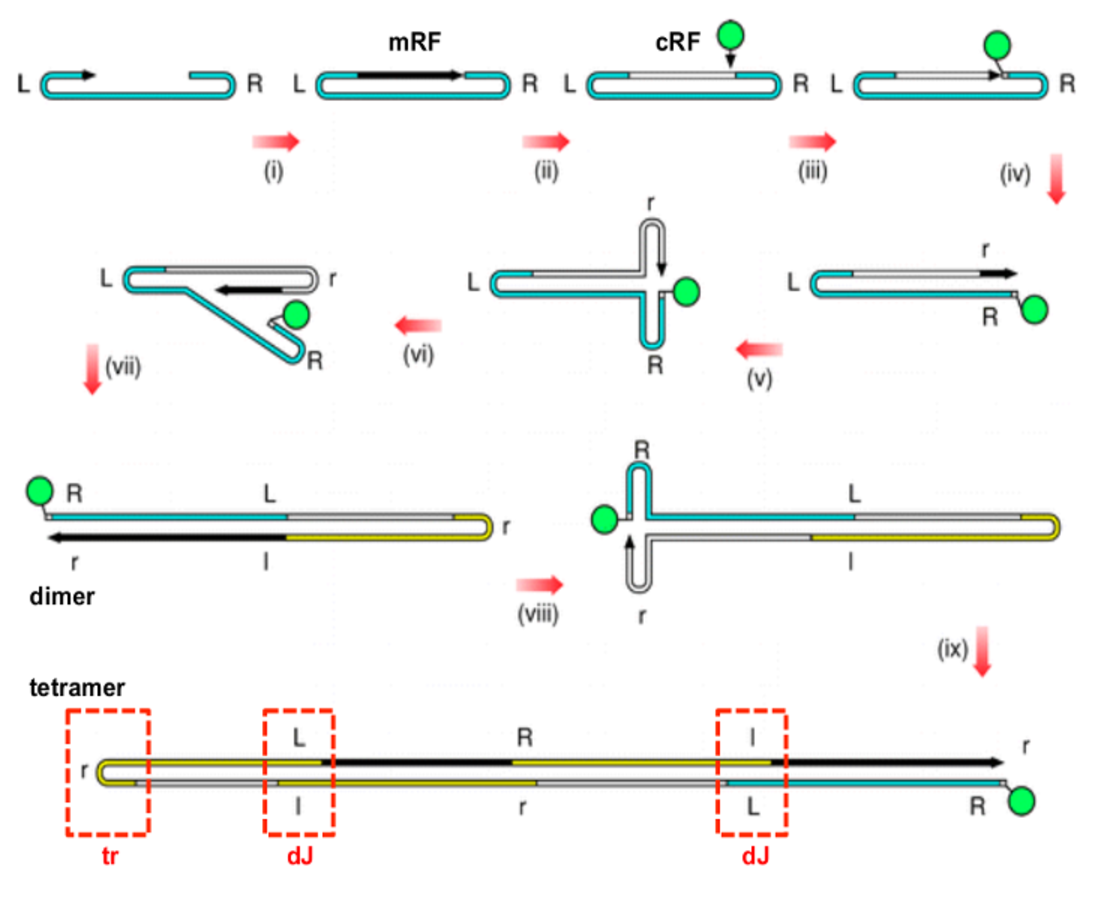
\includegraphics[scale=0.475]{Replication}
  \caption[Rolling hairpin replication (RHR)]
   {Modified rolling hairpin model for MVM DNA replication. The sequence of the parvoviral genome is illustrated by a continuous line, colored blue for the parental genome, yellow for progeny genomes, and black for newly synthesized DNA, the 3’ end of which is capped by an arrowhead. The green sphere represents NS1, which nicks the covalently closed monomer (cRF) and remains attached to its 5’ end. The letters L and R depict the palindromic sequences at each terminus, with their inverted complements represented by l and r, respectively. Red dashed boxes depict the turnaround (tr) form of the right-end and the dimer junction (dJ) form of the left-end palindrome \cite{els}. 
} 
\label{RHR}
\end{figure}

\nomenclature{RHR}{Rolling hairpin replication}
\nomenclature{mRF}{Monomeric replicative form DNA}
\nomenclature{cRF}{Closed replicative form DNA}
\nomenclature{dRF}{Dimeric replicative form DNA}
\nomenclature{PCNA}{Proliferating cell nuclear antigen}
\nomenclature{HSPG}{Heparan sulphate proteoglycan}
\nomenclature{SA}{Sialic acid}
\nomenclature{VLP}{Virus-like particle}
\nomenclature{CLIC}{Clathrin-independent carrier}
\nomenclature{EM}{Electron microscopy}
\nomenclature{PFU}{Plaque-forming unit}
\nomenclature{EGFR}{Epidermal growth factor receptor}
\nomenclature{LamR}{Laminin receptor}
\nomenclature{FGFR1}{Fibroblast growth factor receptor 1}
\nomenclature{HGFR}{Hepatocyte growth factor receptor}
\nomenclature{NHP}{Nonhuman primate}
\nomenclature{PDGFR}{Platelet-derived growth factor}
\nomenclature{hpi}{Hours post-infection}
\nomenclature{EC}{Empty capsid}
\nomenclature{FC}{Full capsid}


\section{Transcription and RNA processing}
\label{Transcription1}
Parvoviruses use a wide variety of alternative RNA processing strategies in order to exploit the strictly limited coding capacity of their small genomes. Alternative splicing of messenger RNA precursors (pre-mRNA) provides a powerful mechanism to generate structurally related but distinct proteins from a single gene, hence contributing to a complex but efficient and compact genome organization \cite{pmid2694943, pmid1335742}. The complex nature of MVM RNA processing of primary transcripts is summarized and simplified in Figure~\ref{Transcription}, p.\pageref{Transcription}. The genome of MVM is transcribed in overlapping transcription units from two promoters located at m.~u. 4 and 38, termed P4 and P38, respectively (see Figure~\ref{Transcription}~A, p.~\pageref{Transcription}) \cite{pmid6828378}. Products of these promoters are three major transcript classes, R1 (4.8 kb) and R2 (3.3 kb), generated from P4, as well as R3 (2.8 kb), generated from P38 \cite{pmid3951017}. All MVM mRNAs are polyadenylated at a single polyadenylation site at the far right-hand end of the genome (see Figure~\ref{Transcription}~B, p.~\pageref{Transcription}) \cite{pmid3660591, pmid3502703}. On the one hand, transcripts R1 and R2 encode the viral NS proteins NS1 and NS2, respectively, utilizing the ORF in the left half of the genome \cite{pmid2939261}. On the other hand, the R3 transcripts encode the overlapping viral capsid proteins VP1 and VP2, utilizing the ORF in the right half of the genome. Additionally, the non-structural SAT protein (see Section~\ref{SAT}, p.~\pageref{SAT}) lies embedded within the capsid genes and likewise, is expressed from the P38 promoter \cite{pmid16189014}. Transcription from the viral early and late promoters is accomplished by the host RNA polymerase~\RM{2} \cite{pmid6828378, polII} and accompanied by various cellular transcription factors \cite{pmid2585609, pmid8009857, pmid2325201, pmid7983715, pmid1942250}. 

All MVM pre-mRNAs contain an overlapping set of downstream small introns in the center of the genome (m.~u. 44-46) that is alternatively spliced using two donor sites (D1 and D2) and two acceptor sites (A1 and A2) \cite{pmid2942705, pmid3783817, pmid2164605, pmid2142555}. In addition to the small downstream intron, P4-generated transcripts also have a large upstream intron, located between m.~u. 10 and 39. Intron splicing events are represented by the thin-lined carets in Figure~\ref{Transcription}~B, p.~\pageref{Transcription}. Excision of the large intron is required to produce the R2 transcripts which encode the three NS2 protein isoforms \cite{pmid6623929, pmid6828378, pmid2942705}. Splicing at this site is critical in determining the steady state levels of NS1 and NS2 (see Section~\ref{NS}, p.~\pageref{NS}) \cite{pmid1825251, pmid2142555}. Since R1 and R2 transcripts have similar stabilities \cite{pmid1825251}, and are transported equally to the cytoplasm \cite{pmid1592259}, the ratio of accumulated levels of R1 transcripts relative to R2 directly depends upon the percentage of P4-generated R2 transcripts which lack the large intron. In this way, MVM manages to maintain the optimal balance between the crucial roles which NS1 and NS2 play in viral replication and cytotoxicity \cite{pmid3296697}. On the contrary, alternative splicing of the small downstream intron from P4-generated pre-mRNAs leads to the production of three isoforms of NS2 \cite{pmid3783817, pmid2142555, pmid2164605} of the one part and the two structural capsid proteins, derived from P38-generated R3 transcripts, of the other part. The joining of donor D1 to acceptor A1 [major, M ($\sim$70~\%)] produces an mRNA which encodes the major capsid protein VP2, or a mRNA encoding NS2\textsuperscript{P} from R3 or R2 transcripts, respectively. Alternatively, joining of D2 to A2 [minor, m ($\sim$25~\%)] generates an mRNA encoding the minor capsid protein VP1, or an mRNA that encodes NS2\textsuperscript{Y} from R3 or R2 transcripts, respectively. Finally, a rare splicing pattern that joins D1 to A2 [rare, r ($\sim$5~\%)] is required for the production of NS2\textsuperscript{L} encoding mRNAs from R2 transcripts \cite{pmid3502703, pmid2942705, pmid3783817, pmid3951017}. The fourth splicing pattern that joins D2 to A1 is not detected \textit{in vivo} \cite{pmid3783817}, presumably because the distance between this sites (60 nts) is too short to enable successful excision of introns in mammalian cells \cite{pmid2943217}. To date, only a few examples of small overlapping introns with two donors and two acceptors have been described in literature \cite{pmid1335742, pmid1824726, pmid1839712}. For MVM, the small central intron, which is excised efficiently from all classes of MVM pre-mRNA transcripts, appears to be the entry of the spliceosome. In addition, it dictates the relative amounts of VP1 and VP2 or of the three isoforms of NS2 produced during infection. Splicing of the large upstream intron occurs subsequent to small intron recognition and splicing. This second processing step is slowed to make sure that the spliced RNA can leave the nucleus to encode NS1. This delay is most likely ensured by the large non-consensus donors and acceptors of the splice site of the large intron \cite{Transcription}. However, the determinants governing the alternative excision of the large and small intron from MVM pre-mRNAs are poorly understood \cite{pmid9499034, pmid10329570, pmid8151756, pmid7666519, pmid7637034, pmid9858560}. Nonetheless, it is known that wild-type patterns of alternative splicing of MVM pre-mRNAs are achieved exclusively by cellular splicing factors without the involvement of auxiliary viral proteins \cite{pmid1592259}. Moreover, it has bee shown that polyadenylation of MVM RNAs precedes splicing of the small intron since unspliced polyadenylated molecules can be detected in the nucleus. In contrast, no detectable accumulation of unspliced MVM RNAs were observed in the cytoplasm of infected cells \cite{pmid3346950}. This does not apply for the large intron which is only spliced in a proportion of the pre-mRNAs prior to its export from the nucleus. Once in the cytoplasm, R1 transcripts are prevented from further splicing to R2 transcripts. The mechanisms that regulate the export of R1 versus its nuclear retention and further splicing to R2 remain elusive \cite{Transcription}. All aforementioned splicing patterns are exemplified in Figure~\ref{Transcription}~B, p.~\pageref{Transcription}. 

Although viral proteins are not participating in the regulation of alternative splicing, they are indispensable for controlling transcription, along with relevant cellular transcription factors and viral \textit{cis}-acting sequences. Interestingly, there is a chronological order to the production of MVM RNA transcripts. It was demonstrated that R1 and R2, the P4-generated pre-mRNAs, precede the P38-generated R3 transcripts during synchronous infection \cite{pmid3346950}. This temporal phasing is the result of NS1-dependent up-regulation of transcription from the P38 promoter \cite{pmid3171551, pmid4020972}. The acidic C-terminal domain of NS1 acts as a classical transcriptional activator that can potentiate P38 transcription approximately 100-fold \cite{pmid1388209}. In this way, the NS proteins, particularly NS1 that is essential for MVM DNA replication (see Section~\ref{Replication}, p.~\pageref{Replication}) are available prior to the structural capsid proteins in order to initiate early events in parvoviral infection and to stimulate the transcription of the VP and SAT genes under the control of the late P38 promoter. An example for viral \textit{cis}-acting sequences that regulate infection can be found in the left-end hairpin sequence, where both transcription and replication factors compete for specific recognition elements distal to the bubble sequence. Binding of cAMP-responsive element (CRE) to this sequence has been shown to contribute to maintaining basal levels of P4 activity and also to the up-regulation of P4 activity in transformed cells \cite{pmid7636996, pmid8627649}. CRE binding overlaps with the distal of the two 5'-ACGT-3' half sites needed to bind PIF (see Figure~\ref{Architecture}~C, p.~\pageref{Architecture}) which is essential for stabilizing NS1 binding to the active left-end origin (\textit{OriL\textsubscript{TC}}) for replication initiation (see Section~\ref{sec: Architecture}, p.~\pageref{sec: Architecture}) \cite{pmid12050365}. In this way, replication and transcription are in competition with each other co-ordinate viral infection.            

       

\begin{figure}[H]
\centering
  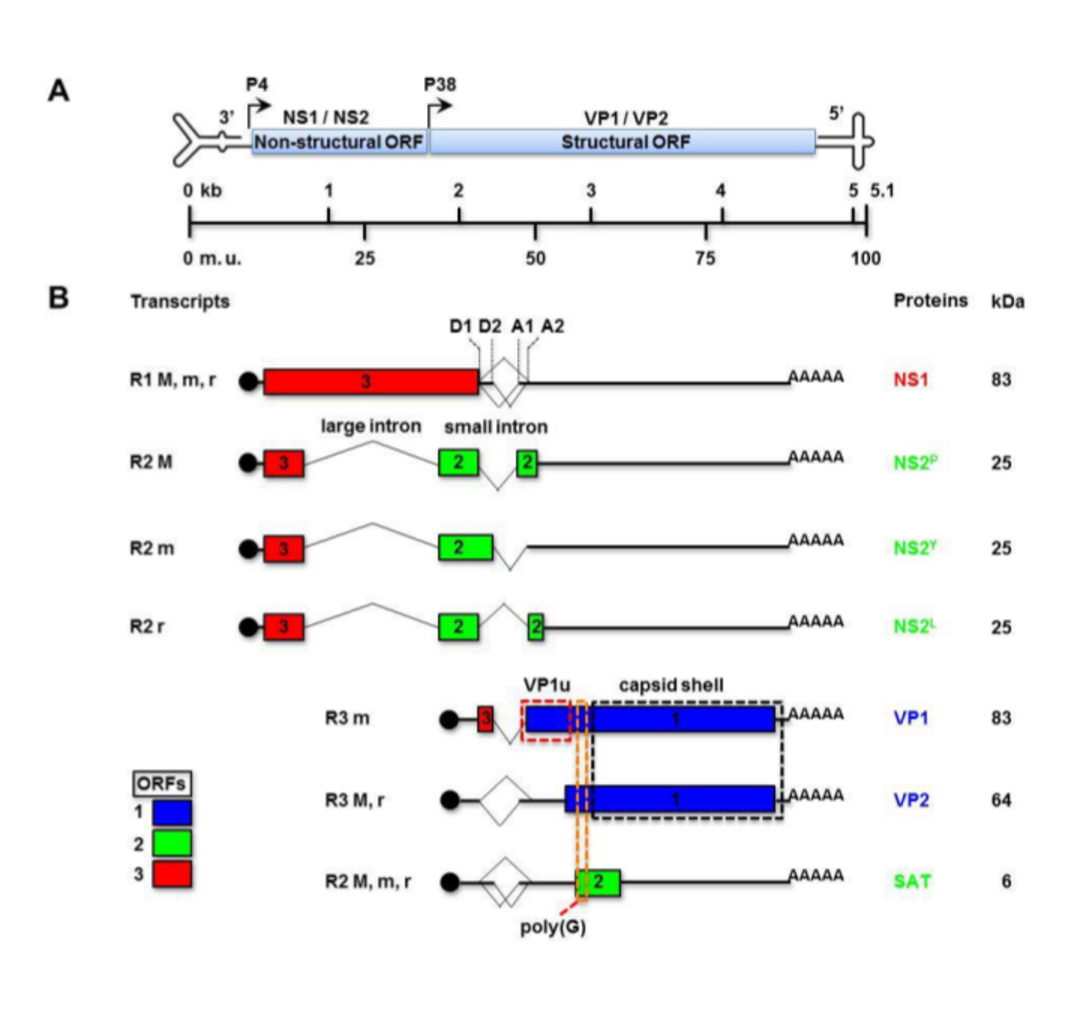
\includegraphics[scale=0.65]{Transcription}
  \caption[Transcription map of MVM]
   {Transcription map of MVM. \textbf{(A)} The single-stranded, negative-sense DNA genome of MVM is illustrated by a single line terminating in dissimilar hairpin telomeres. The two major ORFs are boxed in light blue and the proteins which they encode are indicated above. The two viral promoters, P4 and P38 are shown by rightward arrows. Below, arbitrary m.~u. are diagrammed relative to the 5.1 kb genome. \textbf{(B)} The three major cytoplasmic transcript classes R1, R2, and R3 are displayed. A black sphere indicates the capped 5’ ends and (AAAAA) denotes their polyadenylated tails near the far right-hand end of the genome. ORFs encoding the viral proteins, named on the right, are displayed in different coloring according to their reading phase. Their spliced-out large or small introns are indicated by thin-lined carets. The small intron is excised from each transcript class by the alternative use of three different splicing patterns, denoted M (major), m (minor), and r (rare). Splice donor and acceptor sites for splicing of the small intron are denoted D1, D2 and A1, A2, respectively. On the one hand, alternative splicing of the small intron generates the R3 transcripts encoding VP1 and VP2, the two structural capsid proteins, and the R2 transcripts encoding three C-terminally distinct isoforms of NS2, referred to as NS2\textsuperscript{P}, NS2\textsuperscript{Y}, and NS2\textsuperscript{L}. On the other hand, excision of the large intron is critical in determining the steady state levels of NS1 and NS2 transcripts. The N-terminal protein sequence boxed in red represents VP1u which harbors the PLA\textsubscript{2} motif that is involved in entry functions. Sequences boxed in black, comprising the C-terminal region common to all VP polypeptides, assemble to form the capsid shell. Poly(G), boxed in orange, identifies a short glycine-rich region present in all VPs that can be modeled into X-ray density occupying the fivefold pores in virions. This Figure was adapted from \cite{small}}
\label{Transcription}
\end{figure}       



\nomenclature{pre-mRNA}{messenger RNA precursor}
\nomenclature{mRNA}{messenger RNA}
\nomenclature{m.~u.}{Map unit}
\nomenclature{TfR}{Transferrin receptor}

\section{Assembly}
\label{Assembly}

The assembly of MVM capsids occurs in the nucleus and involves cytoplasmic trimerization of viral structural proteins and subsequent nuclear translocation of those trimers (see Section~\ref{Struc Transloc}, p.~\pageref{Struc Transloc}) \cite{pmid16469332}. The formation of trimers results from extensive intertwinement of the VP polypeptides through extended surface loops which form tight, convoluted intratrimer interactions (see Figure~\ref{Structure1}, p.~\pageref{Structure1}) \cite{pmid15299974, pmid21867712}. These trimers are incompetent for capsid assembly in the cytoplasm. In order to confer nuclear assembly, the trimeric precursors undergo a global conformational rearrangement on top of the 3-fold spike at the center of each trimer \cite{pmid16469332, pmid12552010, pmid17626084}. Nuclear association of trimeric assembly intermediates is mainly mediated by quasi-linear, hydrophobic interactions between trimeric subunits. Polar interactions only marginally contribute to capsid assembly and stability \cite{pmid14981262}.     

Currently, it remains uncertain whether auxiliary nuclear factors are required for the final steps of parvovirus assembly and maturation. There is evidence that the formation of MVM capsids requires both nuclear factors and the major capsid protein VP2. Expressed capsid proteins that were incompetent for nuclear localization, as well as singly expressed nuclear transport competent VP1 proteins in the absence of VP2 proteins, were not able to assemble \cite{pmid12072505, pmid10438891, pmid10729155}. In the case of B19V it was demonstrated that VP1 deletion mutants formed morphologically normal capsids but only a limited extension of VP1 was tolerated. Further lengthening of VP1 versions resulted in less efficient assembly and any assembled particles showed dysmorphic appearance \cite{pmid8207846}. Truncations beyond 30 amino acids at the N-terminus of VP2 prevented assembly because they affected the $\beta$A-strand of the conserved $\beta$-barrel motif which constitutes the core of the capsid shell (see Figure~\ref{Structure1}, p.~\pageref{Structure1}) \cite{pmid7666560}.     


Nuclear assembly occurs regardless whether the host cell is in S-phase. Inhibition of DNA synthesis resulted in a reduction of mature virions. Nonetheless, ECs accumulated in the nucleus of infected cells \cite{pmid559779, assembly}. The viral NS2 protein was reported to play a host-range specific role in MVM capsid assembly. On the one hand, MVM expressing truncated forms of NS2 was able to give rise to progeny virus in transformed human cells, albeit with reduced efficiency. On the other hand, they were unable to assemble in their restrictive murine host cells in spite of properly expressing NS1 and the structural proteins in early stages post-infection. The involvement of NS2 in virus assembly remains elusive but is likely to be indirect, since an appropriate cellular environment can complement the defect \cite{pmid9168889}.        


A better understanding of the mechanisms underlying capsid assembly and disassembly will be fundamental to the development of antiviral drugs. Virus propagation may be prevented by interference with capsid assembly or by promoting or inhibiting capsid disassembly \cite{pmid21762804, pmid21163649}. Further applications include the use of self-assembling viral nanoparticles for biomedical and nanotechnological applications \cite{pmid16521330, pmid16690856}.     


  
\section{DNA Packaging}
\label{Packaging}

Commonly, viruses use two alternative strategies to package their genomes into the capsids. On the one hand, viruses containing circular dsDNA genomes assemble their protein shell around the genome, driven by interactions between protein capsid subunits and nucleic acids and assisted by auxiliary scaffolding proteins \cite{pmid6101085, pmid6305987, pmid1323699}. Moreover, several ssDNA or ssRNA viruses, such as tobacco mosaic virus, F1, and M13 bacteriophage follow the same assembly pathway via association of structural proteins around the genome \cite{pmid11406604}. On the other hand, viruses with double-stranded linear genomes translocate their genetic material into pre-assembled ECs. This process is ATP-dependent and involves auxiliary non-structural packaging enzymes \cite{pmid2679356}. The presence of a large excess of ECs in parvovirus stocks and the fact that recombinant expression of their structural proteins is sufficient for capsid formation \cite{pmid1331503} implies that the viral DNA is not required for capsid assembly. Thus, parvoviruses use the latter mechanism for genome translocation into their pre-formed capsids which accumulate in the cell nucleus (see Section~\ref{Assembly}, p.~\pageref{Assembly}). Significantly, the encapsidation process has been visualized by EM in an \textit{in vitro} assembly and packaging reaction of Lu\RM{3} parvovirus \cite{pmid6221078}.

In the case of MVM, partially or fully packaged capsids were demonstrated to interact with NS1. The NS protein was covalently attached to the 5' termini of unit-length ssDNA genomes. These structures may represent intermediates of the packaging process and NS1, particularly its 3' to 5' helicase activity (see Section~\ref{NS1}, p.\pageref{NS1}) may support genome translocation into the pre-assembled capsid \cite{pmid2527311}. Similar observations were reported for AAV2 capsids which were shown to interact with the homologous \textit{rep} proteins \cite{pmid8553536, pmid8995658}. DNase protection studies in AAV \cite{pmid11406604} and binding experiments between DNA and capsids of autonomous parvoviruses \cite{pmid2145445, pmid8350419} suggest a 3’ to 5’ packaging direction for parvoviruses. According to the directionality of the encapsidation process, the 3’ to 5’ processivity of the virus-encoded helicase, rather than the strand displacement 5' to 3' RHR synthesis, seem to drive the translocation of the genome into pre-formed capsids \cite{pmid11406604}. 

Initiation of the encapsidation process involves viral \textit{cis}-acting elements. The ITRs of AAV contain a packaging signal which is both required and sufficient for genome encapsidation \cite{pmid2547998}. So far, a direct, specific interaction of AAV ITRs with capsids has not been demonstrated \cite{pmid8627687, pmid9060669}. In contrast, specific binding of the 3' terminal repeat of MVM to VP1 \cite{pmid1870193} and to particles composed only of VP2 \cite{pmid8350419} have been reported. However, interaction with VP1 is not essential for genome translocation since VP1 is dispensable for MVM assembly and packaging \cite{pmid8416366}.      

Cross-packaging of Lu\RM{3}-derived vector genomes into capsids of MVM reinforced the observation that strand selection for packaging occurs due to varying efficiency of excision from replicated genomes of one strand polarity \textit{versus} the other rather than differences in packaging preference \cite{pmid15866075}. This phenomenon is further elucidated in Section~\ref{Resolution}, p.~\pageref{Resolution}.   
\label{Packaging1} 

\section{Nuclear Export}
\label{Export}
Besides having the possibility to passively egress the host cell by NS1-induced cellular lysis, the latest data of several research groups propose an active, pre-lytic egress for MVM (see Section~\ref{Egress}, p.~\pageref{Egress}) \cite{pmid24068925, pmid18704167, pmid15367635}. In order to actively egress the host cell, progeny particles of karyophilic viruses need to cross considerable cellular barriers. Apart from the plasma membrane, the nuclear envelope constitutes a second barrier to MVM. Although the mechanism for nuclear export and subsequent release of MVM virions remains unknown, several important viral and cellular effectors involved in PV egress have been identified and characterized. 

MVM is supposed to be exported from the host’s nucleus by a Crm1 dependent mechanism. A stable interaction between NS2 and Crm1 has been documented \cite{pmid10438867, pmid10527855}. Classical nuclear export signals (NES) exhibit low affinity for Crm1 in order to prevent the formation of the Crm1/cargo complex in the cytoplasm where RanGTP is absent \cite{pmid10449743}. Surprisingly, the NES of NS2 belongs to the supraphysiological NES which tightly bind to Crm1 regardless of the presence of RanGTP. Therefore, NS2 competitively inhibits Crm1 function by sequestering endogenous nuclear export receptors. MVM mutant genomic clones generating NS2 proteins harboring either regular NES, or substitutions which abrogated Crm1 interaction were shown to be compromised in viral nuclear export and productive infection \cite{pmid18385513}. As expected, NS2-Crm1-mutants showed nuclear accumulation of export deficient NS2 in transfected cells. Surprisingly, the nuclear retention of mutant NS2 proteins came along with a substantial accumulation of progeny virions in the nucleus of infected cells, suggesting a NS2-dependent export of progeny virions. Additionally, an indirect involvement of NS2 in viral egress was demonstrated using the closely related H1-PV. For this virus, an in-frame deletion of 38 amino acids within the common coding sequence of NS1 and NS2 was demonstrated to beneficially influence infectivity \textit{in vitro}, indicated by a lower particle-to-infectivity (P/I) ratio and a larger plaque phenotype. The increase in infectivity which resulted from an accelerated egress of the mutant progeny virions, positively affected tumor growth suppression \textit{in vivo} \cite{pmid22553326}. However, approaches to demonstrate a direct interaction between NS2 and the viral capsid and/or individual structural proteins \textit{in vitro} have not yet been successful despite extensive attempts. Such interactions might be very weak and highly dynamic, thus it is difficult to demonstrate them.  


The differences in nuclear export observed during productive MVM infection in either permissive human cells or restrictive murine cells may be due to cell-type-specific use of alternative strategies for nuclear export. They became particularly apparent when the different cell types were treated with the anti-fungal antibiotic leptomycin B (LMB) to inhibit Crm1-dependent nuclear export \cite{pmid9683540}. LMB treatment of susceptible murine cells resulted in a significant but not complete inhibition of nuclear export of MVM progeny virions. In contrast, even high doses of LMB did not inhibit nuclear export of MVM in transformed human cells, indicating that Crm1 is not required for the nuclear export of MVM in these cells \cite{pmid15367635}. The observed differences may result from a cell-type dependent phosphorylation status of MVM. Generally, MVM capsids derived from permissive human cells displayed prominent phosphorylation compared to the decent phosphorylation status of capsids isolated from restrictive murine fibroblasts \cite{pmid11069983}. Significantly, the three distal serine residues at position 2, 6, and 10 of the unordered N-VP2 terminus showed high phosphorylation levels in permissive cells. Site-directed mutagenesis studies discovered an important role of these phosphorylations in the Crm1-independent nuclear export of MVM in permissive human cells. When the N-terminal phosphorylations were diminished, progeny virions were predominantly retained in the nucleus and the corresponding mutants displayed a small plaque phenotype, indicating the importance of those phosphorylations in viral spread \cite{pmid15367635}. 

\nomenclature{LMB}{Leptomycin B}  

\section{Egress}
\label{Egress}
MVM transport from the nucleus to the cell periphery is associated with the degradation of actin fibers and the formation of “actin-patches”. These alterations to the filamentous network were attributed to a virus-induced imbalance between the actin polymerization factor neural Wiskott-Aldrich syndrome protein and gelsolin, a member of the actin-severing protein family \cite{pmid15582663}. Indeed, the MVM titer in the culture medium following MVM infection drastically declined when gelsolin function was diminished. During MVM infection, gelsolin activity is regulated by the CK\RM{2}$\alpha$/NS1 complex which was demonstrated to be capable of phosphorylating gelsolin. Consequentially, inhibition of CK\RM{2}$\alpha$ correlated with prolonged persistence of actin fibers and delayed formation of the characteristic “actin patches” \cite{pmid18704167, pmid16641266}. A great deal of experimental data would point to an active, vesicle-associated, gelsolin-dependent export of MVM. Progeny virions were shown to co-localize with exocytic, endosomal, and lysosomal markers in immunofluorescent experiments \cite{pmid18704167, pmid17287256}. Cell fractionation experiments confirmed this observation by demonstrating a co-migration of viral particles with cytosolic vesicles rather than free, vesicle-independent localization in the soluble cytosolic fraction. Furthermore, dynamin was found to accumulate in the perinuclear region where it co-localized with \textit{de novo} synthesized MVM capsids. A co-operative cross-talk between actin- and microtubule dependent transport \cite{pmid15040446, pmid12383793, pmid17998399} might be involved in MVM transport from the nucleus to the cell periphery, resulting in the destruction of actin filaments and the stabilization of microtubules \cite{pmid18704167}.  

The secretory pathway has been proposed as the route for active egress of MVM. Progeny virions would become engulfed by COPII-vesicle formation in the perinuclear ER where they accumulated with dynamin. Accordingly, a dramatic retention of virions in the perinuclear area and inhibition of virion release into the medium was observed in cells lacking functional effectors of the secretory pathway \cite{pmid24068925}. However, no significant co-localization between MVM progeny virions and representative markers of the recycling pathway or the Trans Golgi Network (TGN) were evident \cite{pmid24068925}. Radixin and moesin were shown to play a role in virus maturation and spreading capacity, as judged by their impact on MVM plaque morphology \cite{pmid19321616}. Indeed, dominant negative mutants failed in wrapping progeny virions into transport vesicles, resulting in a marked reduction of egressed virions in the culture medium. As a consequence, corresponding markers for alternative export routes, e.g. direct transport from the TGN to the PM or through recycling endosomes, exhibited increased co-localization with progeny virions. Finally, active egress promotes cellular lysis as demonstrated by the prolonged viability of cells wherein vesicular transport was either inhibited or by-passed the Golgi apparatus. In addition, the involvement of progeny particles in cytolysis was demonstrated by the prolonged survival of murine cells transduced with a viral vector deficient for the production of progeny virion particles \cite{pmid24068925}.  
\label{Egress1}



  

\nomenclature{TGN}{Trans Golgi network}
\nomenclature{ER}{Endoplasmic reticulum}


 
%\input{./Chapters/Chapter8} 
%\input{./Chapters/Chapter9} 


\part{Methods}
% Chapter 2

\chapter{Methods} % Main chapter title

\label{ChapterX} % For referencing the chapter elsewhere, use \ref{Chapter2} 

% \lhead{Chapter 2. \emph{Methods}} % This is for the header on each page - perhaps a shortened title

%----------------------------------------------------------------------------------------

\section{Cell Cultures}
A9 ouab\textsuperscript{r}l1 cells, a derivative from the original HGPRT\textsuperscript{-} L-cell line A9 represent a clone resistant to 10\textsuperscript{-3} M ouabain after nitrosoguanidine mutagenesis \cite{pmid6602222, pmid14213660}.
NB324K cells are a clone of SV40-transformed \nomenclature{SV40}{Simian vacuolating virus 40 or Simian virus 40} human newborn kidney cells \cite{pmid13911591}. The SV40 large T antigen was detected by immunofluorescent \nomenclature{IF}{Immunofluorescence microscopy} staining with monoclonal antibodies (mAb) \cite{pmid6169844}. \nomenclature{mAb}{Monoclonal antibody} However, NB324K cells do not produce infectious SV40 spontaneously.
Both cell lines, A9 mouse fibroblasts and NB324K cells, were routinely propagated under a minimal number of passages in Dulbecco's Modified Eagle Medium (DMEM) (see Table~\ref{Media}, p.~\pageref{Media}) supplemented with 5~\% of heat inactivated fetal calf serum (FCS) at 37~\textcelsius~in 5~\% CO\textsubscript{2} atmosphere.

\nomenclature{FCS}{Fetal calf serum} 
\nomenclature{DMEM}{Dulbecco modified Eagle's medium}

\subsection{Freezing and thawing of cells}
Before use, the A9 mouse fibroblasts or NB324K cells were thawed at 37 \textcelsius~ and cultured in 5 mL of pre-warmed DMEM (see Table~\ref{Media}, p.~\pageref{Media}) supplemented with 5~\% FCS. The medium was replaced every 3 to 4 days. 
In order to freeze the cells for long storage in liquid nitrogen they were passed the day before in DMEM containing 10~\% FCS, to ensure exponential growth. Subsequently, 7.5~\% DMSO was added and the cells were frozen slowly at -70 \textcelsius~ over night before transfer to liquid nitrogen.

%----------------------------------------------------------------------------------------

\section{Virus Stocks}
\label{Virus Stocks}
Stocks of MVM without detectable levels of VP3 were propagated on A9 mouse fibroblast monolayers. As soon as the cytopathic effect was complete (7-8 days post-infection), the supernatant (SN) was collected and pre-cleared from cell debris by low-speed centrifugation. Thereby, intracellular VP3 rich capsids were discarded. In order to remove low-molecular contaminants, virus containing SN was pelleted through 20~\% sucrose cushion in PBS by ultra-centrifugation. Virus titers were determined by quantitative PCR (qPCR) (see Section~\ref{qPCR}, p.\pageref{qPCR}) as DNA-packaged particles per microliter.   

\nomenclature{SN}{Supernatant}
\nomenclature{qPCR}{Quantitative PCR} 
\nomenclature{PCR}{Polymerase chain reaction}

\subsection{Separation of empty and full capsids}
\label{CsCl}
Sucrose purified capsids were prepared as previously described in Section~\ref{Virus Stocks}, p.~\pageref{Virus Stocks}. The virus pellet was resuspended in 10 mL PBS. Caesium chloride was added to a density of 1.38 g/mL adjusted by refractometry ($\eta$=1.371) at 4~\textcelsius. The gradient was centrifuged to equilibrium for 24 h at \np{41000} rpm and 4~\textcelsius~in a Beckman SW-41 Ti swinging bucket rotor. Gradients were fractionated and tested for intact capsids by dot blot analysis using B7 mAb (see Table~\ref{Primary antibodies}, p.~\pageref{Primary antibodies}). CsCl was depleted from the corresponding fractions by size-exclusion chromatography through PD-10 desalting columns (GE Healthcare) and the capsids were concentrated in Amicon\textsuperscript{\textregistered} centrifugal filter devices (Merck Millipore) when required.          
   
   


\section{Freezing bacteria stocks in glycerol}
Bacteria were frozen in dry ice. A volume of 700 $\mu$L of the bacteria culture that was grown over night in LB-medium (see Table~\ref{Media}, p.~\pageref{Media}) was mixed with 300 $\mu$L of 50~\% glycerol in a cryotube. In order to mix well the glycerol the cryotube was vortexed intensively. Following snap-freeze in dry ice the bacteria were stored at -70 \textcelsius.


\section{Fast protein liquid chromatography (FPLC)}
\label{ÄKTA}

\begin{figure}[H]
\centering
  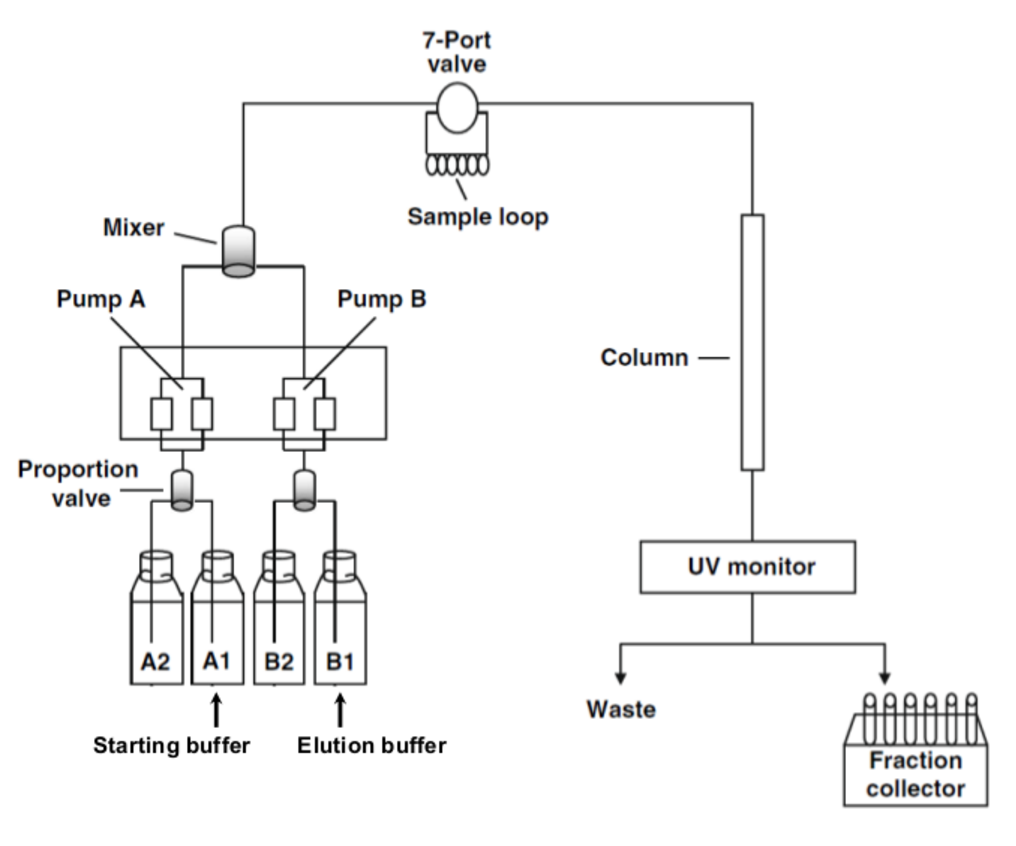
\includegraphics[scale=0.7]{FPLC}
  \caption[Schematic outline of the ÄKTA chromatography system]
   {Schematic outline of the ÄKTApurifier 10/100 UPC-900 chromatography system. This figure was adapted from \cite{pmid20978981}.} 
\label{FPLC}
\end{figure}


\subsection{Anion-exchange chromatography (AEX)}
\label{AEX}
A Mono Q\textsuperscript{\texttrademark} HR 5/5 (Pharmacia) column (5 x 50 mm) was used to analyse virus samples. The Mono Q column was connected to the ÄKTApurifier 10/100 UPC-900 chromatography system (GE Healthcare) that was operated by the unicorn control software (GE Healthcare). The Mono Q\textsuperscript{\texttrademark} column was equilibrated with five column volumes (CV) starting buffer (see Table~\ref{AEX buffers}, p.~\pageref{AEX buffers}). Samples (1 mL) containing at least 10\textsuperscript{10} DNA-containing virus particles in sample buffer (see Table~\ref{AEX buffers}, p.~\pageref{AEX buffers}) were applied to the Mono Q\textsuperscript{\texttrademark} column through a 2 mL injection loop. Following sample application the loop and the column were rinsed with six CV starting buffer. In order to elute the bound proteins, a linear salt gradient (0-2 M NaCl) was applied by gradually increasing the concentration of the elution buffer (see Table~\ref{AEX buffers}, p.~\pageref{AEX buffers}). The total elution volume of 24 CV was split into fractions of 185 $\mu$L which were collected in 96-well plates. The flow rate was kept constant at 1.5 mL/min and the salt concentration was monitored by measuring its electrical conductivity. Viral genomes in each fraction were quantified by qPCR (see Section~\ref{qPCR}, p.~\pageref{qPCR}).  

Increased back-pressure, color change at the top of the column, decreased sample recoveries, or loss of resolution indicate that the column matrix requires regeneration. In order to circumvent such problems, the column was washed every tenth run. To eluate contaminants that stick tightly to the column the following harsh washing steps, summarized in Table~\ref{Washing}, were applied to the reversed (bottom to top) Mono Q\textsuperscript{\texttrademark} column. 

\begin{table}[H]
\begin{center}
\begin{tabular}{c l r r}
\textbf{Step} & \textbf{Reagent} & \textbf{Concentration} & \textbf{Volume} \\
\hline
\\
1 & NaCl & 2 M & 500 $\mu$L \\ 
2 & NaOH & 2 M & 500 $\mu$L \\
3 & Acetic acid & 75 \% & 500 $\mu$L \\
4 & Starting buffer (see Table~\ref{AEX buffers}, p.~\pageref{AEX buffers}) & - & 10 mL \\
\\ 
\end{tabular}
\caption[Cleaning of the Mono Q\textsuperscript{\texttrademark} HR 5/5 AEX column]{Steps 1-4 were performed to wash the Mono Q\textsuperscript{\texttrademark} HR 5/5 AEX column. The column was rinsed with 2 CV water in between each purification step.}
\label{Washing}
\end{center}
\end{table}
All runs were performed at 6 \textcelsius. Buffers were filtered and degassed before application to the Mono Q\textsuperscript{\texttrademark} column.

\nomenclature{CV}{Column volume}


%\subsection{Chromatofocusing (CF)}
%\label{CF}
%
%A Mono P\textsuperscript{\texttrademark} 5/200 GL (GE Healthcare) column (5 x 200 mm) was used to determine the isoelectric points (pI) of virus samples.  The column was connected to the ÄKTApurifier 10/100 UPC-900 chromatography system (GE Healthcare) that was operated by the unicorn control software (GE Healthcare). The Mono P\textsuperscript{\texttrademark} column was equilibrated with two CV of buffer A (see Table~\ref{CF buffers}, p.~\pageref{CF buffers}). Samples (500 uL) containing 10\textsuperscript{10} DNA-containing virus particles in buffer A (see Table~\ref{CF buffers}, p.~\pageref{CF buffers}) were applied to the Mono P\textsuperscript{\texttrademark} column through a 1 mL injection loop. Following sample application, the loop and the column were rinsed with 10 mL buffer A (see Table~\ref{CF buffers}, p.~\pageref{CF buffers}). Bound viruses were eluted by applying buffer B (see Table~\ref{CF buffers}, p.~\pageref{CF buffers}) to the column. Buffer B contains the acidic ampholyte solution, thus gradually lowering the pH within the column. The total elution volume of 7 CV was split into fractions of 250 $\mu$L which were collected in 96-well plates. The flow rate was constantly kept at 0.5 mL/min and the pH was monitored. Viral genomes in each fraction were quantified by qPCR (see Section~\ref{qPCR}, p.~\pageref{qPCR}).      

%All runs were performed at 6 \textcelsius. Buffers were filtered and degassed before application to the Mono P%\textsuperscript{\texttrademark} column.

%\nomenclature{pI}{Isoelectric point}

\section{Quantitative PCR (qPCR)}
\label{qPCR}
Amplification of MVM DNA and real-time detection of PCR products were performed by using CFX96 technology (BioRad) with iTaq\textsuperscript{\texttrademark} Universal SYBR\textsuperscript{\textregistered} Green Supermix (see Table~\ref{Kits}, p.~\pageref{Kits}). PCR was carried out by using the hot-start iTaq\textsuperscript{\texttrademark} DNA polymerase (BioRad) following the manufacturer’s guidelines. Viral DNA was isolated using the DNeasy blood and tissue kit (see Table~\ref{Kits}, p.~\pageref{Kits}). Elution of the purified vDNA was carried out using 100 $\mu$L elution buffer. As templates 2 $\mu$L of the isolated viral DNA were used for the PCR reaction as outlined in Table~\ref{Master mix}.

\begin{table}[H]
\begin{center}
\begin{tabular}{l r r}
\textbf{Component} & \textbf{Amount} & \textbf{Final concentration}\\
\hline
dH\textsubscript{2}O, PCR grade & 6 $\mu$L & -\\
Forward primer (CR3), 10 pM & 1 $\mu$L & 0.5 pM\\
Reverse primer (CR4), 10 pM & 1 $\mu$L & 0.5 pM\\
2x IQ\textsuperscript{\texttrademark} SYBR\textsuperscript{\textregistered} Green Supermix & 10 $\mu$L & 1$\times$\\
\hline
\textbf{Total volume} & \textbf{18 $\boldsymbol{\mu}$L} & \\
\end{tabular}
\end{center}
\caption[Master mix for quantitative PCR]{Master mix for quantitative PCR. In order to minimize pipetting errors a master mix was prepared. Following preparation the master mix was distributed across the 96 well plates. The master mix contains all the ingredients which are required for the DNA amplification except the initial DNA template that differs among the samples.}
\label{Master mix}
\end{table} 

To ensure accurate quantification, the 96-well plates containing master mix and template DNA were shortly spun and transferred into the BioRad CFX96 unit. The PCR program used for quantification of viral DNA is detailed in Table~\ref{PCR conditions}.

\begin{table}[H]
\begin{center}
\begin{tabular}{r l r r}
\textbf{Cycles} & \textbf{Step} & \textbf{Temperature} & \textbf{Time}\\
\hline
\par\smallskip
1x & Initial denaturation & 95 \textcelsius & 300 s\\
40x & Denaturation & 95 \textcelsius & 15 s \\
 & Annealing & 61 \textcelsius & 15 s \\
\par\smallskip 
 & Extension & 72 \textcelsius & 15 s \\
1x & Final denaturation & 95 \textcelsius & 60 s \\
1x & Melting curve & 65 \textcelsius~up to 95 \textcelsius & 0.1 \textcelsius/s \\
\end{tabular} 
\end{center} 
\caption[PCR conditions]
   {PCR conditions for the amplification and real-time detection of MVM DNA.}
\label{PCR conditions}
\end{table}

To provide standards for sample quantification, serially diluted plasmids containing the entire MVM genomic DNA were used.
For cell number variations that may exist between the samples, the number of applied cells per PCR reaction needed to be quantified for normalization as well. For this purpose quantification of cellular $\beta$-actin gene was performed. After normalization, direct comparison of the results is possible. $\beta$-actin quantification was carried out with the same PCR conditions outlined in Table~\ref{PCR conditions}, p.~\pageref{PCR conditions} with the annealing temperature (60~\textcelsius) as the only exception.

In Table~\ref{Primers} all primers are listed which were used for MVM genome or $\beta$-actin gene quantification. 
\begin{table}[H]
\begin{center}
\begin{tabular}{l l}
\textbf{Primer} & \textbf{Sequence}\\
\hline
CR3 & 5'-GACGCACAGAAAGAGAGTAACCAA-3'\\
CR4 & 5'-CCAACCATCTGCTCCAGTAAACAT-3'\\
Mouse $\beta$-actin forward & 5'-TGGCACCACACCTTCTACAATGA-3' \\
Mouse $\beta$-actin reverse & 5'-CCGCTCGTTGCCAATAGTGA-3' \\
Human $\beta$-actin forward & 5'-TGCTGTCCCTGTATGCCTCTG-3' \\
Human $\beta$-actin reverse & 5'-AATGCCTGGGTACATGGTGGT-3' \\
\end{tabular} 
\end{center} 
\caption[Primers]{Different primers that were used for qPCR.}
\label{Primers}
\end{table}


\section{Virus infection} 

A9 or NB324K cells (10\textsuperscript{5} for qPCR, IF, and Western blotting (WB) or 3~$\times$~10\textsuperscript{6} for AEX) were infected with MVM (\np{5000} DNA-containing particles per cell, corresponding to approximately 10 PFU/cell \cite{pmid4673484}) for 1 h at 4~\textcelsius~for binding. Unbound virus was removed by washings and the cells were incubated at 37~\textcelsius~to initiate infection. At progressive times post-internalization total cellular DNA was extracted for qPCR analysis (see Section~\ref{qPCR}, p.~\pageref{qPCR}) or cells were fractionated (see Section~\ref{Fractionation}, p.~\pageref{Fractionation}) and subjected to AEX (see Section~\ref{AEX}, p.~\pageref{AEX}).    



\section{Transfection}
NB324K cells at a confluence of 70 \% were trypsinized and resuspended in 10 mL of DMEM (see Table~\ref{Media}, p.~\pageref{Media}) supplemented with 10 \% FCS. A total amount of 10\textsuperscript{6} cells were used for transfection with the AMAXA\textsuperscript{\texttrademark} nucleofector\textsuperscript{\texttrademark}~\RM{2} device following the manufacturer’s instructions. Transfection was carried out with 5 $\mu$g of the infectious clone of MVM (see Section~\ref{IC}, p.~\pageref{IC}, \cite{pmid6345805}) using the V-001 program. As a transfection reagent, AMAXA\textsuperscript{\textregistered} Cell Line Nucleofector\textsuperscript{\textregistered} Kit V (see Table~\ref{Kits}, p.~\pageref{Kits}) was used. Following transfection the weakened cells were maintained in 1.5 mL of pre-warmed culture medium and after 6 h, the culture medium was replaced with an equal amount of pre-warmed culture medium. The cells were further incubated for the required times.
        

\section{Cell fractionation}
\label{Fractionation}
\subsection{Nuclei isolation}
Isolation of A9 and NB324K nuclei was performed by using the Nuclei EZ Prep Nuclei Isolation Kit (see Table~\ref{Kits}, p.~\pageref{Kits}) following the manufacturer’s instructions. In order to obtain highly pure nuclear fractions, the isolated nuclei were pelleted through a sucrose gradient by low speed centrifugation at 500 g for 10 min. Extracted nuclei were lysed in nuclei lysis buffer (see Table~\ref{General buffers}, p.~\pageref{General buffers}) at 4~\textcelsius~for 30 min. Following vortexing thoroughly the nuclear lysate was passed through a 27 G needle 10 times. Debris was removed by centrifugation at \np{10000} rpm for 10 min at 4~\textcelsius.      

\subsection{Extraction of the cytoplasm}
Cytoplasmic fractions were extracted in cell lysis buffer (see Table~\ref{General buffers}, p.~\pageref{General buffers}) at 4~\textcelsius~for 30 min. Following vortexing thoroughly, intact nuclei and cell debris was removed by centrifugation at \np{10000} rpm for 10 min at 4~\textcelsius. 




\section{Immunoprecipitation (IP)}
\textit{In vitro} treated viruses or viruses from cell extracts were transferred to LoBind tubes that were pre-blocked with PBS containing 1~\% bovine serum albumin (PBSA 1~\%). The volume was adjusted to 200 $\mu$L with PBSA 1~\%. The antibody was added in excess and incubated with the viral capsids for 1 h at 4 \textcelsius~ on a rotary shaker. Subsequently, 20 $\mu$L protein G-agarose beads were added. Following overnight incubation at 4 \textcelsius~ and centrifugation at \np{2500} rpm for 5 min the supernatant was discarded. The beads were washed 4 times with PBSA 1~\%. To remove the BSA an additional wash step was carried out with PBS. Finally, the beads were frozen at -20 \textcelsius~ until further use or immediately processed. 

\nomenclature{IP}{Immunoprecipitation}

\section{Dot Blot}
Viruses (10\textsuperscript{8} in 2 $\mu$L) were spotted on a nitrocellulose membrane. The membrane was blocked for 20 min with TBST containing 5~\% milk. The primary antibody was diluted in TBST supplemented with 1~\% milk and incubated for 30 min at room temperature. Unbound antibody was removed by washing the membrane 3 times for 5 min with TBST containing 1~\% milk. The horseradish peroxidase (HRP)-coupled secondary antibody was diluted 1:\np{20000} in TBST supplemented with 1~\% milk and added to the membrane for 30 min. Excess secondary antibody was removed by the same procedure as aforementioned for the primary antibody. The membrane was developed by exposure to photo films.    

\nomenclature{HRP}{Horseradish peroxidase}

\section{SDS-PAGE and Western blotting (WB)}

Immunoprecipitated capsids were dissolved in 20 $\mu$L 1$\times$ protein loading buffer (see Table~\ref{Western blot}, p.~\pageref{Western blot}) containing 2~\% SDS and 10~\% glycerol. The samples were boiled at 96 \textcelsius~ for 8 min. Viral proteins were separated through a NuPAGE\textsuperscript{\textregistered} 10~\% Bis-Tris Gel (Invitrogen). The XCell Sure Lock\textsuperscript{\texttrademark} Electrophoresis Cell (Invitrogen) was used to separate the proteins. The gel was first run at 30 V for 10 min to stack the proteins. In this way, sharper bands could be achieved. Separation of the different proteins was accomplished at 200 V. Following separation, the proteins were blotted on a methanol activated, porous, 0.2 $\mu$m polyvinylidene fluoride (PVDF) Immobilon\textsuperscript{\textregistered} Transfer Membrane (EMD Millipore). Blotting was carried out at 30 V for 1 h 10 min using XCell II\textsuperscript{\texttrademark} Blot Module (Invitrogen). 
The membrane was blocked in TBS-T buffer (see Table~\ref{Western blot}, p.~\pageref{Western blot}) supplemented with 5~\% milk overnight at 4 \textcelsius. Subsequently, the membrane was probed with a polyclonal rabbit antibody against linear MVM-VP epitopes (see Table~\ref{Primary antibodies}, p.~\pageref{Primary antibodies}) that was diluted 1:\np{2000} in 3 mL TBS-T containing 1~\% milk. The first antibody was incubated for 1 h at room temperature. The PVDF membrane was washed in TBS-T for a total 90 min with many buffer replacements. Subsequently, the horseradish peroxidise conjugated secondary antibody (goat $\alpha$-rabbit-HRP, (see Table~\ref{Secondary antibodies}, p.~\pageref{Secondary antibodies}) was added for 1 h at room temperature. This secondary goat anti-rabbit antibody was diluted 1:\np{20000} in TBS-T supplemented with 1~\% milk. To deplete remaining antibodies, the membrane was washed in the same way as described above except for a final wash step with TBS (see Table~\ref{Western blot}, p.~\pageref{Western blot}). VP1, VP2, and possibly VP3 were visualized by a chemiluminescence system (SuperSignal\textsuperscript{\textregistered} West Femto Maximum Sensitivity Substrate, see Table~\ref{Kits}, p.~\pageref{Kits}) following the manufacturer’s instructions. After this treatment, the PVDF membrane was exposed to a film (Amersham Hyperfilm\textsuperscript{\texttrademark} ECL, see Table~\ref{Kits}, p.~\pageref{Kits}). Finally, the film was developed using Anatomix Developer Replenisher Solution and Fixer and Replenisher Solution (see Table~\ref{Kits}, p.~\pageref{Kits}).

\nomenclature{WB}{Western blotting}

\section{Enzymatic reactions}
 
All enzymatic reactions were performed with 10\textsuperscript{8} virus particles in a reaction volume of 50 $\mu$L. Viruses were incubated in PBS for 1.5 h at 37~\textcelsius~with 0.5 mg/mL chymotrypsin (see Table~\ref{Enzymes}, p.~\pageref{Enzymes}). The reaction was blocked by adding 100 $\mu$M chymostatin (see Table~\ref{Chemicals}, p.~\pageref{Chemicals}). 

Phosphatase lambda treatment (\np{2000} Units, see Table~\ref{Enzymes}, p.~\pageref{Enzymes}) was performed in 50 mM Tris-HCl, 100 mM NaCl, 2 mM MnCl\textsubscript{2}, 5 mM DTT, pH 7.8 for 3 h at 37~\textcelsius~in PBSA 1 \% pre-blocked Protein LoBind eppendorf tubes. Phosphatase lambda was inactivated by supplementing the enzymatic reaction with 1 mM Na\textsubscript{3}VO\textsubscript{4} and 1 mM NaF. 

Free DNA was digested using 50 Units DNase~\RM{1} (see Table~\ref{Enzymes}, p.~\pageref{Enzymes}) in 1$\times$ incubation buffer according to the manufacturer’s protocol. DNase~\RM{1} was inhibited by incubation at 75~\textcelsius~for 15 min. 

Negative controls were incubated in the same buffers for the same time.




%----------------------------------------------------------------------------------------





\part{Publication}
\renewcommand{\cftdot}{}
% ChapterPub1
\label{ChapterPub1}

%\lhead{Chapter 2. \emph{Methods}} % This is for the header on each page - perhaps a shortened title

%\pagestyle{empty}

%\setcounter{chapter}{0}
\chapter{Manuscript}
%\addcontentsline{toc}{chapter}{Wolfisberg \textit{et al.}, Journal of Virology, Submitted November 2015}  
\begin{center}
\addtocontents{toc}{\cftpagenumbersoff{chapter}}
\vspace{5.5cm}

\LARGE{\textbf{Late maturation steps in the nucleus preceding pre-lytic active egress of
progeny parvovirus.}}

\vspace{3cm}

Raphael Wolfisberg, Christoph Kempf and Carlos Ros
\end{center}


\phantomsection\addcontentsline{toc}{section}{Late Maturation Steps in the Nucleus Preceding Pre-Lytic Active Egress of Progeny Parvovirus.}



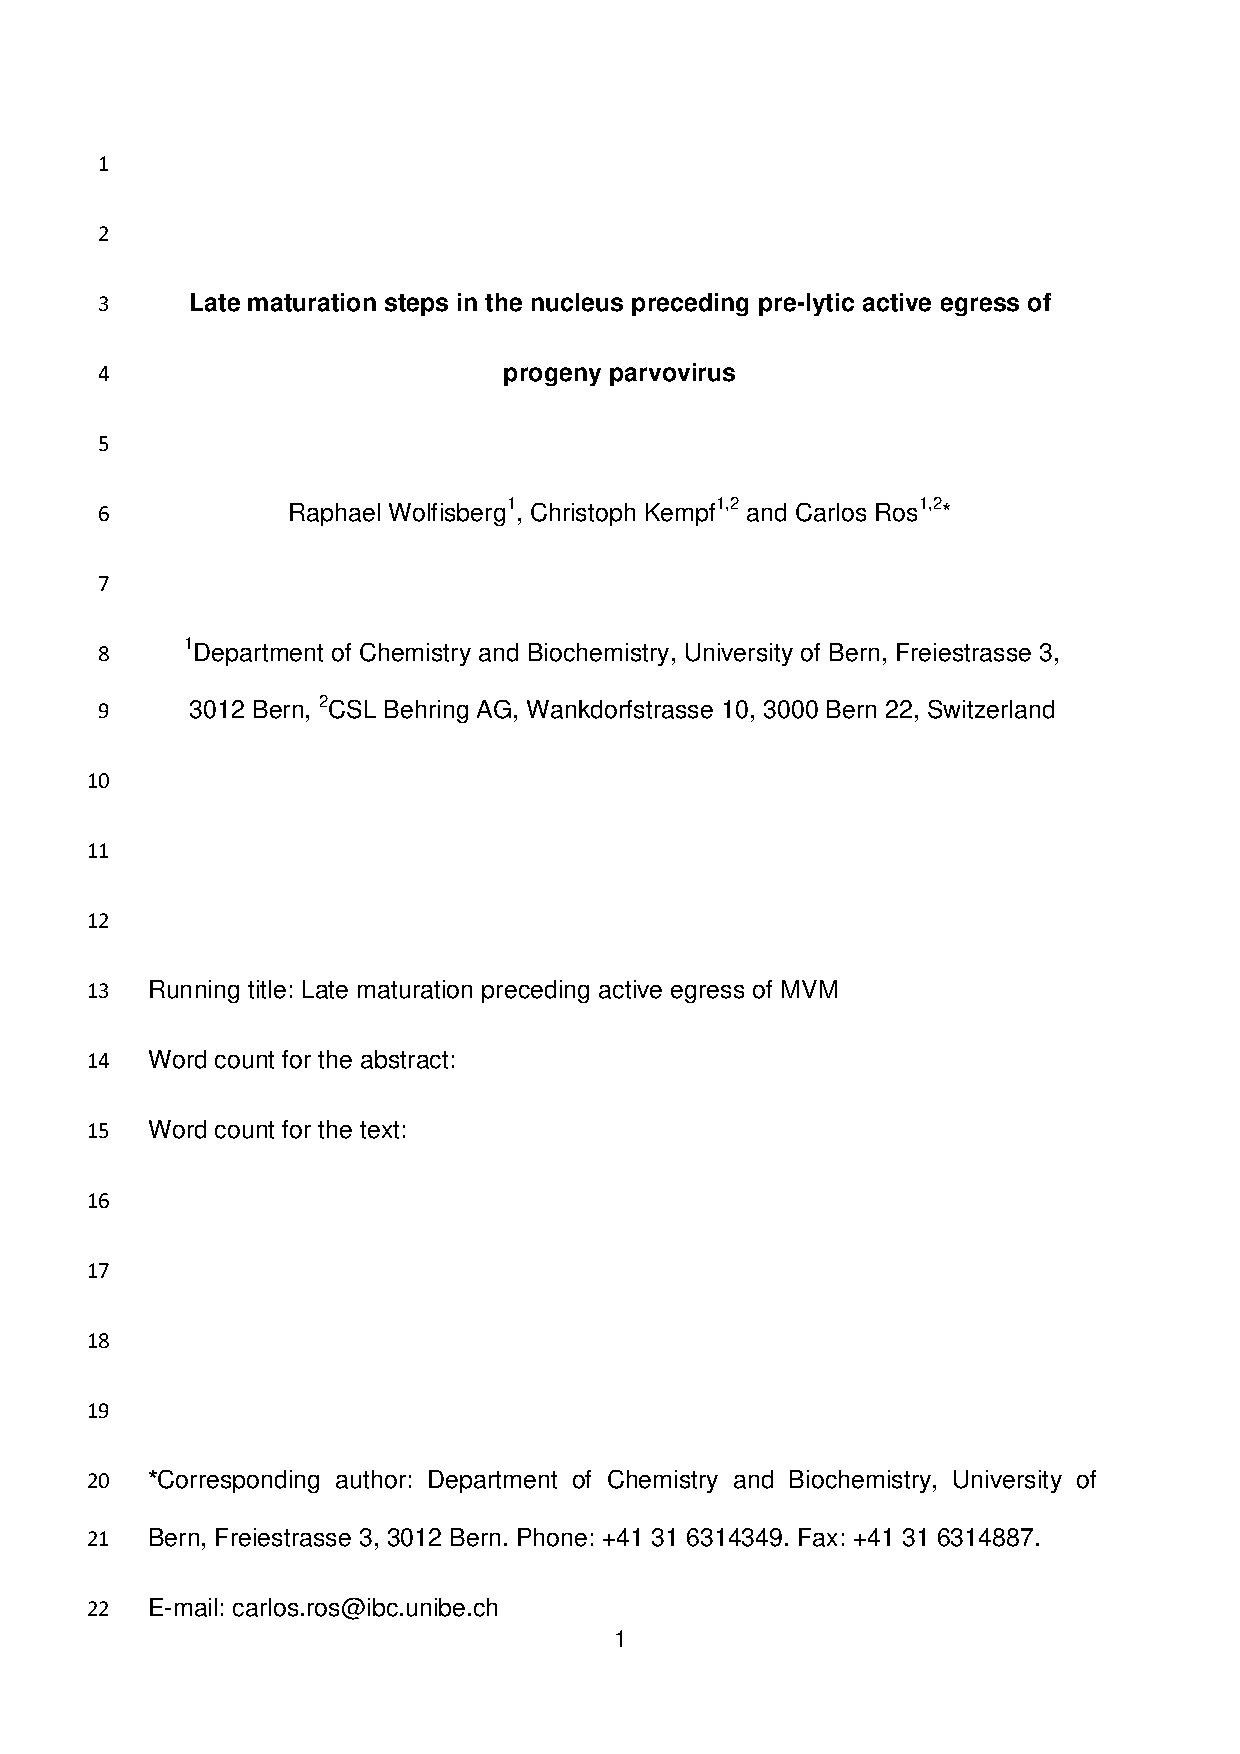
\includepdf[pagecommand=\thispagestyle{empty}, pages={1-34}, scale=1]{../pdfdocuments/TEST}
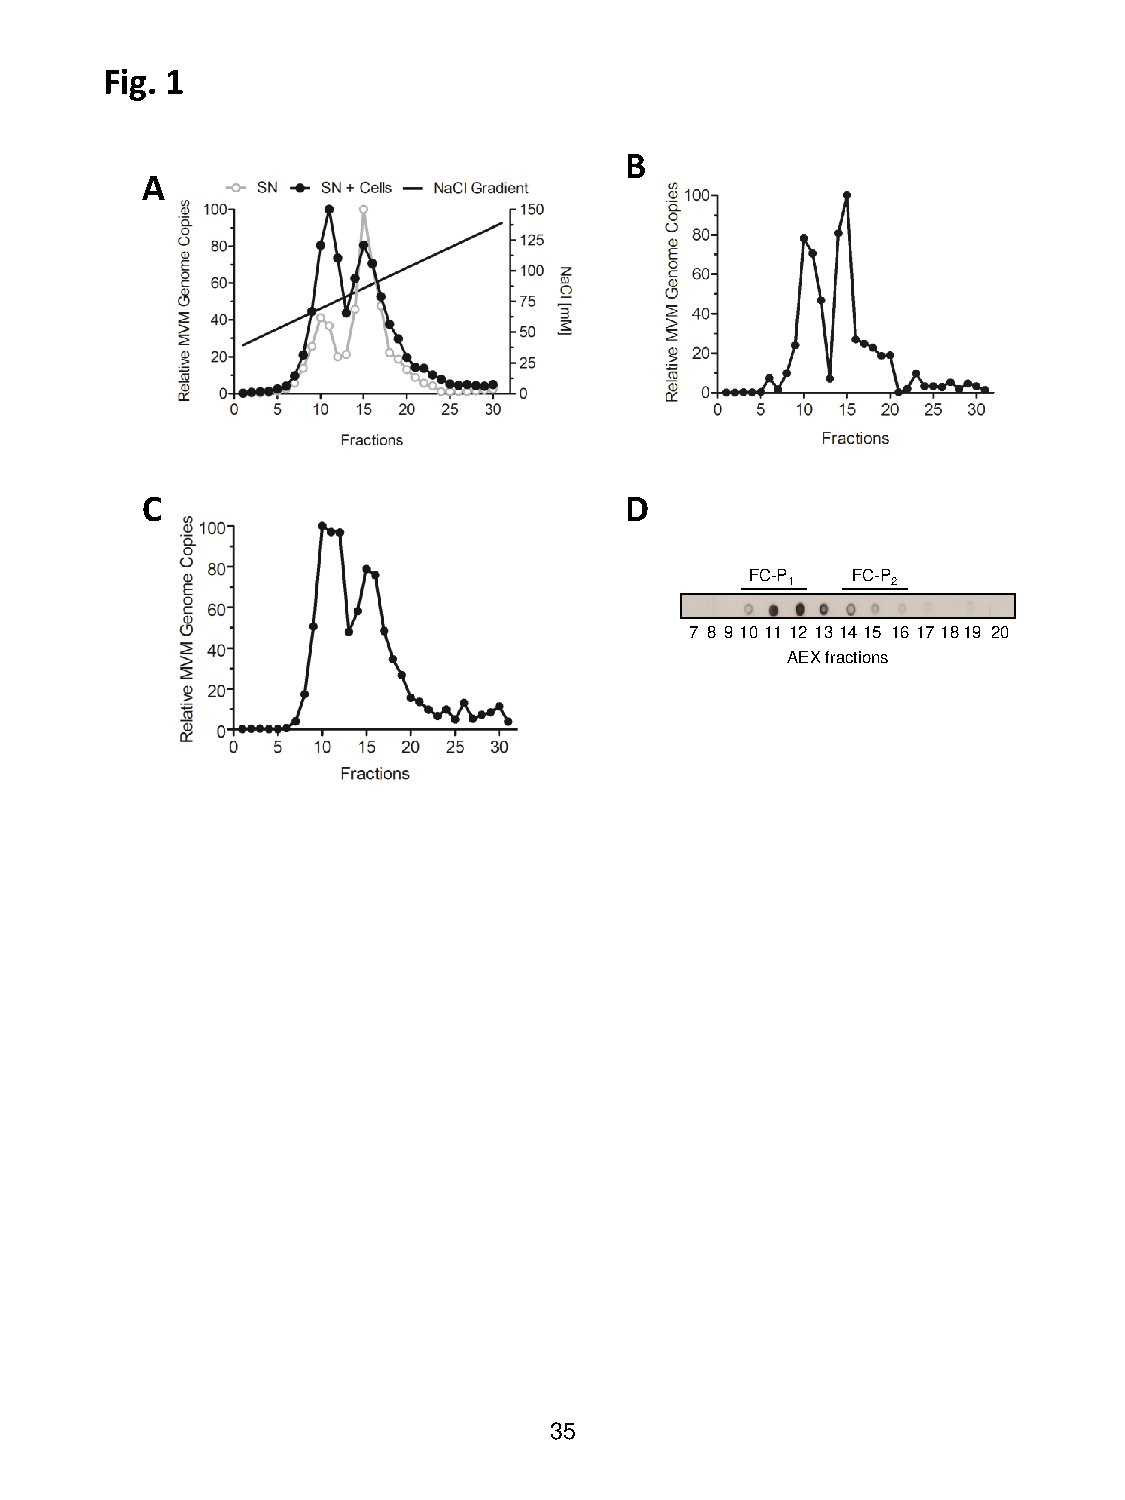
\includepdf[pagecommand=\thispagestyle{empty}, pages={1-8}, scale=1]{../pdfdocuments/FIGURES}

\label{ChapterPub1End}








\part{Discussion}


%----------------------------------------------------------------------------------------
% BIBLIOGRAPHY
%----------------------------------------------------------------------------------------

\pagestyle{raphimen}
\bibliographystyle{abbrvnat}
\begin{scriptsize}
\bibliography{MyBib}
\end{scriptsize}
%\bibliographystyle{jcp-tit}


\end{document}